% Based on the University of Calgary thesis template by
% N. Mancell (1998,2006), D. Teale (1992), and T. Zhang (2012)


% Werid fix needed to get colour working with graphicx
\makeatletter
\let\my@xfloat\@xfloat
\makeatother
\documentclass[12pt]{ucalgthes1}
\makeatletter
\def\@xfloat#1[#2]{
	\my@xfloat#1[#2]%
	\def\baselinestretch{1}%
	\@normalsize \normalsize}
\makeatother
% end of fix


\usepackage[utf8]{inputenc} % unicode input
\usepackage[canadian]{babel} % hyphenation rules
\usepackage[hidelinks]{hyperref} % urls
%\usepackage[section]{placeins} % constrain figure placement
\usepackage[letterpaper]{geometry} % margins
\geometry{
  left=1in,
  right=1in,
  top=1in,
  bottom=1in,
}


% Commands to fix math spacing
\let\originalleft\left
\let\originalright\right
\renewcommand{\left}{\mathopen{}\mathclose\bgroup\originalleft}
\renewcommand{\right}{\aftergroup\egroup\originalright}


%
% Packages
%
\usepackage{amsmath}
\usepackage{algorithmic}
\usepackage{algorithm}
\usepackage{graphicx}
\usepackage{amsfonts}
\usepackage{textcomp}
\usepackage{tabularx}
\usepackage{booktabs}
\usepackage{subcaption}
\usepackage{mathspec}
\usepackage[final]{pdfpages}

\usepackage[capitalize, nameinlink, noabbrev]{cleveref}

% Font stuff
\defaultfontfeatures{Ligatures=Common, Numbers=Uppercase}
\setallmainfonts{Cambria}
\setsansfont{Calibri}
\setmonofont{Consolas}
\setmathsfont(Digits,Latin,Greek)[Numbers={Lining,Proportional}]{Cambria}
\urlstyle{sf}

% Path for figures
\graphicspath{{./images/}}


%
%    Enter your own information in these fields
%
\title{Semiregular Degenerate Refinement for 3D Discrete Global Grid Systems}
\author{Benjamin Luke Ulmer}
\thesisyear{2020}
\thesis{thesis} % can be thesis or dissertation
\newcommand{\thesistitle}{Semiregular Refinement Applied to 3D Discrete Global Grid Systems}
\monthname{JUNE}
\dept{GRADUATE PROGRAM IN COMPUTER SCIENCE}
\degree{MASTER OF SCIENCE}
%
%    End of supplied information
%


%DIF PREAMBLE EXTENSION ADDED BY LATEXDIFF
%DIF UNDERLINE PREAMBLE %DIF PREAMBLE
\RequirePackage[normalem]{ulem} %DIF PREAMBLE
\RequirePackage{xcolor}
\providecommand{\DIFadd}[1]{{\protect\color{blue}\uwave{#1}}} %DIF PREAMBLE
\providecommand{\DIFdel}[1]{{\protect\color{red}\sout{#1}}}                      %DIF PREAMBLE
%DIF SAFE PREAMBLE %DIF PREAMBLE
\providecommand{\DIFaddbegin}{} %DIF PREAMBLE
\providecommand{\DIFaddend}{} %DIF PREAMBLE
\providecommand{\DIFdelbegin}{} %DIF PREAMBLE
\providecommand{\DIFdelend}{} %DIF PREAMBLE
%DIF FLOATSAFE PREAMBLE %DIF PREAMBLE

%DIF END PREAMBLE EXTENSION ADDED BY LATEXDIFF


\begin{document}
\makethesistitle
\pagenumbering{roman}     % resets page counter to one
\setcounter{page}{2}
%\chapter*{UNIVERSITY OF CALGARY \\ FACULTY OF GRADUATE STUDIES}
%\thispagestyle{empty}
%The undersigned certify that they have read, and recommend
%to the Faculty of Graduate Studies for acceptance, a \Thesis\ entitled
%``\thesistitle'' submitted by \Author\
%in partial fulfillment of the requirements for the degree of
%\Degree.\\

%
%    Substitute  List of Examiners
%
%\begin{signing}{Department of Academic Computing}
%\signline
%Chairman, Dr.~John D.~Doe \\
%Department of Academic Computing \\
%Services  \\
%\signline
%Chairman, Dr.~John D.~Doe \\
%Department of Academic Computing \\
%Services  \\
%\signline
%Chairman, Dr.~John D.~Doe \\
%Department of Academic Computing \\
%Services  \\
%\signline
%Chairman, Dr.~John D.~Doe \\
%Department of Academic Computing \\
%Services  \\
%\newsigncolumn         use this command to start a new column if necessary
%\newsigncolumn
%\signline
%Chairman, Dr.~John D.~Doe \\
%Department of Academic Computing \\
%Services  \\
%\signline
%Dr.~Jane Smith \\
%Department of Academic Computing  \\

%\signline
%Dr.~A.~B.~Brown \\
%Department of Academic Computing  \\
%\end{signing}
%
\newpage
\phantomsection
\altchapter{\bf{Abstract}}
Recent technological advancements have led to unprecedented amounts of 3D data becoming available about the Earth.
Hierarchical partitionings of the surface of the Earth, known as Discrete Global Grid Systems (DGGS), have proven to be useful tools for integrating data on the Earth's surface; however, they have no native support for 3D data. Instead, a 3D version of this data structure is needed. In this thesis, we explore a particular class of refinement methods, which we term semiregular degenerate, as a potential solution to reduced cell size and compactness near the central singularity seen in typical approaches for a 3D DGGS.
We propose both a modification of an existing 3D DGGS to improve its volume preservation properties and a general framework for extending any existing DGGS to the third dimension. We also derive a set of mapping functions that facilitate efficient encoding and decoding algorithms for both these methods.

\newpage
\phantomsection
\altchapter{\bf{Acknowledgements}}
Placeholder for acknowledgements.

\begin{singlespace}
\newpage
\phantomsection
\tableofcontents
\pagestyle{plain}
\newpage
\phantomsection
\listoftables
\pagestyle{plain}
\newpage
\phantomsection
\listoffigures
\pagestyle{plain}
\clearpage
\clearpage          % otherwise tables will be numbered wrong
\end{singlespace}


\pagenumbering{arabic}

\chapter{Introduction} \label{chap:introduction}
Hook paragraph; work in progress.
Main points will be:
Earth is vast;
Earth is diverse;
Earth is important (home to all of humanity/all life).
Therefore, important to understand the Earth so we can make informed decisions regarding it.

%Yet despite the cosmic insignificance of the Earth, all of humanity---and in fact all life we are aware of---call this planet home. From the [] of the [] to the [] of the [], the Earth is both vast and diverse. Given that Earth is the [], humanity has collected large amounts of data the planet.  Likewise, the data available about the Earth is similarly vast and diverse. 

%Given its significance to all of humanity, it is vital to understand and protect the Earth.

One of the ways humanity works toward better understanding the Earth is by gathering data about it.
Remote sensing satellites and aircraft, along with various smart technologies, have created a significant increase in the amount of geospatial data available and continually being collected.
These developments have led to the challenge of \textit{geospatial big data}, meaning that the volume and complexity of data exceed the capacity of current computing systems~\cite{lee2015geospatial}.
With applications in urban planning, agriculture, education, natural disaster prediction and management, and many other fields, the development of technologies for managing geospatial data is more crucial than ever.
These tools are needed to efficiently integrate, process, analyze, and visualize geospatial data in order to use it to make informed decisions.
Such a need has led to the vision of Digital Earth, where all data regarding the Earth is available in a common reference used by the public to inform their decisions.
The use of such a system would range from world governments informing policy by analyzing climate trends to homeowners referencing local utility line locations when building a fence.
In reality, such an expansive and holistic system is yet to be achieved; however, many approaches for smaller scope Digital Earths exist.


Geographic information systems (GIS) are one of the conventional approaches used for creating a Digital Earth.
With a GIS, different datasets are represented and stored as individual map layers in a planar coordinate system, which acts as a proxy for the Earth.
These individual layers are overlayed to create a complete model of the Earth (or region of the Earth) and combined with different operations to perform various analyses.
However, being created and gathered by diverse organizations, geospatial data exists in many different formats and resolutions.
The conventional GIS pipeline---which requires experts to clean, process, integrate, and distribute data---is unsustainable in the face of geospatial big data.
Furthermore, even after integrating data with a GIS, overlay operations such as intersections and data extraction are computationally expensive when many data layers are present~\cite{wang2015improving}.
Coordinate based representations of geospatial data also do not provide proper facilities to represent the uncertainty or error of the data they are used to represent~\cite{goodchild2018reimagining}.


Another challenge with GIS is the use of a flat map as the underlying representation.
Flattening the Earth produces inevitable map edges and distortion that impact the analysis and visualization of geospatial data.
Map edges can cause serious misunderstanding of the continuity between different sides of the map---especially with young children~\cite{hennerdal2015beyond}---and also affect the estimation of distance even when the continuity is correctly understood~\cite{hruby2016journey}.
Distortion causes inaccuracies in calculations such as geodesics and buffering if using planar geometry~\cite{flaterbuffering}, which is especially problematic when working with large distances and areas.
These distortions also affect the visual analysis of data by misrepresenting the size and shape of different regions.


Model globes avoid many of the shortcomings of planar maps by providing a more accurate reference model for the Earth.
Despite this, the ability for physical maps to be easily made and stored, display the entire Earth at once, and accommodate any scale has made them the preferred option in many situations.
With the advent of a Digital Earth, however, many the drawbacks of physical globes are lessened or negated.
Computer graphics algorithms and hardware allow rendering of globes in real-time, storage is no different than for a digital map, and interactive systems allow zooming and panning to show any part of the Earth at any scale.
The only challenge unsolved is displaying the entire Earth at once; however, even this is partially addressed with multi-view focus plus context rendering techniques~\cite{sherlock2017visualizations}
Because of this, there has been a recent push toward globe based Digital Earth systems, one of the most well-known examples of which being Google Earth\footnote{\url{https://www.google.com/earth/}}.
In these systems, data is visualized on a 3D model of the Earth---approximated as a sphere or ellipsoid---as opposed to a traditional planar map. While globe based Digital Earths are becoming more popular, many of these systems still use a flat map as the underlying representation for geospatial data.
Thus, these systems still suffer errors introduced by distortion resulting from any planar operations done with the underlying coordinate system.


A common approach to avoid coordinate-based representations of geospatial data is to use an area- or cell-based representation.
A partition of the Earth into a set of non-overlapping cells allows information to be associated with the cells(s) that correspond with the appropriate region(s) of the Earth.
Such partitionings are termed discrete global grids (DGG).
To accommodate different resolutions of data, a hierarchy of these DGG's at successively finer resolutions, referred to as a discrete global grid system (DGGS), is used.
Not only does this cell hierarchy allow multiple resolutions of data to be supported, but it also provides an inbuilt mechanism for representing data uncertainty by using a cell (or set of cells) to represents the range of possible locations for a datum.
However, in order for DGGS cells to serve as a suitable representation for geospatial data, these cells should be compact and near-uniform in size.
Compact cells ensure that data from geographically distant (relative to the size of the cell) locations are not represented in the same cell.
Uniformity of size ensures that each resolution of the DGGS represents the entire Earth at a particular spatial resolution and that cells of the same size do not appear at different resolutions of the grid system.


While DGGS's are an effective tool for integrating and managing geospatial data on the surface of the Earth, they have no inbuilt mechanism for supporting 3D data.
Many of today's geospatial sensors, along with other technologies such a numerical weather prediction, generate data with an associated altitude in addition to other dimensions.
With a DGGS, 3D data is flattened with altitude stored only as an attribute.
This shortcoming has motivated the development of volumetric (3D) discrete global grids and grid systems to allow native support for 3D data.
Going forward, we use the term 3D DGGS to refer to these technologies collectively.


Most human activity and interest, and correspondingly geospatial data, is located in a relatively small region above and below the surface of the Earth ($\pm$10 -- 500 km).
Likewise, most existing approaches for 3D DGGS's have focused on this region.
However, there are select processes such as seismic wave propagation and the magnetosphere that span much beyond this region.
Furthermore, the range of altitudes satellites orbit at is extensive, with satellites in high Earth orbit exceeding 36,000 km.
Therefore, to support the full range of human activity and interest, 3D DGGS's that extend to the centre of the Earth and far beyond the atmosphere are needed.


\section{Problem Statement} \label{chap:1:problem}
Despite the necessity for 3D DGGS's, the area of research is still relatively unexplored compared to that of traditional DGGS and GIS technologies.
Additionally, of the proposed methods, many are only appropriate for data with small altitude ranges, or data near the surface of the Earth.
Thus, for data with more extensive altitude ranges, there are even fewer methods that are appropriate. 
From this, we arrive at the primary goal of this thesis: to develop 3D DGGS's that have adequate support for unbounded ranges of altitude. 


A simple approach for such a 3D DGGS would be to embed the Earth in a 3D Euclidean voxel partitioning or similar space partitioning data structure, for which many efficient and well-tested algorithms exist.
While such a system is simple in its construction, it ignores the spherical nature of the Earth.
Cells are not aligned with the surface of the Earth, which means there is no consistent orientation of up (increasing altitude) and down (decreasing altitude) with respect to a cell.
Likewise, traversal along the surface of the Earth is complex and requires ``zig-zagging'' up and down.
This type of grid also provides a poor approximation for the surface of the Earth, especially at low resolutions.
While these issues are negligible for small-scale regions of the Earth, for a 3D DGGS with global coverage, the underlying grid should be sphere-based and Earth-centric.
Cells should be aligned with the surface of the Earth and have a consistent orientation for increasing and decreasing altitude.


\begin{figure}[h]
	\centering
	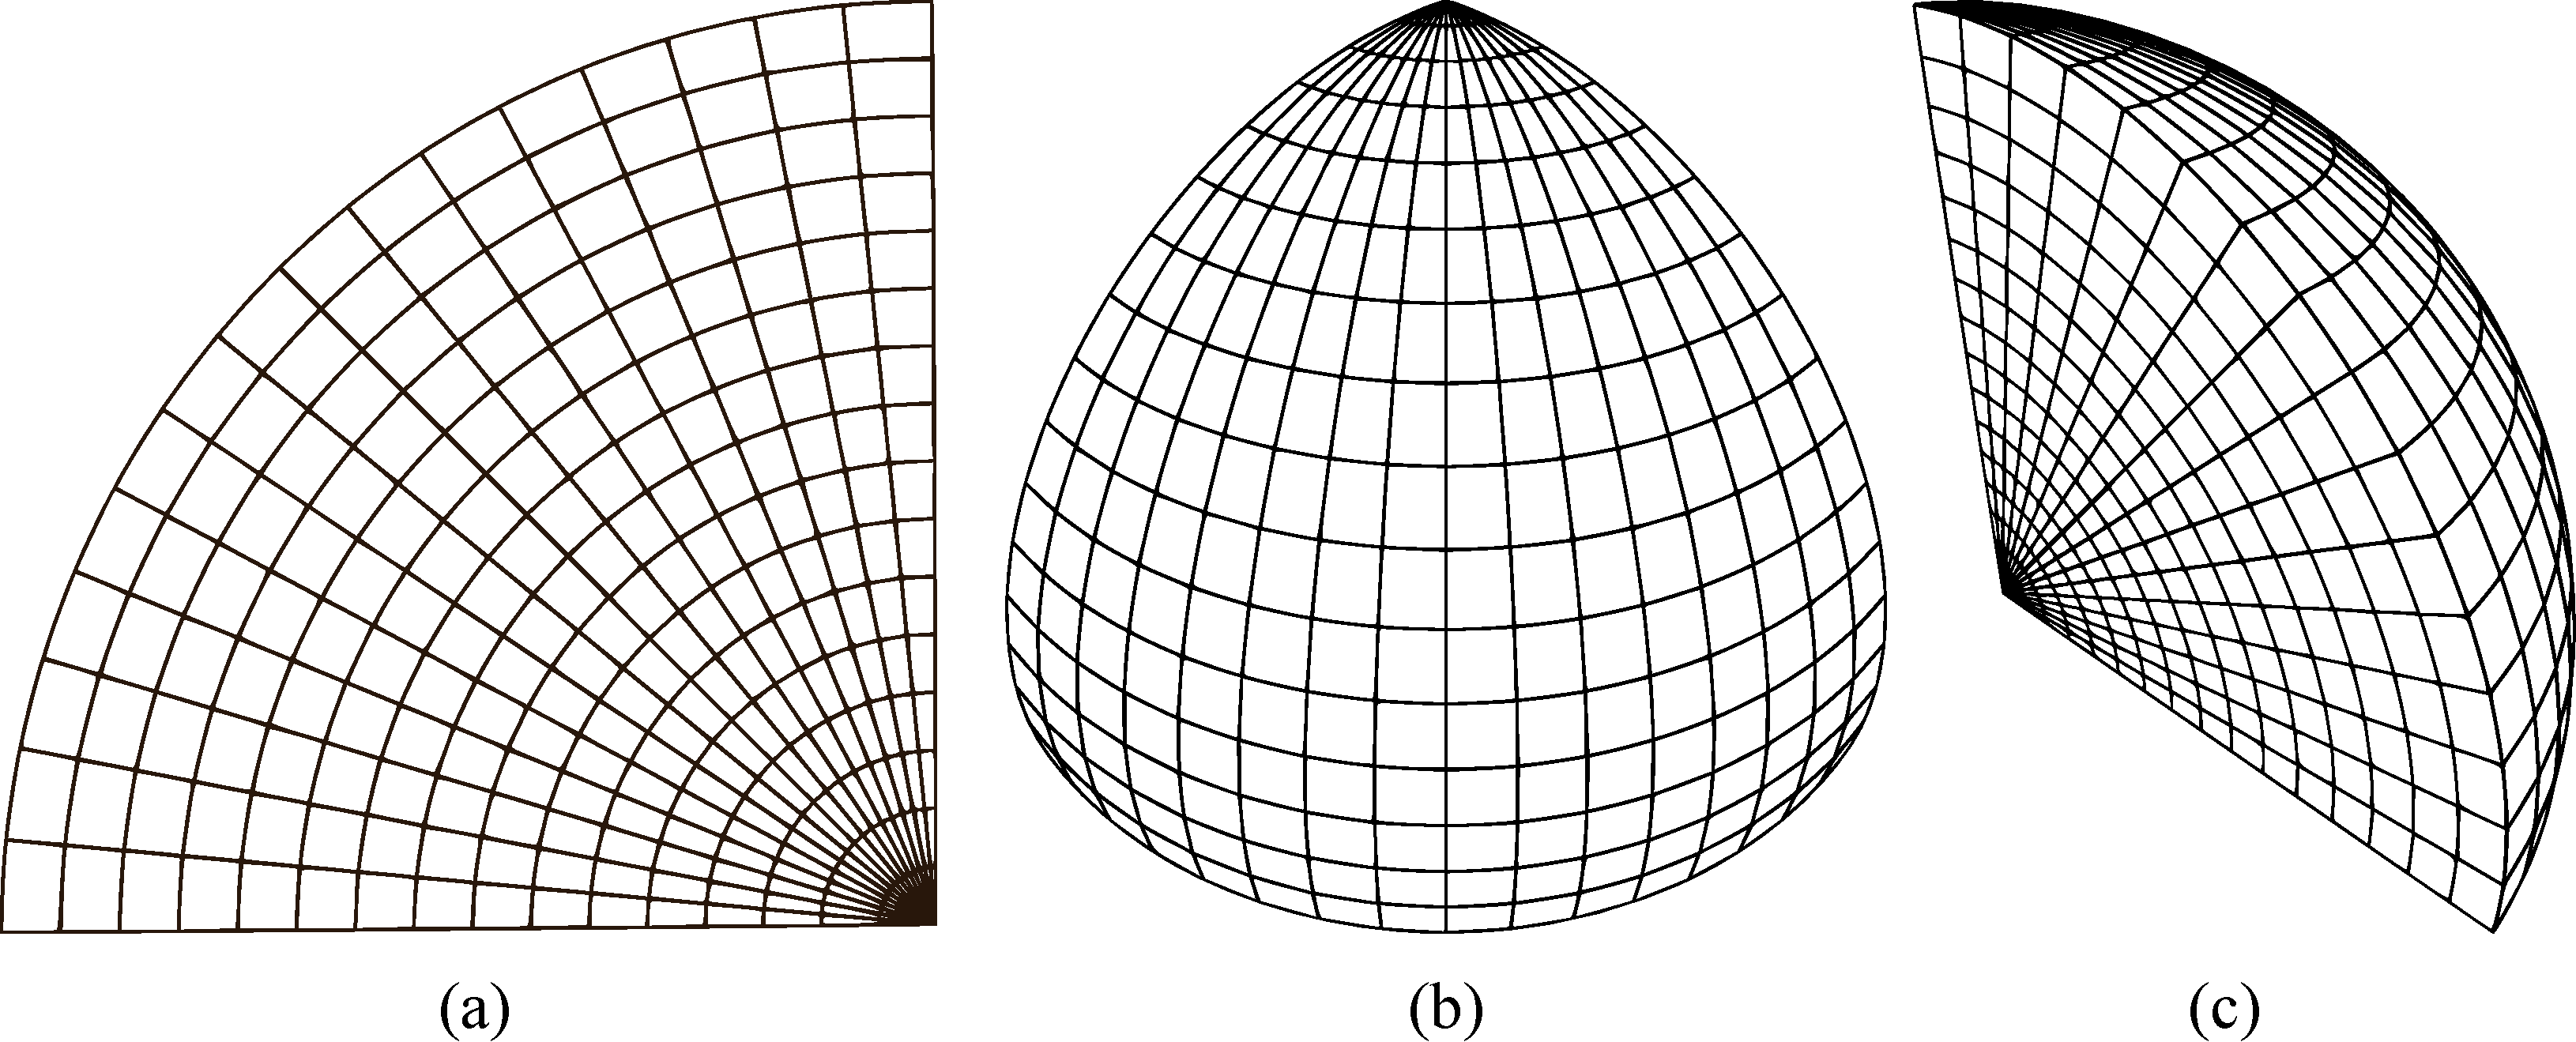
\includegraphics[width=\textwidth]{3dllg.pdf}
	\caption[Different Views of a 3D Latitude-Longitude Grid]{
		Placeholder figure.
		Caption describing degeneration in cells toward centre and poles
	}
	\label{fig:3dllg}
\end{figure}


The main challenge associated with such Earth-centric grids is the inevitable degeneration of cells toward the singularity at the centre of the Earth.
This effect is demonstrated in Figure~\ref{fig:3dllg}---cells more near the centre of the grid become increasingly small and skinny and eventually degenerate to pyramids.
For grids with a small radial extent, the effect of this is negligible; however, for the range of altitudes we wish to support in this thesis, it cannot be ignored.
The problem with this type of cell degeneration is two-fold, as it reduces both the compactness and volume of cells.
Furthermore, the resulting difference in the volumes of cells is unbounded.
It is worth noting that this same issue presents itself in traditional latitude-longitude grids at the poles, also demonstrated in Figure~\ref{fig:3dllg}.
Addressing such cell degeneration is one of the main challenges of this thesis.



\section{Goals and Scope} \label{chap:1:goals}
In addition to the initial goal of supporting an unbounded range of altitudes, there are several other aims for a 3D DGGS we wish to explore in this thesis.
While we discuss these below in the context of a 3D DGGS, they are equally applicable to their conventional 2D counterparts.
We choose to explore these goals only for Earth-centric 3D DGGS's using semiregular degenerate refinement strategies (see Chapter~\ref{chap:3:semiregDegen}); limiting the scope in this manner allows a more thorough exploration of the goals in the 3D DGGS's we propose.


As discussed previously, the cells of a 3D DGGS need to be compact while also maintaining near-uniform volume.
Ideally, all cells of the grid would be exactly congruent; however, with an Earth Centric grid, this is impossible.
Therefore, for our 3D DGGS's, we aim to have cells with similar shapes and sizes without sacrificing compactness.
In addition to near-uniform volume, cells being \textit{exactly} equal volume is beneficial in specific applications.
Calculating the volume of a cell can be an expensive operation, which significantly impacts the speed of analysis if this property is needed frequently.
If all cells have the same size, this calculation is replaced with a constant resulting in a significant performance increase in these applications.
Thus, we also aim to have perfectly equal volume cells in our 3D DGGS's when it is possible and desired to do so.


Once the cells of a 3D DGGS are defined, methods for mapping geospatial data to the appropriate set of cells are needed.
Likewise, the inverse process of mapping data associated with a set of cells back to the corresponding regions of the Earth is needed for visualizing data on the globe.
These two operations are referred to as grid encoding and grid decoding (or just encoding and decoding), respectively, and allow the integration of geospatial data with the grid system.
With data integrated, analyses such as region growing and data aggregation require spatial neighbourhood and hierarchy traversal queries.
Ensuring all these operations are efficient allows quick integration, processing, analysis, and visualization of data with the 3D DGGS.


Finally, our 3D DGGS should leverage the accomplishments already made with conventional DGGS to facilitate the efficient and straightforward transference of data between 2D and 3D DGGS's. This interoperability allows smooth migration from 2D to 3D systems while also providing backwards compatibility from 3D to 2D systems.


Given these goals and scope, we refine the goal of this thesis: develop methods for Earth-centric 3D DGGS's using semiregular degenerate refinement to support unbounded ranges of altitude, equal (or near-equal) volume cells, efficient operations, and interoperability with 2D DGGS's.


\section{Methodology} \label{chap:1:method}
In this thesis, we use two different approaches to create 3D DGGS's with the desired properties.
The first approach modifies the refinement rules of an existing 3D DGGS, the Spheroid Degenerated-Octree Grid (SDOG)~\cite{yu2009sdog}, to improve its volume-preserving properties.
With SDOG, a sphere with twice the radius of the Earth is initially divided into eight equal octants via the equatorial plane and two perpendicular meridian planes.
Cells (including the initial octants) are then refined using splitting surfaces located at the midpoint of the three spherical coordinates: latitude, longitude, and radius.
The extent of these splitting surfaces (and the number of resulting children cells) depends on the shape of the cell, which prevents excessive cell degeneration near the poles and centre of the grid.
We perform the modifications by analyzing the placement of these splitting surfaces and finding ideal new locations that result in cells of the most uniform volume possible given certain constraints.


The second approach is a general method for creating a 3D DGGS that uses a conventional polyhedron based DGGS as a starting point and specification.
First, we create the initial 3D discretization by extruding the faces of the initial polyhedron of the input DGGS into prismatoid cells.
Bases of prismatoid cells are then refined using the same refinement scheme as the input DGGS and combined with a radial refinement.
Such an approach for creating a 3D DGGS allows the research, development, and data integration achieved with conventional DGGS to readily be leveraged with the 3D one.
We take care to perform the extension in such a way that it achieves the desired properties of the 3D DGGS regardless of the 2D one used.
The extension also allows for an additional property, a target aspect ratio for cells, to be attained.


For both of these approaches, we define mappings between physical points and their corresponding locations in grid space, which we use to implement efficient encoding and decoding operations.
For the SDOG based approach, we provide constant time encoding and decoding algorithms that outperform the standard versions of these algorithms at high levels of refinement.
These new algorithms can be used both with conventional SDOG and, by using the provided mappings, the volume-preserving one.
We also provide similar algorithms for the 3D DGGS's that result from the extension method.


We evaluate the effectiveness of the first approach using two metrics of volume preservation: one for the maximum difference in volumes and one for the distribution.
We also use a third metric to evaluate the impact these modifications have on the compactness of cells.
For our proposed encoding and decoding algorithms, we compare the runtime performance with the conventional algorithms at different levels of refinement both for conventional SDOG and our modified grids.


We evaluation of the second approach through a series of use cases, each employing a different combination of input DGGS and 3D parameters to create a resulting 3D DGGS most appropriate for the application.
These use cases illustrate both the versatility and sophistication of the method, being able to quickly create many different 3D DGGS's while achieving the desirable properties outlined above.


As a part of this thesis, we have implemented several components programmatically.
For both SDOG and the grid extension method, we created basic visualization frameworks for displaying the resulting grid geometries of different refinement rules.
These tools allowed quick implementation and visual analysis of different modifications to refinement, and the outputs served as the basis for many of the figures in this thesis.
For SDOG, we also implemented a tool for calculating volume and compactness statistics for different refinement methods along with both the conventional and improved encoding and decoding algorithms.
These were used for the analysis and runtime comparison, respectively.
Finally, the entire grid extension methodology was integrated with an internal research toolset used for designing and testing different conventional DGGS's.
This expanded toolset created the different 3D DGGS's employed in the use case examples.


\section{Contribution} \label{chap:1:contribution}
This main contributions of this thesis fall into three groups:

\begin{enumerate}
	\item Modifications of SDOG refinement.
	These modifications are able to achieve perfect volume preservation between all non-degenerate cells.
	Additionally, we provide blending functions that allow a balanced trade-off between volume preservation and cell compactness.
	An analysis of volume preservation and compactness for the different modifications is also provided.
	
	\item Method for extending 2D DGGS to 3D.
	This method is fully general and supports any valid DGGS, including any refinement factor and non-congruent refinement.
	Furthermore, clearly defined parameters allow for a target aspect ratio for cells and---like the SDOG modifications---a balanced trade-off between volume preservation and cell compactness.
	We use a set of sample use cases to evaluate the method.
	
	\item Mapping functions (for modified SDOG \textit{and} extended grids).
	These mappings enable the volume preservation of the above methods while still allowing efficient encoding and decoding.
	For SDOG, we also propose new constant time encoding and decoding algorithms and benchmark their performance against the standard versions.
\end{enumerate}

The method for modified SDOG refinement, along with its mappings and analysis, has been published in the journal \textit{Geoinformatica}~\cite{ulmer2020toward}.
The efficient encoding and decoding algorithms are an unpublished extension of this work.
The grid extension method, along with its mappings and use case results, has been published in the journal \textit{ISPRS International Journal of Geo-Information} in a special issue on Global Grid Systems~\cite{ulmer2020general}.


\section{Thesis Overview} \label{chap:1:overview}
\textbf{Draft based on current outline; may change.}
The outline for the remaining chapters of this thesis is as follows:
Chapter~\ref{chap:background} covers background information on map projections, Digital Earth systems, and global grids.
Chapter~\ref{chap:3ddggs} discusses the benefits and drawbacks of different approaches for creating a 3D DGGS and also provides a detailed explanation of the semiregular degenerate refinement strategy employed throughout the thesis.
Chapter~\ref{chap:sdog} introduces SDOG and provides an analysis of the number of cells in SDOG at a given resolution.
We then provided the modified refinement rules that improve volume preservation and the analysis of said rules.
Chapter~\ref{chap:extension} covers the grid extension method for creating a 3D DGGS from a 2D one.
We start with a basic version of the method for 1-to-4 refinement factors, and then introduce extensions for other factors and targeting a specific cell aspect ratio.
Chapter~\ref{chap:mapping} derives the mapping functions used for modified SDOG and the extended grids.
Chapter~\ref{chap:coding} then details how these mappings are used for efficient encoding and decoding operations.
This chapter is also where we introduce and compare the improved encoding and decoding algorithms for SDOG.
Chapter~\ref{chap:usecases} showcases three sample use cases for the grid extensions method, as well as the 3D DGGS's used for said use cases.
Finally, Chapter~\ref{chap:conclusion} concludes with a summary, along with limitations and directions for future work.

\chapter{Background and Related Work} \label{chap:background}
Providing a complete history of map and globe making (cartography) is much beyond both the scope and ability of this thesis.
Instead, we provide a brief background to illuminate how these disciplines influenced the developments of Digital Earth systems.
We discuss the different approaches for a Digital Earth, starting with traditional GIS and then discussing techniques used for globe based systems and analysis.
We also provide background and related work on discrete global grids and grid systems, looking at different methods for constructing both 2D and 3D versions of these data structures.


\section{Traditional Maps and Globes}
Cartography, the study and practice of making maps, is a mature and diverse discipline.
While there is no agreement on what is the earliest known map, several examples dating back to the 4th millennium BCE exist.
World maps are not quite as old; however, there are surviving specimens from 9th century BCE Babylonia.


In the 3rd century BCE, the ancient Greeks established that the Earth is spherical; with this came the first globes of Earth.
Despite this discovery, maps still were---and continue to be---the primary method for representing the Earth and geospatial data~\cite{hruby20182000}.
Compared to maps, globes are more expensive to manufacture and more difficult to store, transport, and make measurements on.
Maps can also represent the entire Earth at once and easily accommodate any scale.
The benefits of a flat map do not come without their disadvantages, however.
Producing a map requires flattening the spherical Earth to a flat plane, an operation known as a map projection (or simply projection), which introduces inevitable distortions and map edges.
These issues are not present on globes, and because of this, they provide a more accurate representation of the Earth than is possible with any map.


\subsection{Map Projections}
Despite the fundamental challenges associated with map projections, the many benefits of maps over globes have motivated the use and study of these operations.
Distortions in a projection (or more generally in any mapping) are measured by their effect on angles, areas, and distances.
While eliminating all distortion is impossible, specialized projection methods exist that can remove certain types of distortion.
Commonly used conformal [] and area-preserving [] projections preserve angles and areas, respectively.
Isometric projections---which preserve distances---also remove angle and area distortion, and therefore do not exist between the sphere and the plane.
However, projections that preserve only certain distances, such as all those to a certain point, are possible. []
Alternatively, some methods aim for a balanced trade-off between the different types of distortion, as opposed to eliminating a specific class. []

Since distortion cannot be completely removed,

Map edges introduced by projection can also impact people's understanding 


Map projections introduce inevitable distortion and map edges
\cite{snyder1987map}
\cite{snyder1997flattening}


Come with inevitable distortion.
Certain projections can eliminate certain types of distortion i.e. equal area, conformal, etc.
Despite this, cannot completely remove all distortion.
Cannot perfectly preserve all distances.
\cite{mathematics paper on distortion}
\cite{planar area preserving}
\cite{planar conformal}


Map edges can also introduce issues with understanding maps.
\cite{hennerdal2015beyond}
\cite{hruby2016journey}


\subsubsection{Polyhedral Projections}
Using more planes can reduce distortion.
Method known and used since at least \textbf{date}.
Drawback of introduces additional map edges when flattened.
Benefit of can be folded back into pseudo globe.
\cite{bradley1946equal}
\cite{snyder1992equal}
\cite{van2006slice}
\cite{rocsca2011uniform}
\cite{rocsca2012area}
\cite{holhocs2014octahedral}
\cite{harrison2011optimization}


\section{Digital Earth Systems}
Many existing systems for creating Digital Earth.
Many different flavours for different tasks.
Maps, streetview, Earth, GIS, etc.
\cite{mahdavi2015survey}
\cite{alderson2020digital}


\subsection{GIS}
Digital Earth based on principles and techniques of traditional geography.
Based on 2D maps.
Use map ``layers'' to represent different data sets.
Layers can be combined and used for different analysis, visualizations, etc.
Distortion can cause errors in this analysis; must use spherical analysis sometimes to avoid this.
Most systems require some amount of user expertise to clean, integrate, process data.
\cite{antenucci1991geographic}
\cite{foresman1998history}


\subsection{Globe Based Digital Earth}
Use globe as reference model as opposed to flat map.
Two approaches:
(1) use underlying flat representation and map to globe for visualization.
Does not solve issues of distortion for analysis purposes, only visualization.
\cite{goodchild2018reimagining}


Other approach is to do analysis directly in spherical or ellipsoidal space.
More computational expensive than planar equivalents, but much more accurate.
Ellipsoidal is challenging due to issues of elliptic integrals; various well known techniques for sphere however.
Raskin paper, Troy's papers, points on sphere paper, maybe others.
\cite{raskin1994spatial}
\cite{bahrdt2017rational}
\cite{alderson2016multiresolution}
\cite{alderson2019multiscale}
\cite{alderson2018offsetting}


\section{Discrete Global Grids}
Spatial partitioning structures have long been used in computer graphics for managing spatial information.
Reasons and benefits of such.
Same techniques can be used for geospatial data.
Uses of global grids varies.
From structure for speeding up queries to foundation for entire Digital Earth system (pyxis/ggs) as alternative to GIS system.
However DGG can also be used in tandem with traditional GIS technologies.
Many different techniques exist for creating such grids (and by extension grid systems).
\cite{sahr1998discrete}
\cite{sahr2003geodesic}


\subsection{Discrete Global Grid Systems}
A discrete global grid only represents Earth at one spatial resolution.
Geospatial data comes in large range of resolutions.
This can be addressed by creating a hierarchy of DGG's.
This hierarchy is what we call a DGGS.


\subsubsection{Refinement}
Start with initial discretization and then refine.
Discretization can be any DGG.


The refinement method of a DGGS defines the process by which a set of fine cells are produced from a set of coarse cells.
This should be done in a consistent manner such that it can be applied successively to create increasingly fine discretizations of the Earth.
These refinement schemes are classified by their input cell shape(s), which are given by the initial discretization; output cell shape(s), which are usually the same as the input; and their refinement factor, which is simply the ratio between the number of coarse cells and fine cells.
For example, triangle 1-to-4 (1:4) refinement produces four triangle cells for each triangle in the set of coarse cells.
The refinement factor determines how quickly the resolution of the grid increases with each application of the refinement method.


Refinement vs. subdivision: Both terms appear in the literature.
In computer graphics, subdivision typically refers to subdivision surfaces which involve repositioning vertices.
To avoid confusion, this thesis will use the term refinement to refer to the process of creating a set of children cells from parent cells.


\subsection{Spherical Grids}
Lat-long grids.
Semiregular/igloo lat-long grids (DQG).
Small circle arc grids.
Yin-yang grid.
\cite{leopardi2006partition}
\cite{sun2008global}
\cite{song2002developing}
\cite{kageyama2004yin-yang}


\subsection{Polyhedral Grids}
Main idea is to use polyhedron as approximation for sphere.
Polyhedral projection as described earlier maps spherical domain to polyhedral one.
Avoids polar degeneracies.
Area preserving projections allow equal area cells without significantly reducing compactness.
\cite{fekete1990sphere}
\cite{dutton1996encoding}
\cite{gorski2005healpix}
\cite{holhocs2014octahedral}
\cite{mahdavi2013one} % TODO ???
\cite{mahdavi2015hexagonal} % TODO ???


\subsection{3D Grids}
Same as regular grids but with altitude dimension.
Can be made from any of the above by extrusion method.
Lat-long -> 3D LLG -> GeoSOT3D.
Yin-yang -> 3D yin-yang.
Polyhedral -> frustum/prismatoid.
\cite{yoo2019concept}
\cite{sun20153d}
\cite{yoshida2004application}
\cite{kageyama2005geodynamo}
\cite{tackley2008modelling}


Issue of radial degeneration---see Chapter 3.something
Methods have been proposed that use method similar to igloo in radial dimension.
DQG -> SDOG.
SSS 3DG.
\cite{yu2009sdog}
\cite{yu2012large-scale}
\cite{yu2012lithosphere}
\cite{gang2013sphere} 
\cite{wang2013global}


\subsection{Grid Encoding and Decoding}
Need to map data/features to grid cells.
Most simple encoding is for points: find cell that contains point.
Inverse also needed: take cell and get geometry on reference model.
Call these encoding and decoding.
As part of this, need way to refer to cells uniquely.
\cite{du2018duality}


\subsubsection{Indexing Scheme} \label{sec::dggs:indexing}
For grid and cell geometries to be useful as a DGGS, a mechanism for assigning a unique index to each cell is needed.
Earth data is assigned to cells using these indices, which allows for efficient retrieval of all data associated with a specific cell or region of the Earth.
Thus, in order to be able to insert new data into the grid efficiently, it is important to be able to quickly determine the cell (and associated index) that contains a point on the Earth after it has been projected.
Likewise, given a cell index, it is important to be able to determine the geometry of the corresponding cell in the grid.
This geometry can then be inverse projected to find the region of the Earth associated with the cell.
These indices also allow for certain spatial relationship queries to be defined, such as the retrieval of neighbouring cells, and can be used to navigate up and down the hierarchy of the grid via parent and child relationships between cells in different resolutions.
\cite{yu2009coding}
\cite{vince2006indexing}
\cite{tong2013efficient}
\cite{mahdavi2015categorization}


\section{Summary}
Maps and globes have been around for thousands of years.
With advent of computer, GIS was born which carried over conventions of traditional cartography.
Recently, global grids have become popular as a replacement/augmentation of GIS.
Many different approached for DGG and DGGS.
3D DGGS are the next step of this evolution; techniques exist but still underdeveloped comparatively.

\chapter{3D Discrete Global Grid Systems} \label{chap:3ddggs}
In the previous chapter, we reviewed the DGGS as a tool for integrating multiple geospatial datasets at varying resolutions.
However, a conventional DGGS has no inbuilt mechanism for handling the altitude(s) of geospatial data.
Instead, an extension of the data structure to the third dimension---the 3D DGGS---is needed to accommodate such 3D data natively.
This chapter argues for the need for 3D DGGS's in certain applications by exploring the downsides of a typical data flattening approach used to integrate 3D data with a 2D DGGS.
We then compare the two most common approaches used for creating a 3D DGGS: embedding and Earth-centric.
We argue for the Earth-centric approach, proposing semiregular degenerate refinement---the primary tool used in the remainder of this thesis---as a strategy to lessen the disadvantages of this type of grid.


\section{Data Flattening} \label{chap:3:flatten}
A DGGS provides a multiresolution partitioning of the Earth's surface, but no partitioning in the radial dimension.
Therefore, any geospatial data with associate altitude must be flattened to the surface for integration with a DGGS, with the original altitude stored as an attribute of the data.
In applications where data \textit{does not} need to be filtered by altitude, and altitude is used no differently than any other attribute, this is an acceptable approach.
However, if data \textit{does} need to be accessed or otherwise distinguished by altitude, then this approach is problematic.
In this case, all data of a cell must be queried and searched to find those with the required altitude(s).
Furthermore, the lack of a hierarchy in the radial dimension means data at different radial resolutions must be integrated manually as opposed to using the structure of the DGGS itself to aid in this task.
Generally speaking, any benefits gained by using a DGGS are lost in the radial dimension; this is problematic for any application that uses the radial dimension as frequently as surface ones.
For example, with aircraft collision detection and avoidance, the altitude of aircraft is just as important as their geographic coordinates.
Instead of managing altitude separately, we need an extension of the 2D DGGS that hierarchically partitions altitude in addition to the surface of the Earth.
We call this a 3D DGGS.


\section{Embedded Grids} \label{chap:3:embedded}
Treating the Earth as a fully 3D entity, it seems natural to use a conventional Euclidean space partitioning data structure such as a voxel grid or octree to manage geospatial data.
We refer to this approach as an embedding one, creating an embedded 3D DGGS.
While an embedding approach is straightforward and leverages existing data structures and algorithms, it disregards the actual shape of the Earth.
Regardless of how finely refined cells are, they can only approximate the underlying representation of the Earth: a sphere or ellipsoid (\cref{fig:embedded}).
Furthermore, cells do not align with the Earth's surface, which means cells have no consistent orientation of what direction represents an increasing or decreasing altitude (up and down).
Because of this, traversing along the surface of the Earth---or any other constant altitude---becomes a non-straightforward operation that requires a ``zig-zagging'' path.
This property makes integrating geospatial data on the Earth's surface, which represents a significant portion of the data used in most applications, significantly more complicated.
It also introduces additional error, as the cells representing the data all have slightly different altitudes compared to the constant altitude of the data itself.


\begin{figure}[ht!]
	\centering
	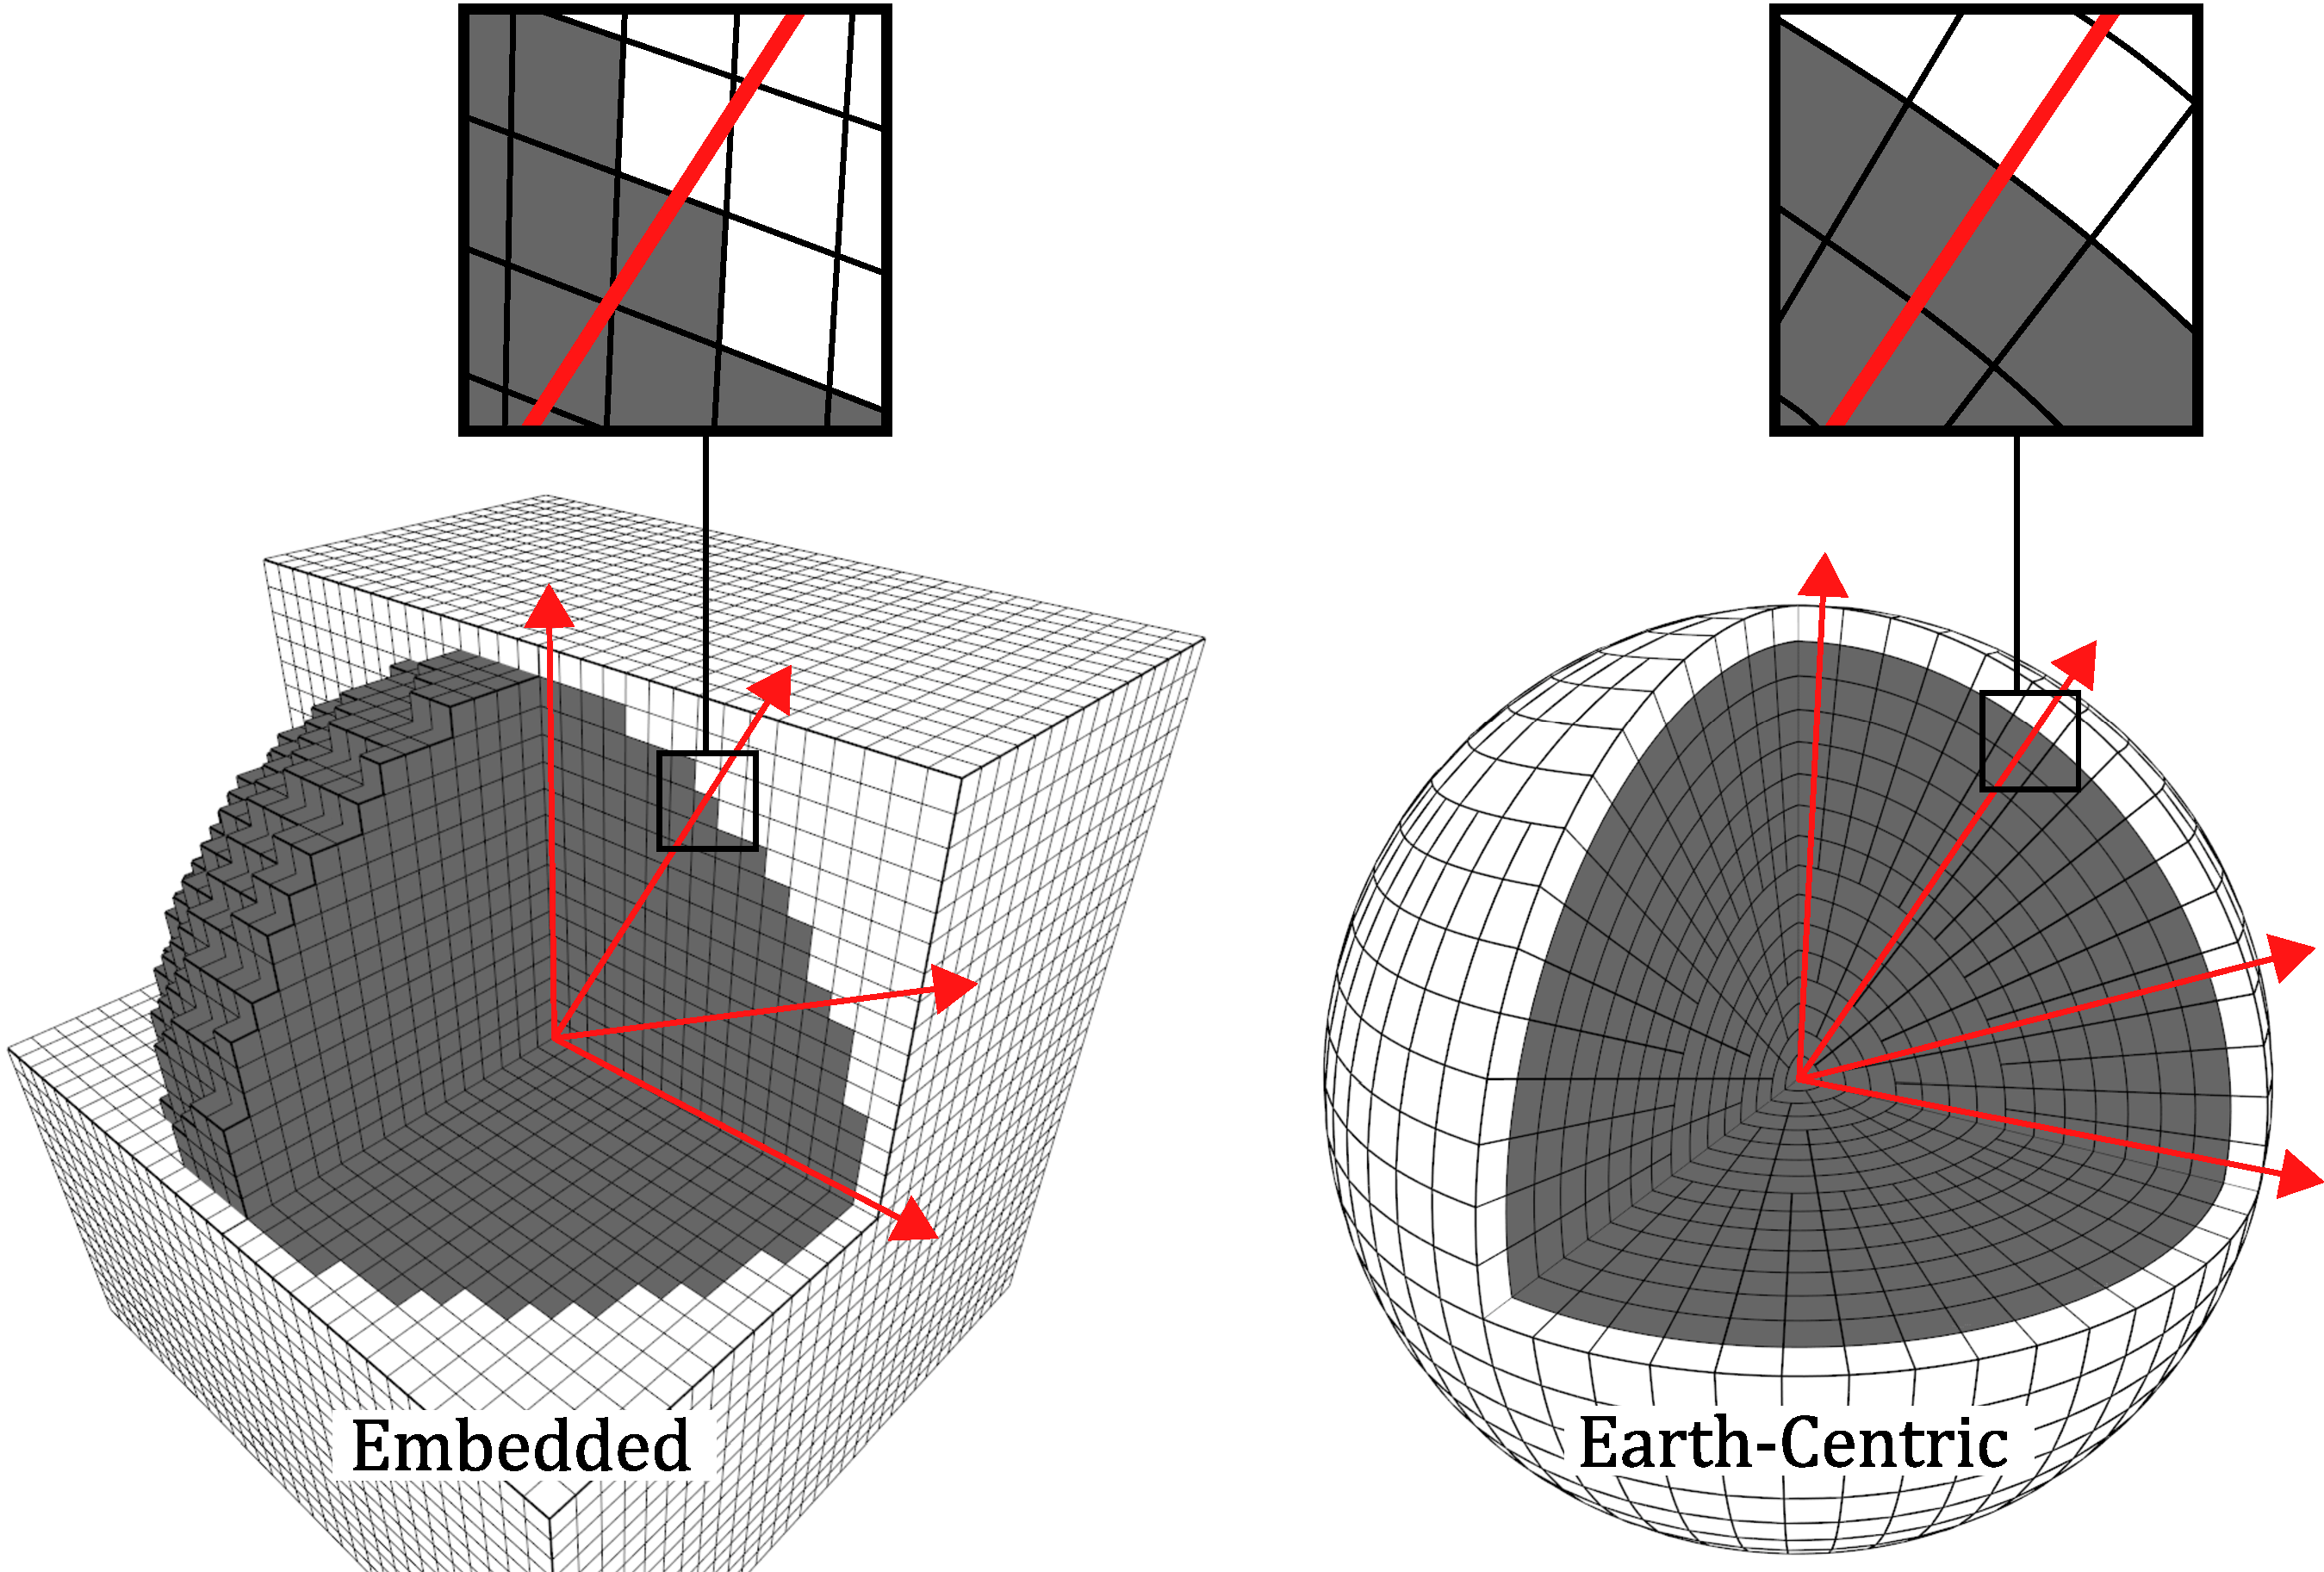
\includegraphics[width=0.85\textwidth]{embed-vs-ec.pdf}
	\caption[Comparison of embedded and Earth-centric approaches for a 3D DGGS]{
		Comparison of a (left) embedded and (right) Earth-centric 3D DGGS.
		Red arrows show directions of increasing altitude.
		Note how with the Earth-centric grid, these arrows are always orthogonal to the upper and lower boundaries of cells.
		This property does not hold in the embedded grid, with arrows intersecting the boundaries of cells at different angles depending on where the cell is located in the grid.
		Image adapted from~\cite{yu2012large-scale}
	}
	\label{fig:embedded}
\end{figure}


Despite the issues present with an embedded grid, for small-scale regions with negligible curvature, these issues also become negligible.
Because of this, embedded grids are frequently used for small-scale objects and phenomena in use cases such as surface building, rock engineering, and reservoir modelling. [citations]
However, the challenges presented by an embedding approach outweigh their benefits in the context of a 3D DGGS, which needs to have global coverage.


The inherent issues with an embedded 3D DGGS stem from the fact that their cells do not align with the Earth's surface and other layers.
Thus far, we have described 3D geospatial data as data with an associated altitude in addition to its surface coordinates, which is a spherical representation of its location.
Therefore, due to the mostly spherical shape of Earth, a 3D DGGS aligned with a sphere (or more accurately, an oblate spheroid) will also be closely aligned with the Earth.
We call this type of 3D DGGS Earth-centric.


\section{Earth-Centric Grids} \label{chap:3:earthCentric}
The most fundamental Earth-centric 3D grid is a direct extension of an LLG to the third dimension (refer back to \cref{fig:3dllg}).
In addition to diving space by latitude and longitude, a 3D LLG also divides space by equal steps in the radial dimension.
Due to the simplicity of its construction, this type of grid has seen use in global crust modelling~\cite{bassin2000current} and exploring P-wave velocity~\cite{zhao2004global}, among other applications.
The GeoSOT3D grid, proposed by Sun and Cheng, is a variation of the standard 3D LLG where latitude and longitude have been extended to larger virtual spaces to improve the efficiency of grid coding~\cite{sun20153d} and has been used to increase the efficiency of aircraft and UAV collision detection~\cite{miao2019low, zhai2019collision}.


Similar radial extensions are also possible for many of the DGG's and DGGS's explored in \cref{chap:2:DGG}.
Being composed of two component LLG's, an extension of the Yin-Yang grid to 3D can be done in the same manner as above.
These 3D Yin-Yang grids have been used extensively for geodynamo and mantle convection simulation~\cite{yoshida2004application, kageyama2005geodynamo, tackley2008modelling}.
Extensions of polyhedron-based DGGS's to 3D have also been done.
An approach by Xie et al. stacks duplicates of a DGGS at increasing radii to create a 3D global grid for interactive volumetric ray tracing of 3D Earth data~\cite{xie2013interactive}.
While this approach is appropriate for the intended use, it is not technically a 3D DGGS, as the radial component of the grid is separate from the cell hierarchy.
In order to incorporate the radial component of the grid with the cell hierarchy, Sirdeshmukh et al. create a 3D (or 4D) DGGS by placing 3D (or 4D) hypercubes on the faces of the DGGS polyhedron~\cite{sirdeshmukh2019utilizing}.
These hypercubes are then refined and traversed with a space-filling curve to create the 3D (or 4D) DGGS, which the authors use to encode point cloud data.


While using a radial extension to create a 3D DGGS is simple and effective, it results in a singularity at the centre of the Earth.
This central singularity causes the same issues near the centre of the grid as seen near the poles of an LLG---namely reduced compactness, a high valence vertex, and an unbounded difference in cell \textit{volume}.
None of the above methods address this central singularity, as these issues are mostly negligible for applications with small ranges of altitudes.
However, in accommodating large altitude ranges (as is the goal of this thesis), these issues become significant and should be addressed.


Similar to how the DQG (\cref{chap:2:spherical}) addresses polar singularities in an LLG, a similar approach can be used for the central singularity in a 3D grid.
A direct extension of the DQG to 3D, known as the spheroid-degenerated octree grid (SDOG), was proposed by Yu and Wu~\cite{yu2009sdog}.
Just as the DQG utilizes a modified quadtree refinement, SDOG extends this refinement to 3D, creating a modified octree refinement.
The resulting cells are relatively uniform in both size and shape, having a bounded maximum difference in volume.
Because of these properties, SDOG has been used for the modelling of large-scale geospatial objects~\cite{yu2012large-scale} and multi-scale visualization of the lithosphere~\cite{yu2012lithosphere}.
We provide a more detailed explanation of SDOG and its specific refinement method in \cref{chap:sdog}.
Another approach similar to SDOG is the Sphere Shell Space 3D Grid, which uses a similarly modified octree refinement of cells but is constructed from multiple spherical shells as opposed to a single sphere~\cite{gang2013sphere}.
Likewise, Wang et al. also apply a similar process to a great circle arc quaternary triangular mesh (QTM) to create a 3D DGGS~\cite{wang2013global}.
These methods all use a similar refinement strategy to handle cell degeneration toward the centre of the grid; however, the terminology used to describe this type of refinement is inconsistent between works.
In this thesis, we propose the term \textit{semiregular degenerate refinement} to describe this class of methods.

\section{3D DGGS Refinement Strategies} \label{chap:3:refinement}

\subsection{Regular Refinement} \label{chap:3:regular}

\subsection{Semiregular Degenerate Refinement} \label{chap:3:semiregDegen}
A regular grid refinement is one that results in regular connectivity in the output domain, henceforth referred to as a regular grid.
For triangular grids, this means each vertex has a valence of exactly six; for quadrilateral grids, a valence of four; and for hexagonal grids, a valence of three.


\begin{figure}[ht!]
	\centering
	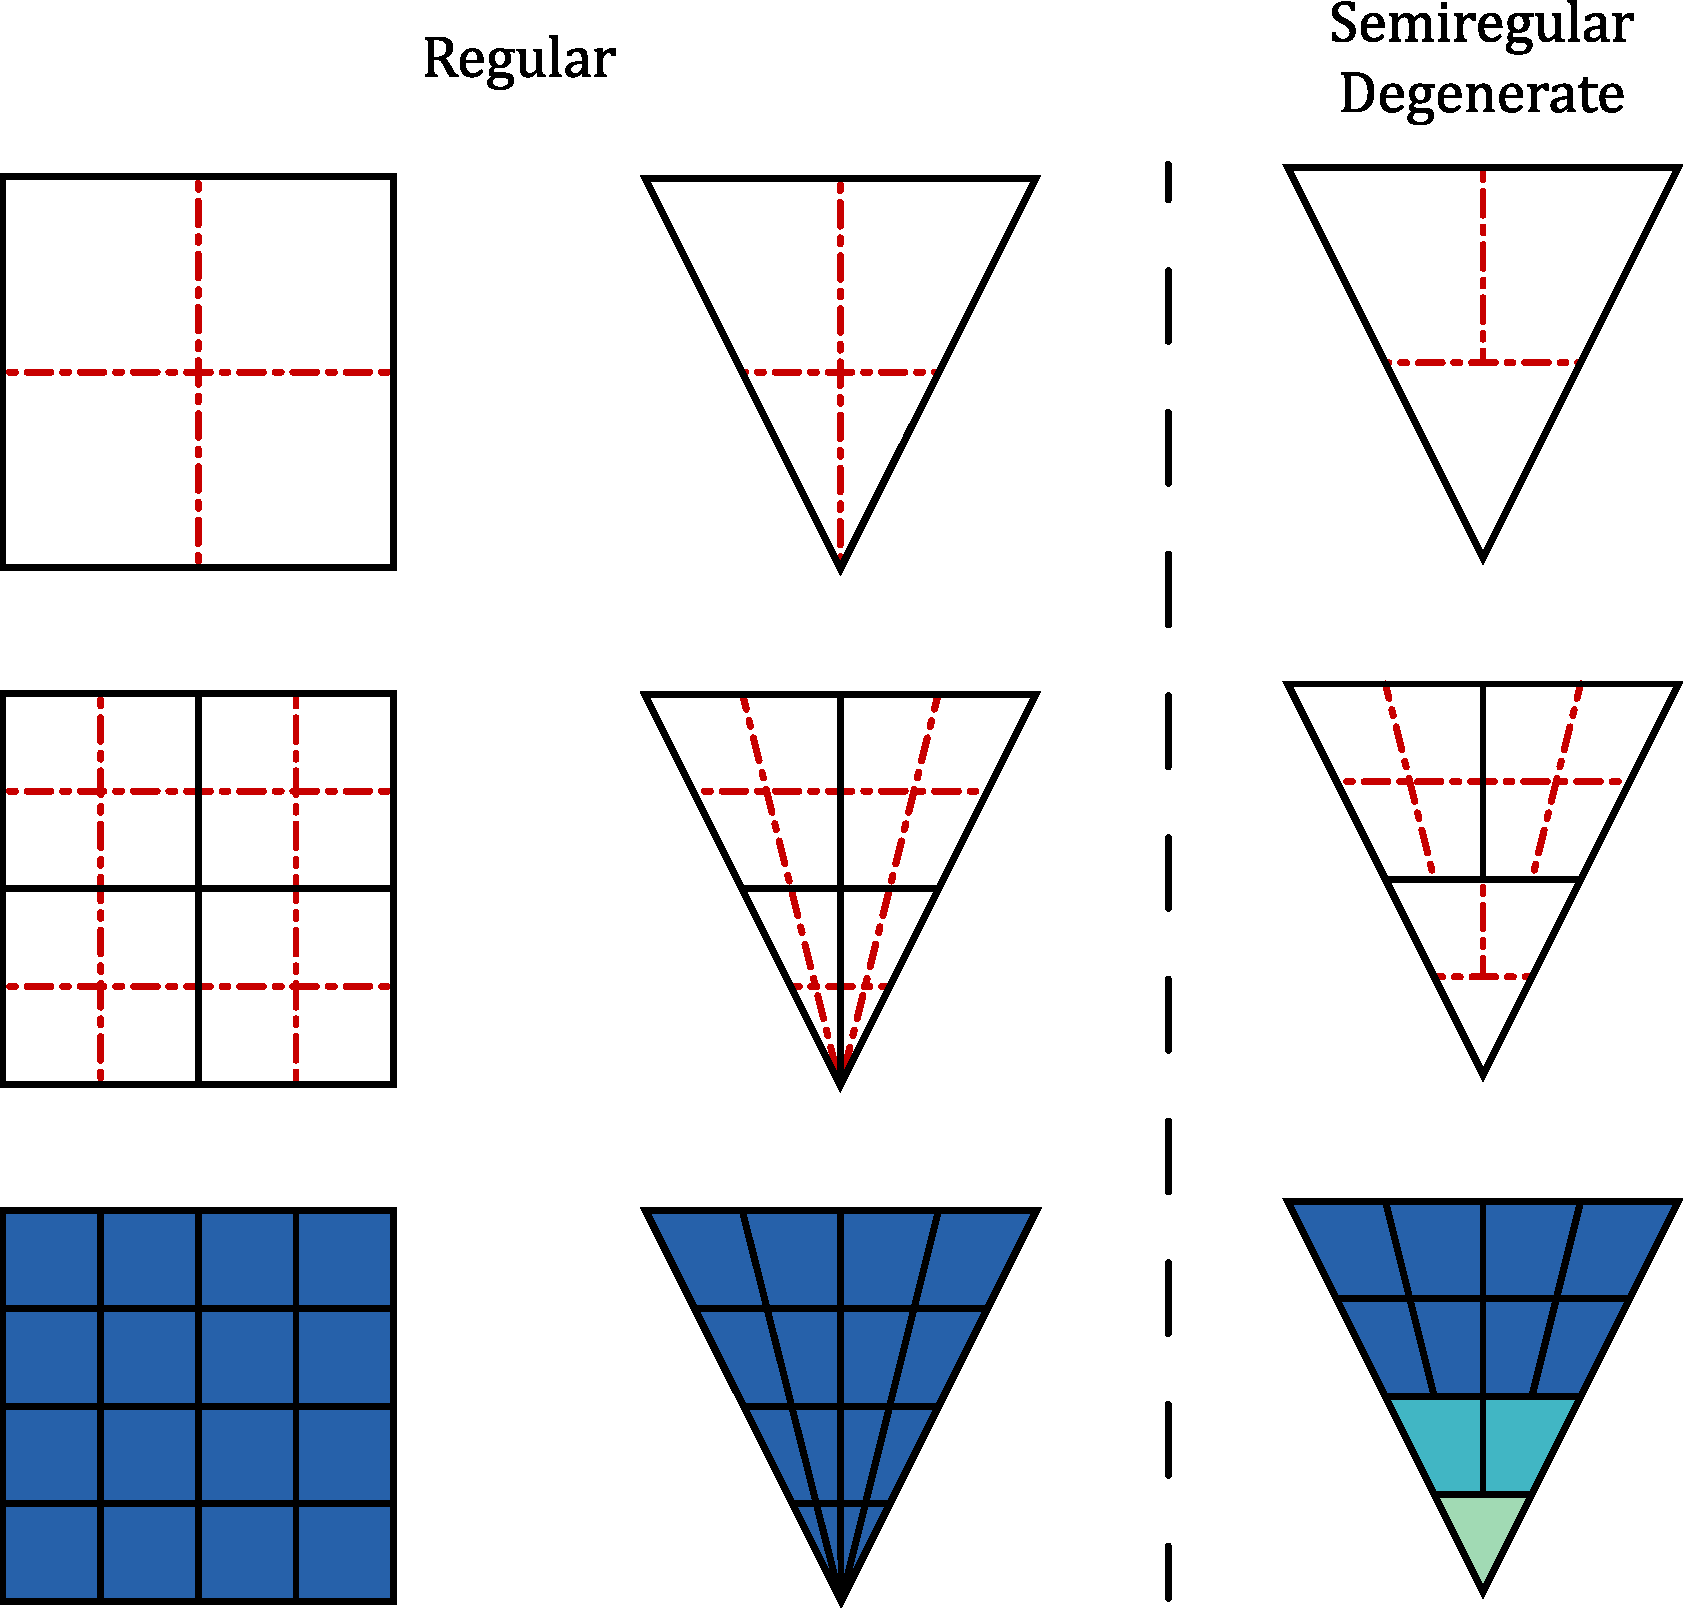
\includegraphics[width=0.7\textwidth]{semireg-degen.pdf}
	\caption[Comparison of regular and semiregular degenerate refinement]{
		A demonstration of regular and semiregular degenerate refinement schemes for quadrilaterals.
		Left: regular refinement applied to a quadrilateral domain.
		Centre: regular refinement applied to a triangular domain.
		Right: semiregular degenerate refinement applied to a triangular domain.
		The bottom row shows regions of regular connectivity in the resulting grids; note how the semiregular degenerate scheme results in several regular regions, but the grid itself is not fully regular
	}
	\label{fig:semireg-degen}
\end{figure}


Looking specifically at regular quadrilateral refinement, one way to achieve this is by splitting each input cell into four output ones with two intersecting straight lines, as shown in \cref{fig:semireg-degen}~left.
As we have seen, applying such a regular refinement to a degenerate (triangular) starting cell---such as spherical octant or a slice going from the surface of a sphere to the centre---still results in a regular grid, but the compactness and size of cells are affected (\cref{fig:semireg-degen}~centre).
To lessen this effect, the splitting edge that would normally intersect the singularity can be stopped at the other edge, as demonstrated in \cref{fig:semireg-degen}~right.
When applying this scheme recursively, only the degenerate (triangular) cells use the special refinement, and non-degenerate (quadrilateral) cells use regular refinement.
As illustrated in \cref{fig:semireg-degen}~bottom, this refinement method results in a grid with regular regions, but the grid as a whole is not itself regular.
Hence, we call this semiregular degenerate refinement.
The same principles apply in 3D for hexahedral grids; however, there are instead three intersecting \textit{faces} used in refinement.
In general, we define a semiregular degenerate refinement to be one in which one or more splitting geometries (curves in 2D and surfaces in 3D) are stopped by another splitting geometry in the direction toward a singularity where, if not stopped, would otherwise intersect said singularity.
Such a definition describes the methods used in DQG, SDOG, Sphere Shell Space 3D Grid, the great circle arc QTM extension, and those used in \cref{chap:extension} of this thesis.


A semiregular degenerate refinement allows for more uniformly sized and compact cells as compared to a regular refinement applied to the same domain.
The main drawback of this class of refinement is the degenerate connectivity introduced between the different semiregular regions of the grid.
In a non-degenerate grid, each cell will have precisely one neighbour along each edge, or no neighbours if the cell is on a boundary of the grid.
In 3D, the same applies but with faces instead of edges.
Grids resulting from semiregular degenerate refinement violate this property, with some cells having multiple neighbours along an edge/face.
Such degenerate connectivity introduces challenges when propagating values across boundaries of cells and calculating values at vertices, as is needed for finite element methods.
There has been work to address this challenge for conventional octrees~\cite{braun2008douar}, which have a similar issue between regions of the grid at different levels of refinement; similar methods could likely be applied to semiregular degenerate grids as well.
Considering the tradeoffs of this approach, we believe the benefits outweigh the disadvantages in the context of a 3D DGGS.
As such, semiregular degenerate refinement is the primary tool used in the remainder of this thesis to achieve the goals set out in \cref{chap:1:goals}.

\chapter{Volume-Preserving SDOG Refinement} \label{chap:sdog}
One of the goals of this thesis is to produce 3D DGGS's with cells of as equal volume as possible.
The first approach we use for accomplishing this is modifying an existing 3D DGGS in order to improve its volume-preserving properties.
To this end, we chose to modify SDOG, as its use of a semiregular degenerate refinement means it already satisfies the primary goal of the thesis---that is, support for unbounded ranges of altitude.
The use of spherical coordinates also allows for efficient encoding and decoding operations, which we discuss in Chapter~\ref{chap:coding}.

The content of this chapter is taken from the article "Toward Volume Preserving Spheroid-Degenerated Octree Grid," authored by Benjamin Ulmer and Faramarz Samavati, which appeared in the journal \textit{Geoinformatica}~\cite{ulmer2020toward}.
Slight modifications have been made to maintain consistent terminology with the rest of the thesis, along with a more streamlined presentation of the methodology. Furthermore, the blending method presented in this chapter is different from the one that appears in the article.


\section{SDOG Overview} \label{chap:4:sdog}
Before describing our modifications, we first provide a brief explanation of SDOG construction and refinement as initially proposed by Yu and Wu~\cite{yu2009sdog}.
SDOG is an extension of the traditional octree to a spherical, as opposed to Euclidean, volume.
A sphere with twice the radius of the Earth is initially divided into eight equal octants via the equatorial plane and two perpendicular meridian planes.
These octants are taken to be the coarsest cells of the grid and are then refined to create more fine discretizations of the sphere.
Figure~\ref{fig:sdog} shows an SDOG octant after four applications of refinement.


\begin{figure}[ht!]
	\centering
	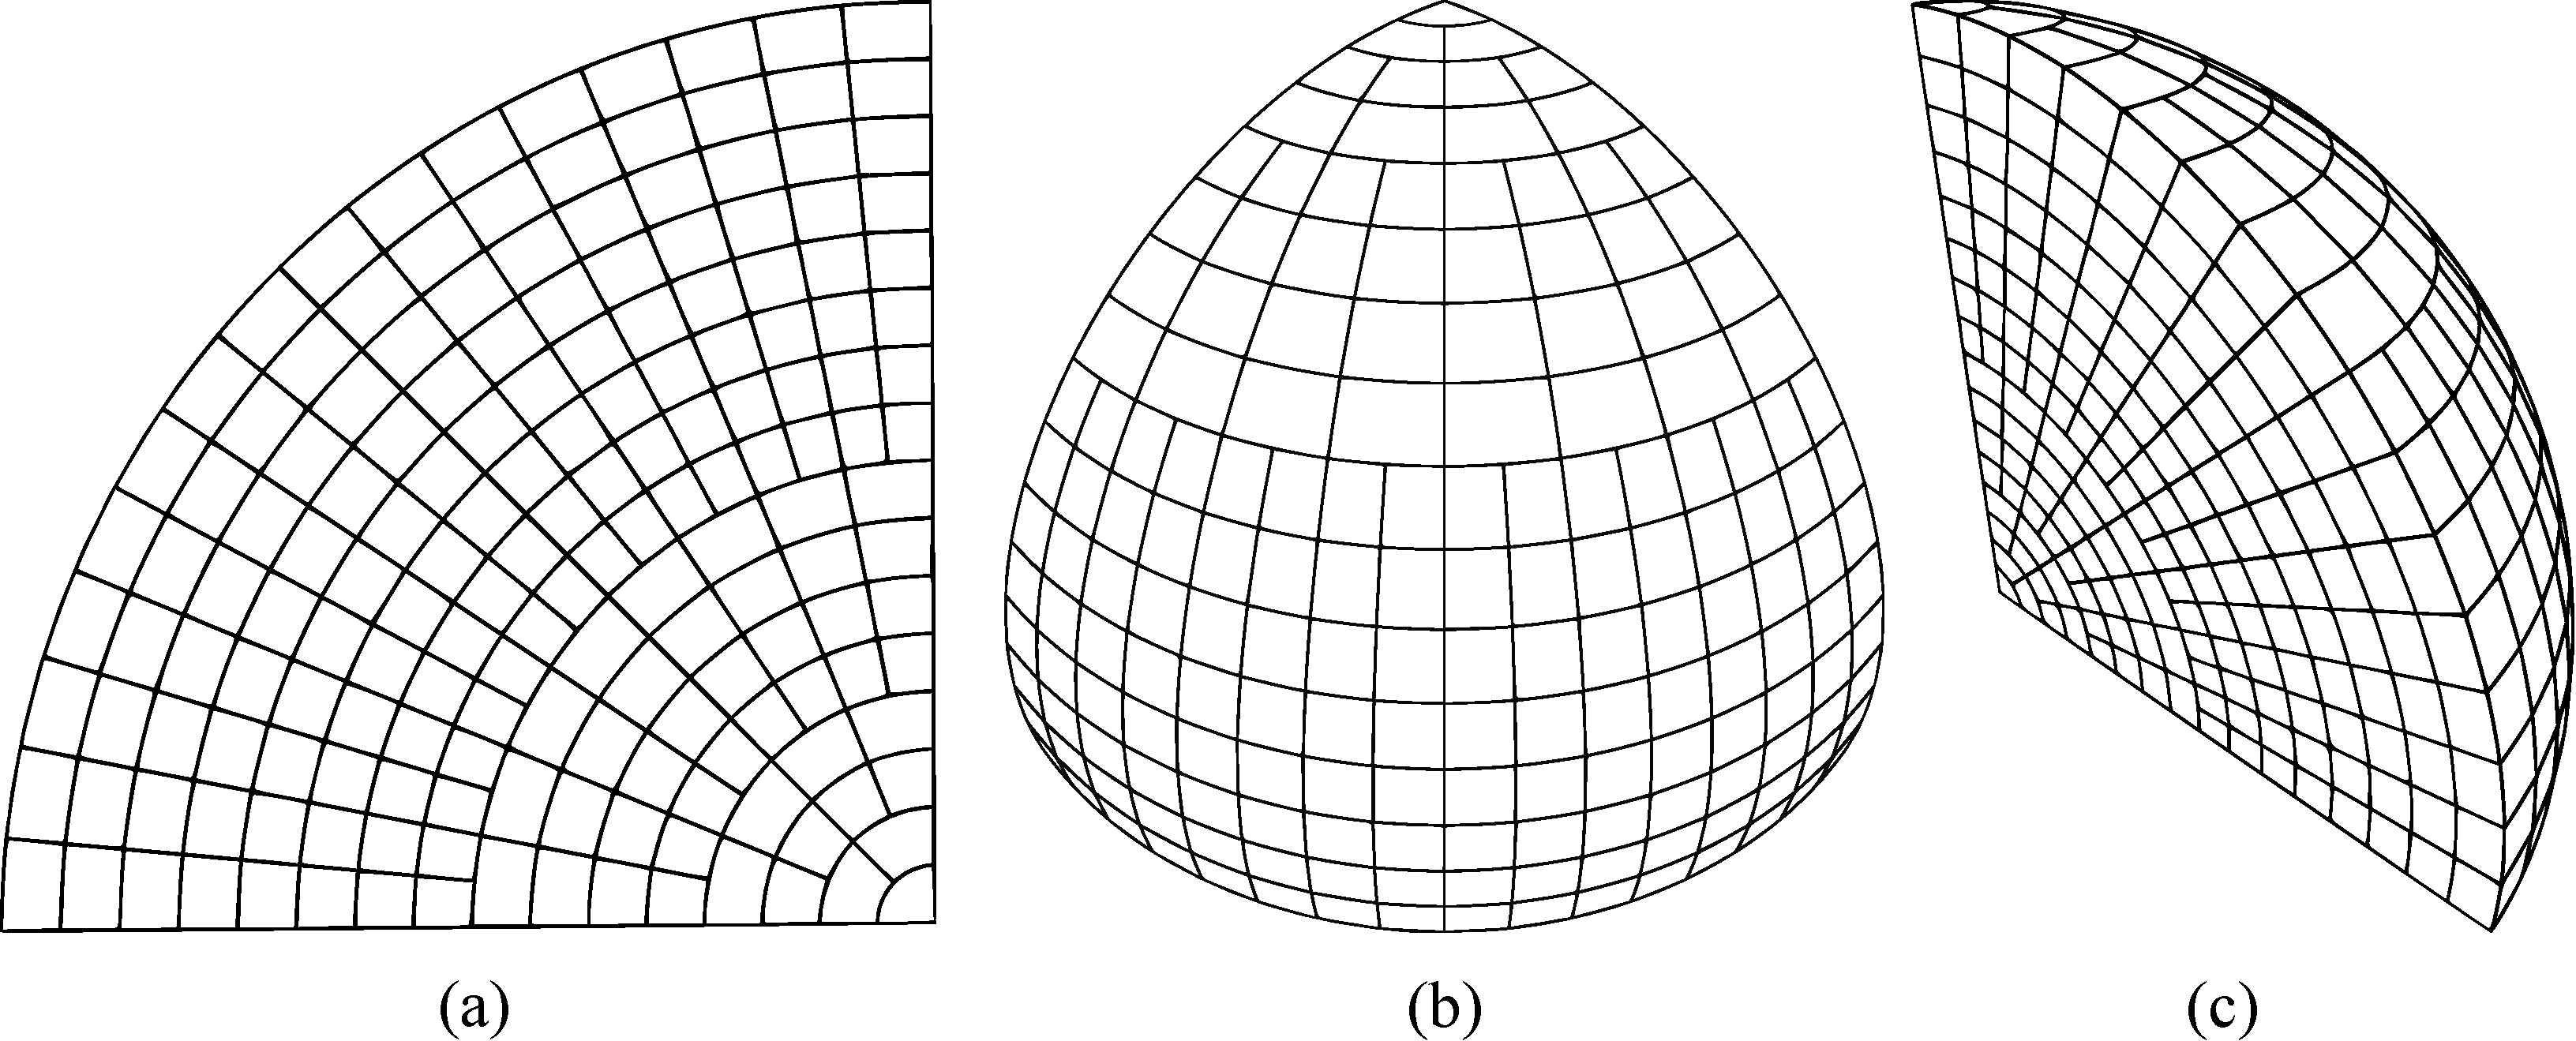
\includegraphics[width=\textwidth]{sdog.pdf}
	\caption[Different views of an SDOG octant]{
		One octant of an SDOG grid after four levels of refinement viewed (a) from the side, (b) from the front, and (c) at an angle.
		Compared to a 3D LLG, cells are more uniform in size and have better compactness.
		Refer to Chapter~\ref{chap:4:results} for a detailed analysis of the volume and compactness properties of SDOG
	}
	\label{fig:sdog}
\end{figure}


\begin{figure}[ht!]
	\centering
	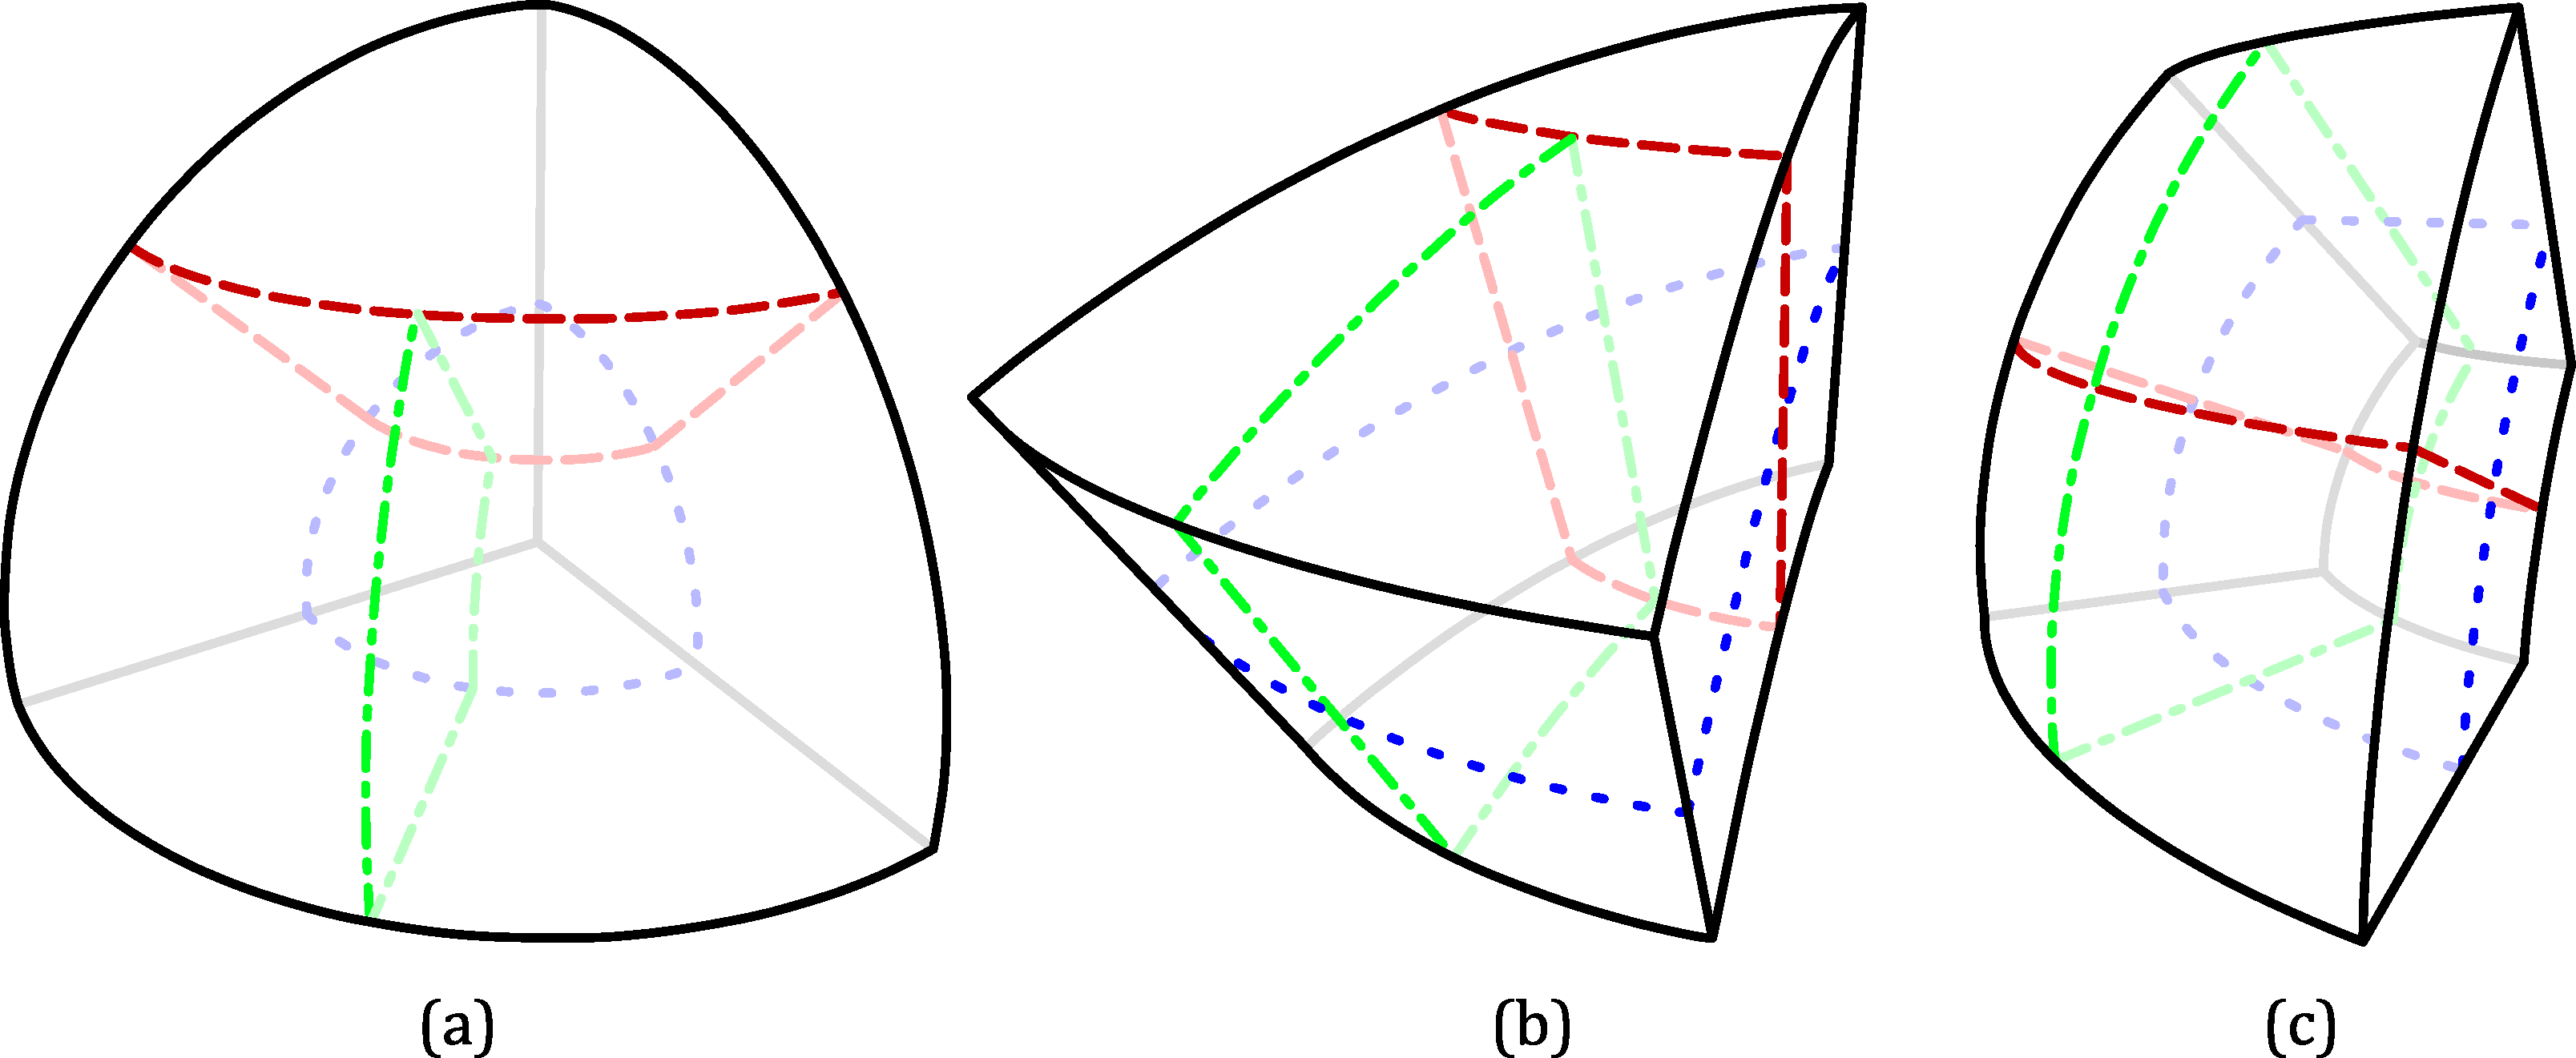
\includegraphics[width=\textwidth]{sdog-refinement.pdf}
	\caption[Splitting surfaces used in SDOG refinement]{
		Location and extent of splitting surfaces in SDOG refinement for (a) SG cells, (b) LG cells, and (c) NG cells.
		Only NG cells have all three splitting surfaces fully refine the cell into eight children, and make up the majority of cells as the grid becomes increasingly refined
	}
	\label{fig:sdog-refinement}
\end{figure}


SDOG cells---including octants---are refined using the midpoint of each spherical coordinate: latitude, longitude, and radius.
These midpoints create splitting surfaces used to split parent cells into smaller children cells.
As described in Chapter~\ref{chap:3:semiregDegen}, a semiregular degenerate refinement is used to prevent excessive degeneration in cell size and compactness near the poles and centre of the sphere.
As a result, SDOG cells are grouped into three classes, depending on which singularities they border.
Figure~\ref{fig:sdog-refinement} shows the resulting splitting surfaces for each type of SDOG cell.


Cells that extend to the centre of the sphere and one of the poles are referred to as Sphere-degenerated Grid (SG) cells (Figure~\ref{fig:sdog-refinement}a) and include the original eight octants.
For these cells, the longitudinal splitting surface does not extend beyond the latitudinal one in the direction towards the pole.
Additionally, neither the latitudinal nor longitudinal splitting surfaces extend beyond the radial one in the direction towards the centre of the sphere.
The result of this refinement is four children cells: another SG cell, one Latitude-degenerated Grid (LG) cell, and two Normal Grid (NG) cells.
We describe LG and NG cells below.
%Only the longitudinal splitting surface for SG cells is symmetric.


LG cells (Figure~\ref{fig:sdog-refinement}b) are similar to SG ones, except that they only extend to one of the poles and not the centre of the sphere.
Therefore, the longitudinal splitting surface does not extend beyond the latitudinal one in the direction towards the pole.
This refinement results in six children cells: two LG cells and four NG cells.


NG cells (Figure~\ref{fig:sdog-refinement}c) extend to neither the pole nor the centre of the sphere and make up the majority of SDOG cells.
These cells are fully refined into eight children NG cells and are the regular case for SDOG refinement.


\subsection{Number of SDOG Cells} \label{chap:4:numCells}
Being able to analyze the number of cells in the grid at each level of refinement is useful not only for measuring volume-preserving properties---such as quickly calculating the average cell volume---but also for analyzing the behaviour of the grid as the level of refinement increases.
This type of analysis will prove useful in informing decisions about how to modify refinement to improve volume preservation.


Due to the degenerate nature of SDOG refinement, calculating the number of cells in the grid is more complicated than a simple exponential formulation.
Despite this, we can use the above refinement rules to derive recursive definitions for the number of cells in an SDOG grid (or a single octant) at a given level of refinement.
Let $S(k)$, $L(k)$, $N(k)$, and $T(k)$ be the number of SG, LG, NG, and total cells of an SDOG octant at refinement level $k$, respectively.
There is only ever one SG cell in an SDOG octant, so trivially
%
\begin{equation*}
S(k) = 1.
\end{equation*}
%
We know each LG cell produces two new LG cells, and that the SG cell produces one new LG cell.
From this we say
%
\begin{equation*}
L(k) = 2L(k-1) + 1 \quad\text{and}\quad L(1) = 1.
\end{equation*}
%
Similarly, each NG cell produces eight new NG cells, each LG cell produces four, and the SG cell produces two.
Thus
%
\begin{equation*}
N(k) = 8N(k-1) + 4L(k-1) + 2 \quad\text{and}\quad N(1) = 2.
\end{equation*}
%
$L(k)$ is a linear non-homogeneous recurrence which can be solved with standard techniques \cite{bellman1963differential}.
Solving and substituting into $N(k)$ we get another linear non-homogeneous recurrence which can be solved similarly.
Finally, we get the closed forms:
%
\begin{equation*}
L(k) = 2^{k} - 1,
\end{equation*}
%
\begin{equation*}
N(k) = \frac{1}{21} \left( 7*2^{k} + 8^{k+1} + 6 \right) - 2^{k}, \quad\text{and}
\end{equation*}
%
\begin{equation*}
T(k) = S(k) + L(k) + N(k) = \frac{1}{21} \left( 7*2^{k} + 8^{k+1} + 6 \right).
\end{equation*}
%
As far as we are aware, these formulations have not been provided in any of the preexisting literature on SDOG.


\subsection{Geometry of SDOG Cells} \label{chap:4:geom}
In order to measure the volume preservation properties of SDOG and its modifications, it is necessary to be able to measure the volume of individual cells in the grid.
Since each SDOG cell represents a range of each spherical coordinate (latitude $\phi$, longitude $\lambda$, and radius $r$), calculating the volume of an individual cell is a straightforward task.
Note that we use the geographic convention for spherical coordinates in this thesis.
Let the subscripts $\mathrm{max}$ and $\mathrm{min}$ denote the maximum and minimum of a given spherical coordinate for an SDOG cell; then, the volume is \cite{yu2009sdog}
%
\begin{equation} \label{eq:volume}
V = \frac{1}{3} \left( \lambda_\mathrm{max} - \lambda_\mathrm{min} \right) \left(r_\mathrm{max}^{3} - r_\mathrm{min}^{3} \right) \left(\sin\phi_\mathrm{max} - \sin\phi_\mathrm{min} \right).
\end{equation}


In addition to the volume of a cell, surface area is another useful property to be able to measure.
Combined with the volume of cells, this allows us to measure the compactness of cells, which we use in Chapter~\ref{chap:4:results} to help evaluate the consequences of our modifications.
From the fact that SDOG cells are refined using spherical coordinates, each face of a cell is a section of a simple geometric shape.
Faces created by radial splitting surfaces are spherical, with surface area given by
%
\begin{equation*}
r^2 \left( \lambda_\mathrm{max} - \lambda_\mathrm{min} \right) \left( \sin\phi_\mathrm{max} - \sin\phi_\mathrm{min} \right).
\end{equation*}
%
Faces created by longitudinal splitting surfaces are the difference of two circular sectors, and have an area of
%
\begin{equation*}
\frac{1}{2} \left( \phi_\mathrm{max} - \phi_\mathrm{min} \right) \left( r_\mathrm{max}^{2} - r_\mathrm{min}^{2} \right).
\end{equation*}
%
Finally, faces created by latitudinal splitting surfaces lie on a cone, with a surface area of
%
\begin{equation*}
\frac{1}{2} \cos\phi \left( \lambda_\mathrm{max} - \lambda_\mathrm{min} \right) \left( r_\mathrm{max}^{2} - r_\mathrm{min}^{2} \right).
\end{equation*}


\section{Modified SDOG Refinement} \label{chap:4:modified}
The main goal of this work is to modify SDOG in such a way as to improve volume preservation while minimizing the impact on other desired properties of the grid.
As a baseline, the distribution of cell volumes in a conventional SDOG grid is visualized in Figure~\ref{fig:sdog-volume}.
In conventional SDOG refinement, the location of the different splitting surfaces is always at the midpoint of the respective spherical coordinate; we question if this should be the case.
For an octree in Euclidean space, this type of refinement is desirable, as it generates children cells of identical size and shape.
In spherical space, however, this property does not transfer.
Using midpoints to refine cells makes for a simple refinement scheme, but it makes no guarantees about the shape or size of the resulting child cells.


\begin{figure}[ht!]
	\centering
	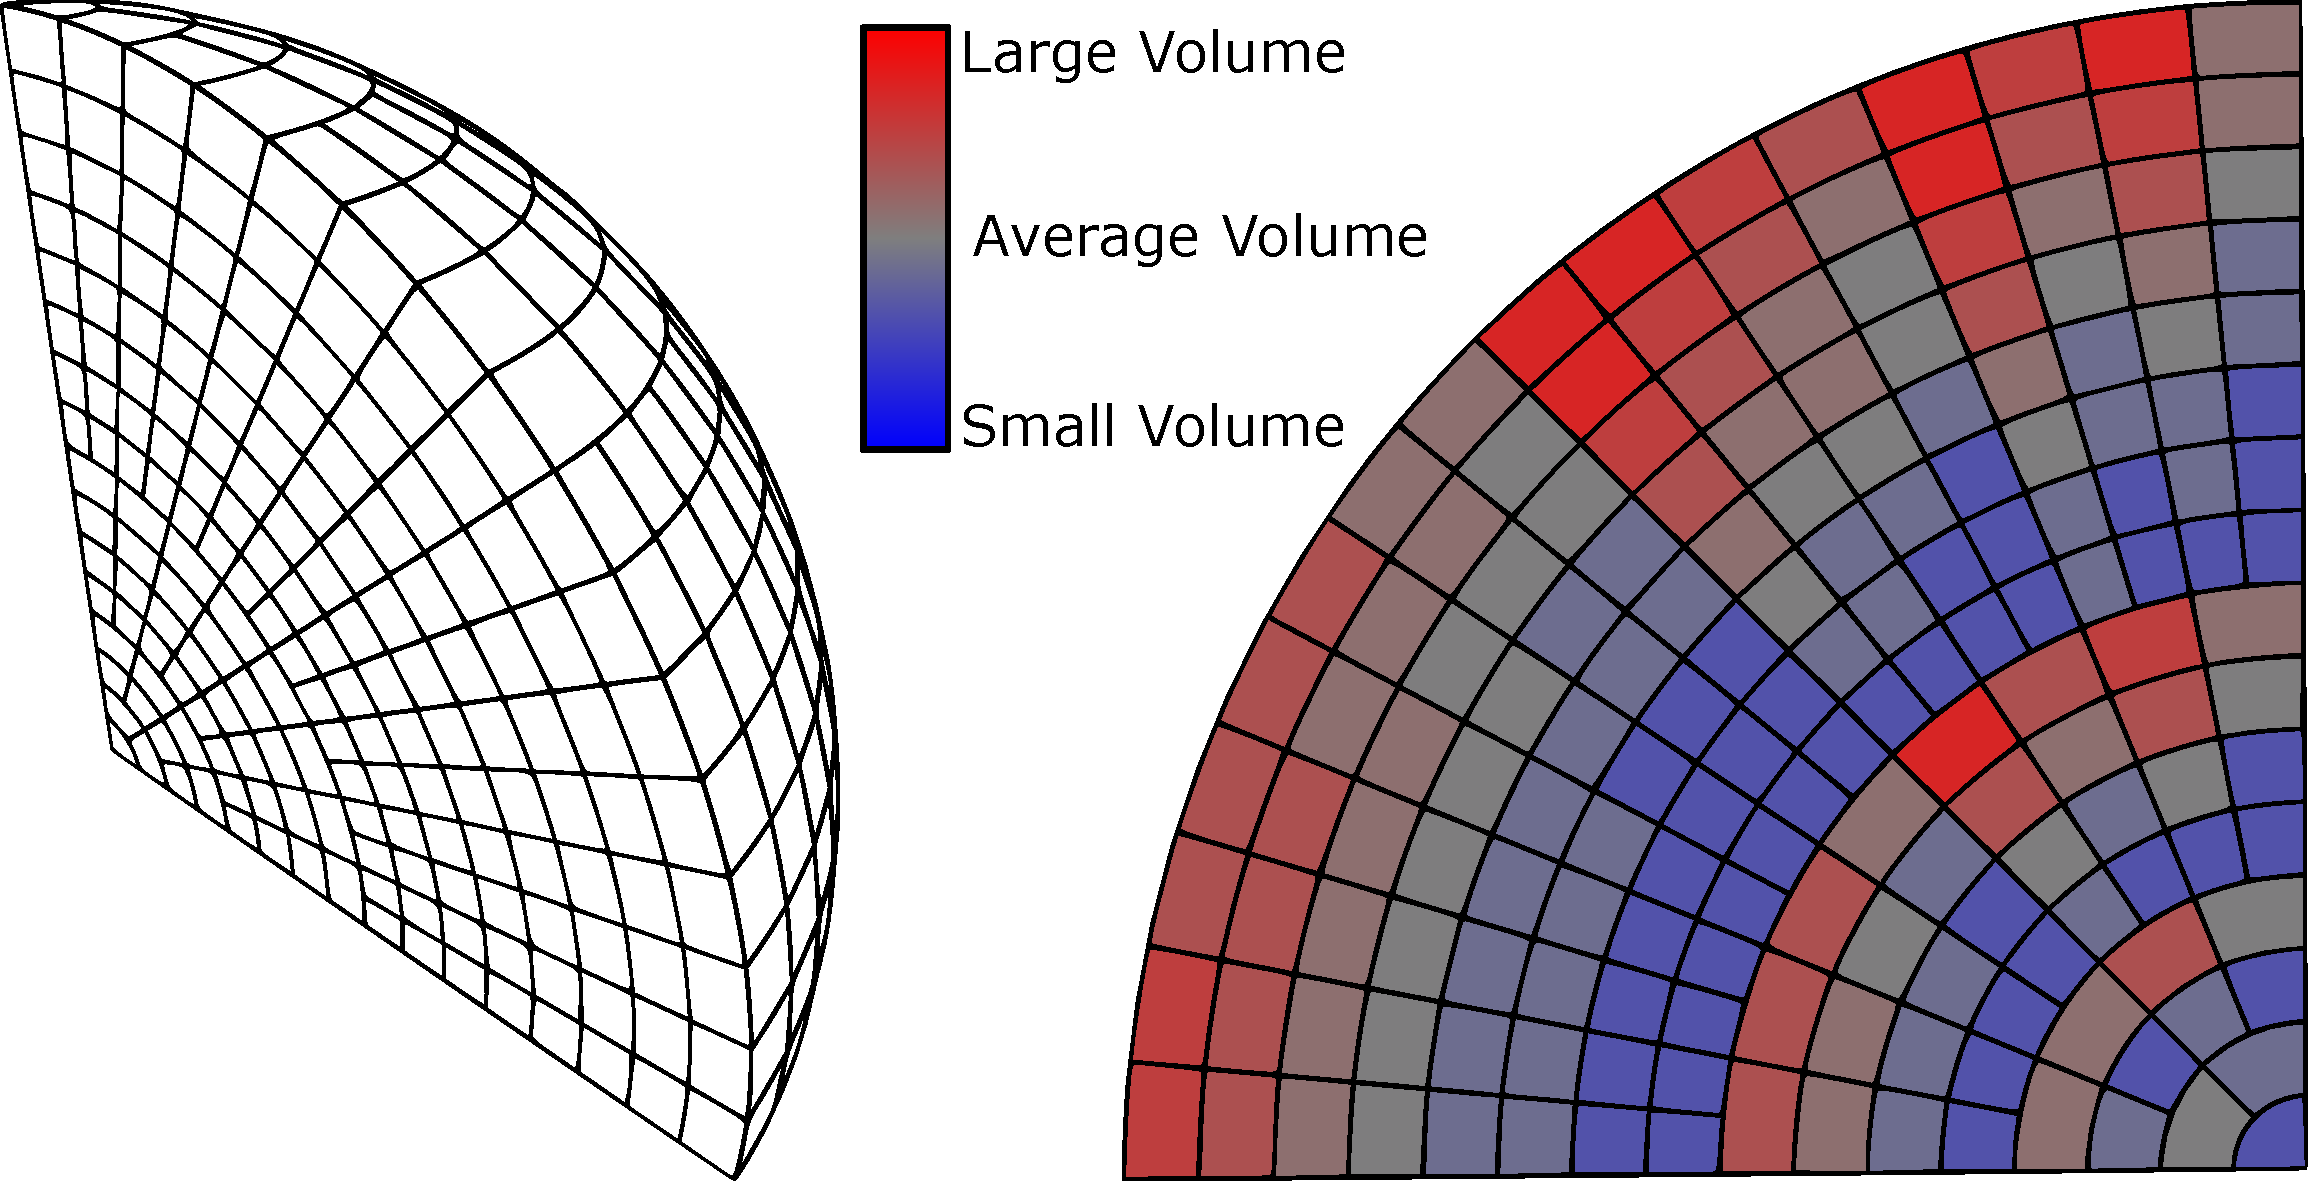
\includegraphics[width=0.85\textwidth]{sdog-volume.pdf}
	\caption[Distribution of cell volumes in SDOG]{
		Distribution of cell volumes in an octant after four levels of conventional SDOG refinement
	}
	\label{fig:sdog-volume}
\end{figure}


\begin{figure}[ht!]
	\centering
	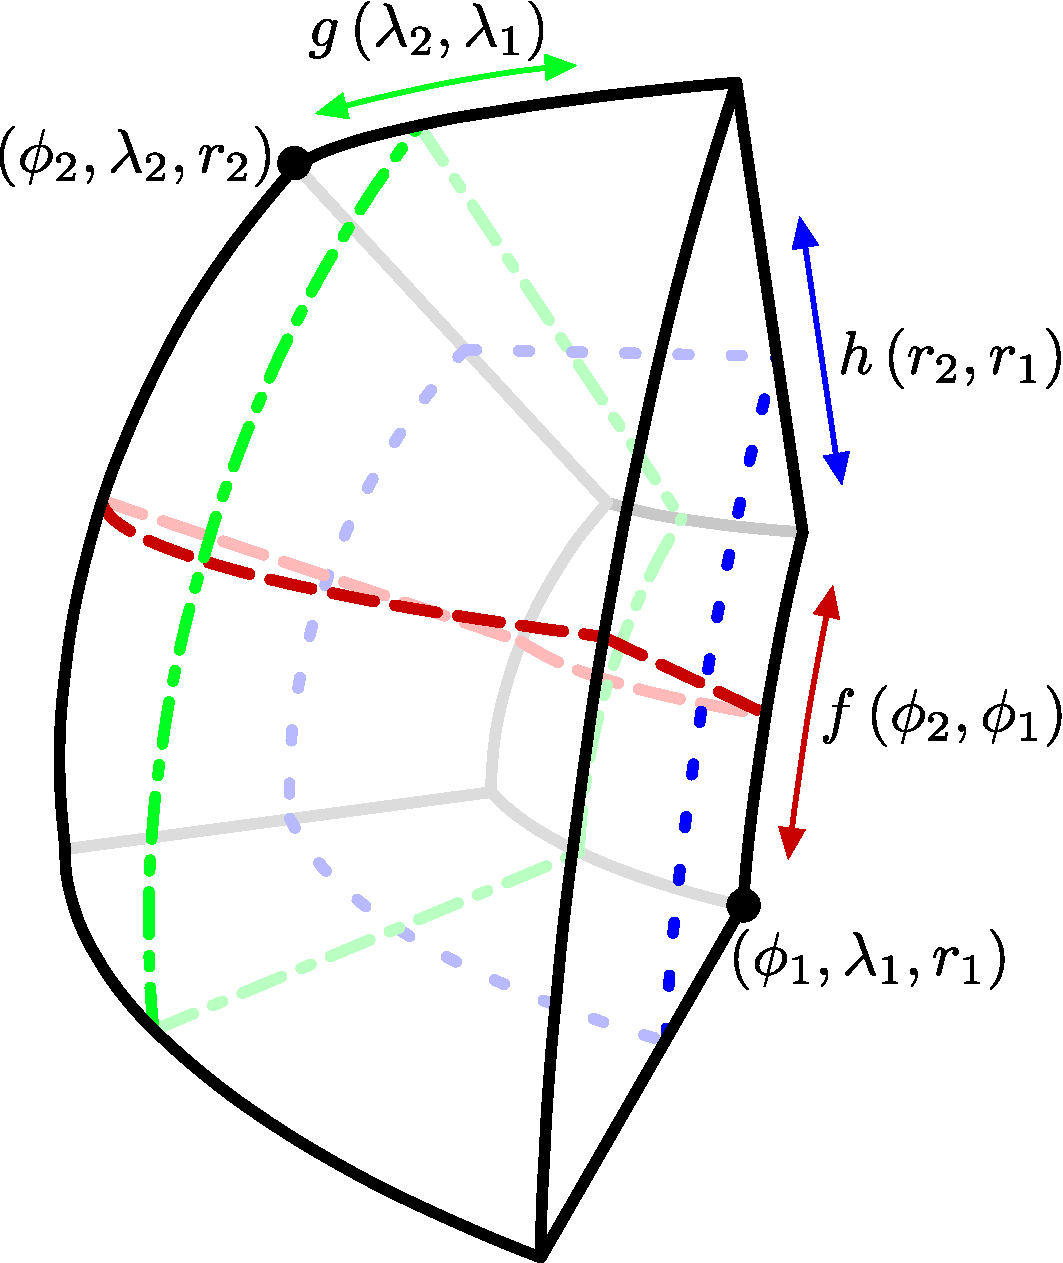
\includegraphics[width=0.4\textwidth]{sdog-functions.pdf}
	\caption[How functions determine the location of SDOG splitting surfaces]{
		Each SDGO cell represents a range in each spherical coordinate; the location of the splitting surfaces is expressed as a function of the maximum and minimum of the respective range.
		Here we show only an NG cell; however, the same applies to SG and LG cells.
		The functions $f$, $g$, and $h$ serve as placeholders for any valid function that results in the output being strictly between the two inputs
	}
	\label{fig:functions}
\end{figure}


By allowing the location of the splitting surfaces to be adjusted, we can modify the shape and size of child cells and as a result affect the volume preservation, compactness, and other properties of the grid.
Let $c_{s}$ be the location of the splitting surface, where $c$ is one of $\left\lbrace \phi, \lambda, r \right\rbrace$.
One way to express the location of the splitting surfaces used for refinement is as a convex combination of maximum and minimum values:
%
\begin{equation*}
c_{s} = \alpha c_\mathrm{max} + \left( 1-\alpha \right) c_\mathrm{min}, \quad \alpha \in \left( 0, 1 \right),
\end{equation*}
%
where we call $\alpha$ the splitting factor.
Conventional SDOG used midpoints (i.e. $\alpha = 1/2$) for each spherical coordinate during refinement, regardless of cell type.
While a convex combination is the most straightforward, any function of the maximum and minimum such that the result is strictly between the two is a valid method for determining the location of the splitting surfaces (Figure~\ref{fig:functions}).
Thus, the location of splitting surfaces is modified by changing this function, either by using a different value of $\alpha$ or by using a different function altogether.
Furthermore, the function used can be different for each cell type and spherical coordinate.


A useful function for improving volume preservation is one that results in one of the new ranges having a specific percentage of the volume of the original range.
We start with the radial splitting surface.
Referring to Equation~(\ref{eq:volume}), let $p \in (0,1)$ be the percentage we wish for the lower range to have, then
%
\begin{equation*}
p \left( r_\mathrm{max}^{3} - r_\mathrm{min}^{3} \right) = r_{s}^{3} - r_\mathrm{min}^{3}
\end{equation*}
%
\begin{equation*}
p r_\mathrm{max}^{3} - p r_\mathrm{min}^{3} = r_{s}^{3} - r_\mathrm{min}^{3}
\end{equation*}
%
\begin{equation*}
r_{s}^{3} = p r_\mathrm{max}^{3} + r_\mathrm{min}^{3} - p r_\mathrm{min}^{3}
\end{equation*}
%
\begin{equation*}
r_{s}^{3} = p r_\mathrm{max}^{3} + \left( 1 - p \right) r_\mathrm{min}^{3}
\end{equation*}
%
\begin{equation} \label{eq:radVol}
r_{s} = \sqrt[3]{ p r_\mathrm{max}^{3} + \left( 1 - p \right) r_\mathrm{min}^{3} }.
\end{equation}
%
The derivations for the latitudinal and longitudinal splitting surfaces follow the same, with results
%
\begin{equation} \label{eq:latVol}
\phi_{s} = \sin^{-1} \left( p \sin\phi_\mathrm{max} + \left( 1 - p \right) \sin\phi_\mathrm{min} \right) \quad\text{and}
\end{equation}
%
\begin{equation} \label{eq:longVol}
\lambda_{s} = p \lambda_\mathrm{max} + \left( 1 - p \right) \lambda_\mathrm{min}.
\end{equation}


The question then becomes which splitting surfaces should be modified, and in which ways, in order to improve the volume preservation of the grid.
We first look at which splitting surfaces should \textit{not} be modified.
From Equation~(\ref{eq:longVol}), it is clear a longitudinal splitting surface at the midpoint will always split a cell exactly in half, and therefore they should not be changed.


\begin{figure}[ht!]
	\centering
	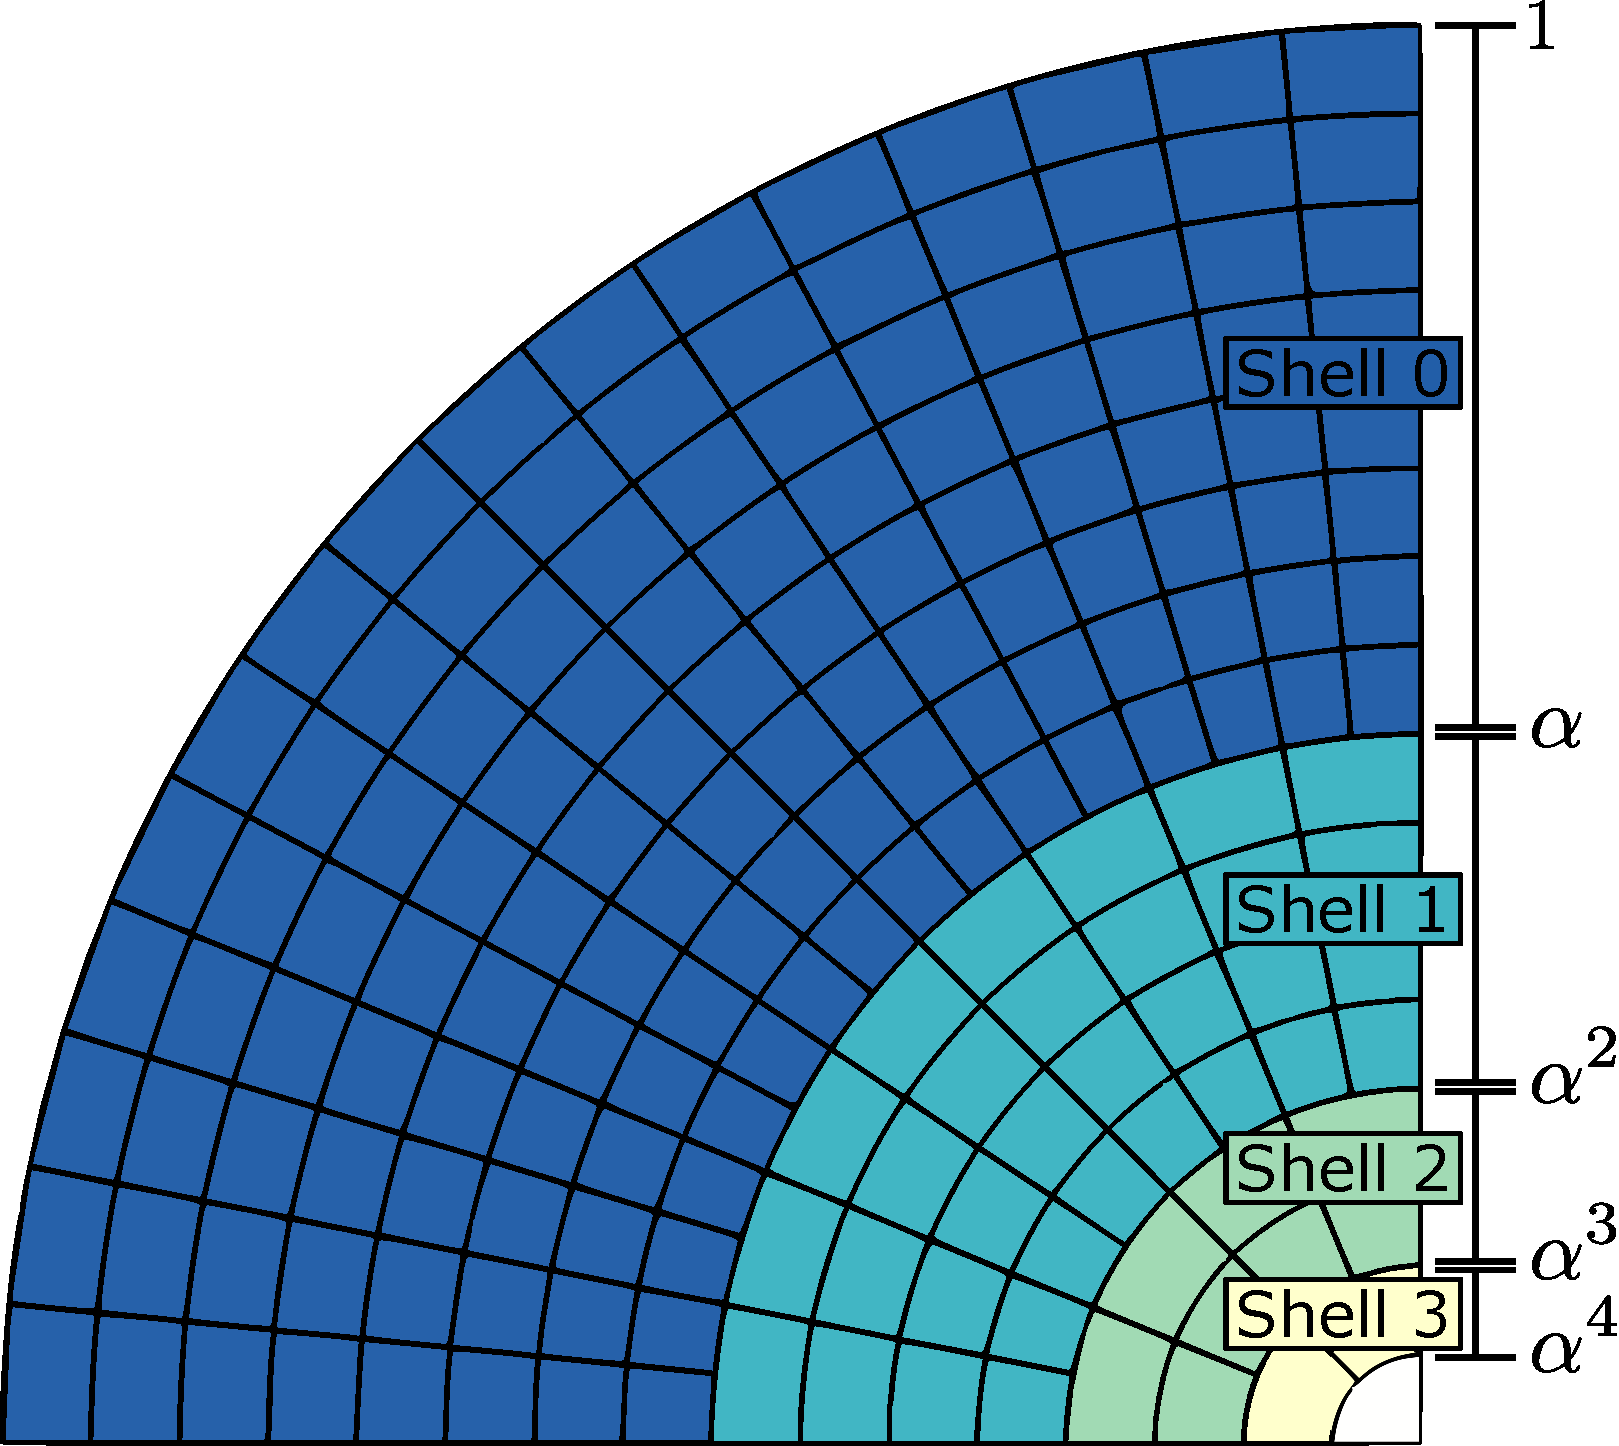
\includegraphics[width=0.6\textwidth]{sdog-shells.pdf}
	\caption[Spherical shells that result from SDOG refinement]{
		Spherical shells created by the radial splitting surfaces of SG cells.
		At $k$ levels of refinement there are $k$ shells and one inner SG cell.
		These shells are similar and should have volume proportional to the number of cells they contain
	}
	\label{fig:sdog-shells}
\end{figure}


Less trivially, the radial splitting surface for SG cells should also be left at the midpoint.
Referring to Figure~\ref{fig:sdog-shells}, we see that the radial splitting surfaces for SG cells separate the grid into spherical shells.
Shell $n$ has a volume proportional to
%
\begin{equation*}
\alpha^{3n} - \alpha^{3 \left( n + 1 \right)},
\end{equation*}
%
so the ratio of the volumes of shell $n+1$ and $n$ is
%
\begin{equation*}
\frac{ \alpha^{3 \left(n + 1 \right)} - \alpha^{3\left( n + 2 \right)} }{ \alpha^{3n} - \alpha^{3 \left( n + 1 \right)} } = \frac{ \alpha^{3} \alpha^{3n} \left( 1 - \alpha^{3} \right) }{ \alpha^{3n} \left( 1 - \alpha^{3} \right) } = \alpha^{3}.
\end{equation*}
%
From the self similar nature of SDOG refinement, we know that the cells in shell $n$ are simply the cells of shell $n+1$ refined once.
We also know that, in the limit, an SDOG grid at one level higher of refinement will have eight times as many cells as the previous resolution ($\lim_{k \to \infty} T(k+1) / T(k)  = 8 $).
Therefore, in order for cells in the grid to be close to equal volume, it must be that shell $n+1$ has one eighth the volume of shell $n$---since it will have one eighth the number of cells---which occurs exactly when $\alpha = 1 / 2$.


We are left with five possible splitting surfaces to be modified: the radial splitting surface for LG and NG cells, and the latitudinal splitting surface for SG, LG, and NG cells.
Below, we determine the ideal placement for each of these surfaces to maximize volume preservation between cells.
We then propose other possible splitting surface combinations to balance the tradeoff between volume preservation and cell compactness.


\subsection{Ideal Splitting Surfaces for Volume Preservation} \label{chap:4:ideal}
Ideal splitting surfaces to maximize volume preservation are achieved using Equations~(\ref{eq:radVol}) and (\ref{eq:latVol}); all that is required is to determine the ideal value of $p$ for the different splitting surfaces and cell types.
We start with the radial splitting surfaces for LG and NG cells, and the latitudinal one for NG cells, as these surfaces behave the same as regular refinement.
Specifically, these splitting surfaces result in the same number and type of cells on both sides, a property that also holds for their children.
We call these the regular splitting surfaces.
Therefore, we require that the volume on each side of the regular splitting surfaces be equal, or in other words, we set $p = 1/2$ for these splitting surfaces.


\begin{figure}[ht!]
	\centering
	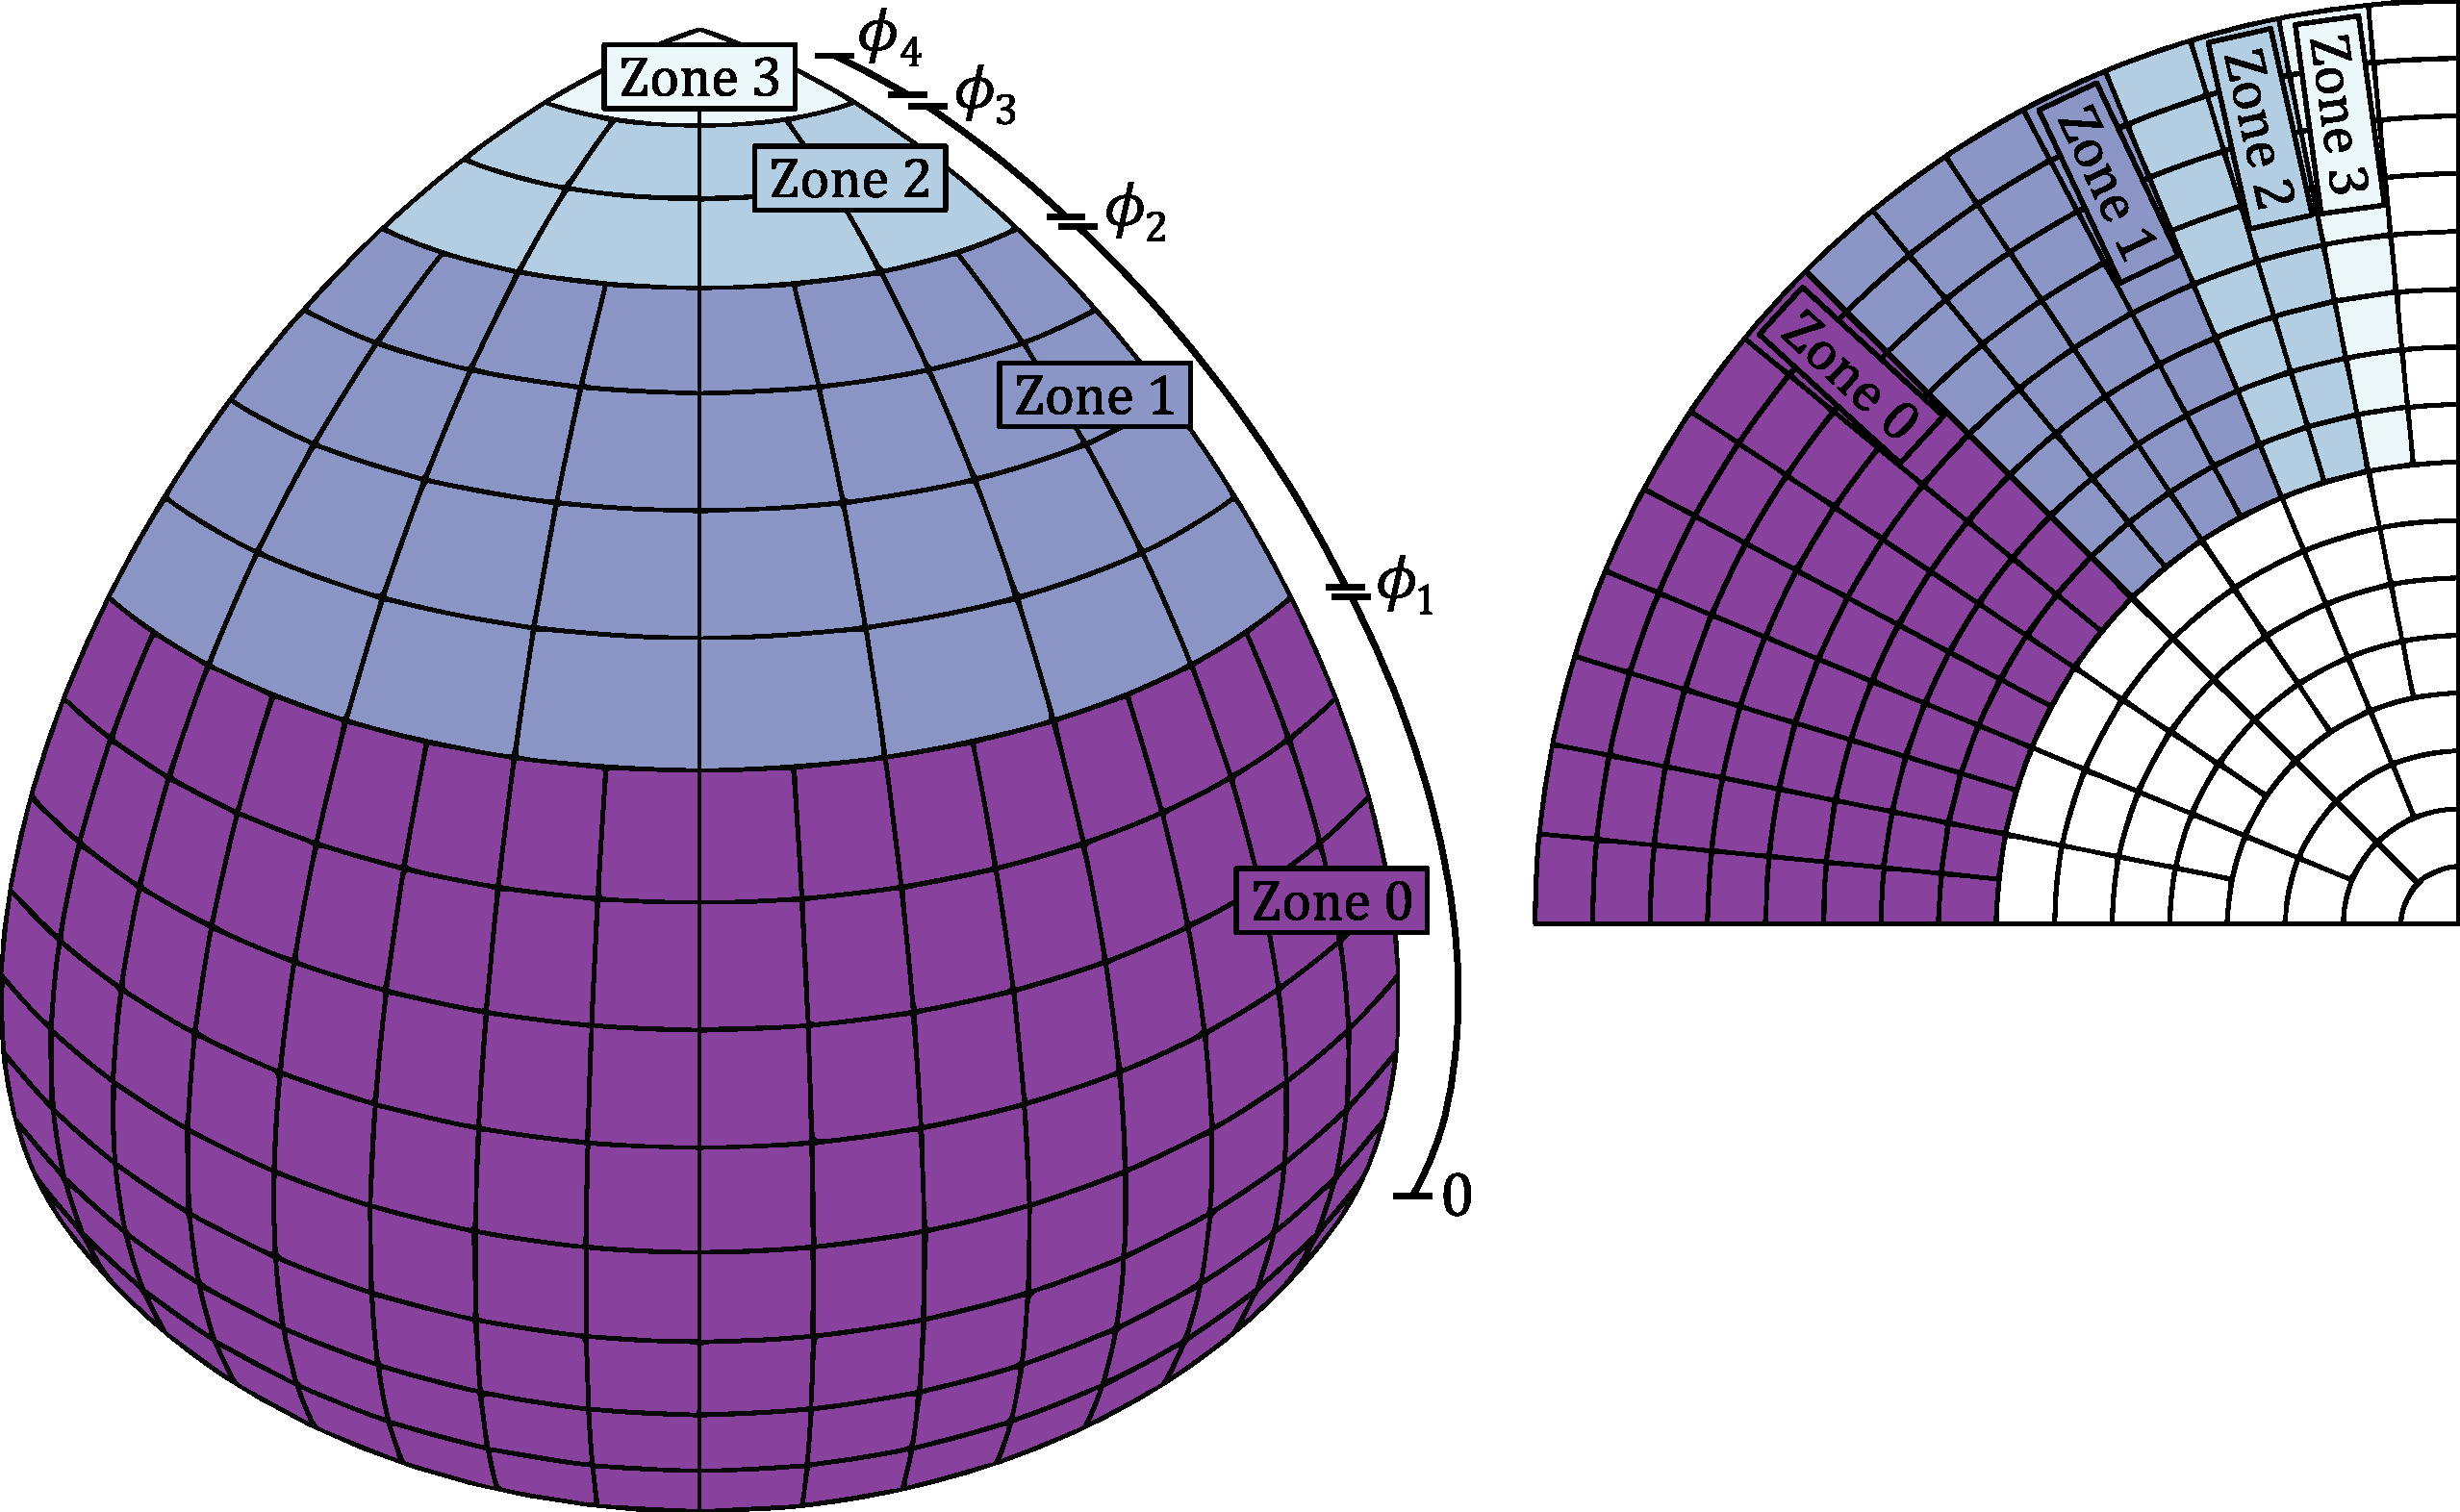
\includegraphics[width=0.9859\textwidth]{sdog-zones.pdf}
	\caption[Spherical zones that result from SDOG refinement]{
		Spherical zones created by the latitudinal splitting surfaces of SG and LG cells.
		At $k$ levels of refinement, there are $k$ zones and one upper stack of LG cells in the outermost shell.
		Each successively smaller shell has one fewer zone than the previous until reaching the innermost SG cell.
		Zones in the same shell are not exactly similar, but are regular grid regions and should have volume proportional to the number of cells they contain
	}
	\label{fig:sdog-zones}
\end{figure}


Determining the ideal latitudinal splitting surfaces for SG and LG cells is more involved.
First, notice that these two latitudinal splitting surfaces have a similar effect as the radial splitting surface for SG cells.
Referring to Figure~\ref{fig:sdog-zones}, we see that these splitting surfaces further divide the spherical shells into spherical zones.
Additionally, each zone is comprised entirely of NG cells.
From this, we conclude that zone $n$ has precisely four times as many cells as zone $n+1$, and thus, should have four times the volume as well.
Using this information, we find the value for $p$.
Zone $n$ has a volume equal to $\left( 1 - p \right)^{n} p$ that of the initial octant, then setting the ratio between zone $n+1$ and $n$ to be equal to $1/4$ gives us $p = 3/4$.


\begin{figure}[ht!]
	\centering
	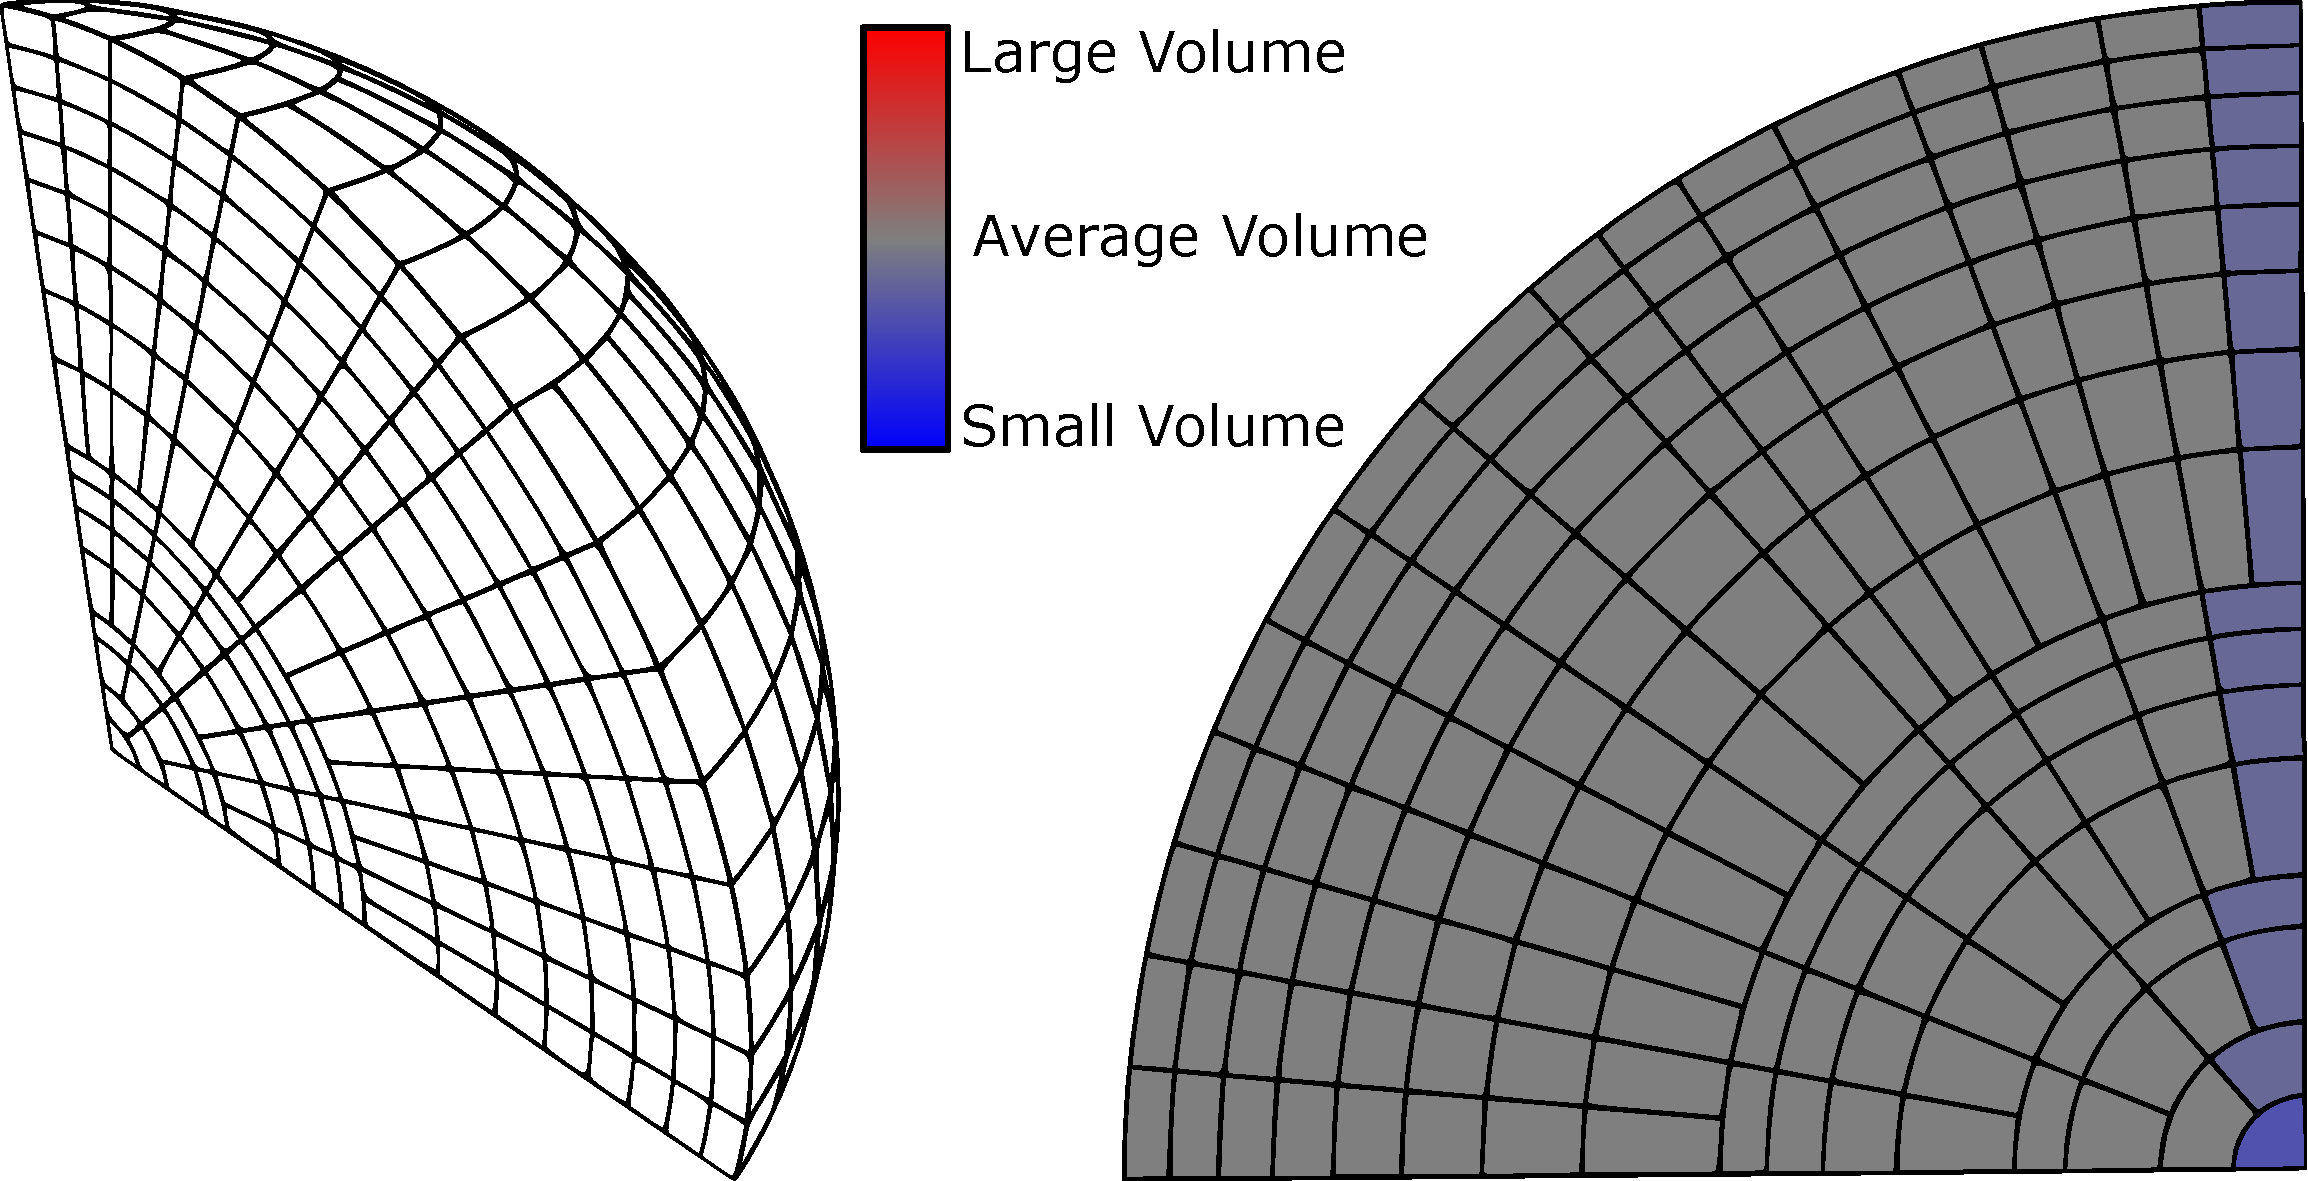
\includegraphics[width=0.85\textwidth]{modified-volume.pdf}
	\caption[Distribution of cell volumes in the volume modification]{
		Results of the volume method after four levels of refinement.
		All NG cells have exactly the same volume, with the LG and SG cells having a lower volume.
		Notice how the resulting NG cells are stretched and squashed in order to ensure they all have equal volume
	}
	\label{fig:modified-volume}
\end{figure}


Figure~\ref{fig:modified-volume} shows the resulting grid from this method of calculating splitting surfaces, which we refer to as the \textit{volume} method.
In this grid, all NG cells at the same level of refinement have equal volume; this dramatically improves the volume preservation, as only cells that extend to one of the singularities (i.e. SG and LG cells) will have a different volume than the other cells in the grid.


\subsection{Balanced Splitting Surfaces} \label{chap:4:balanced}
While the above refinement method significantly improves volume preservation in the grid, this gain does not come without consequence.
Cells are stretched and squashed in order to achieve this volume preservation, which reduces cell compactness and may be an undesirable effect depending on the application.
In order to address this issue, it is possible to use different splitting surfaces that achieve a better balance between volume preservation and cell compactness.


\begin{figure}[ht!]
	\centering
	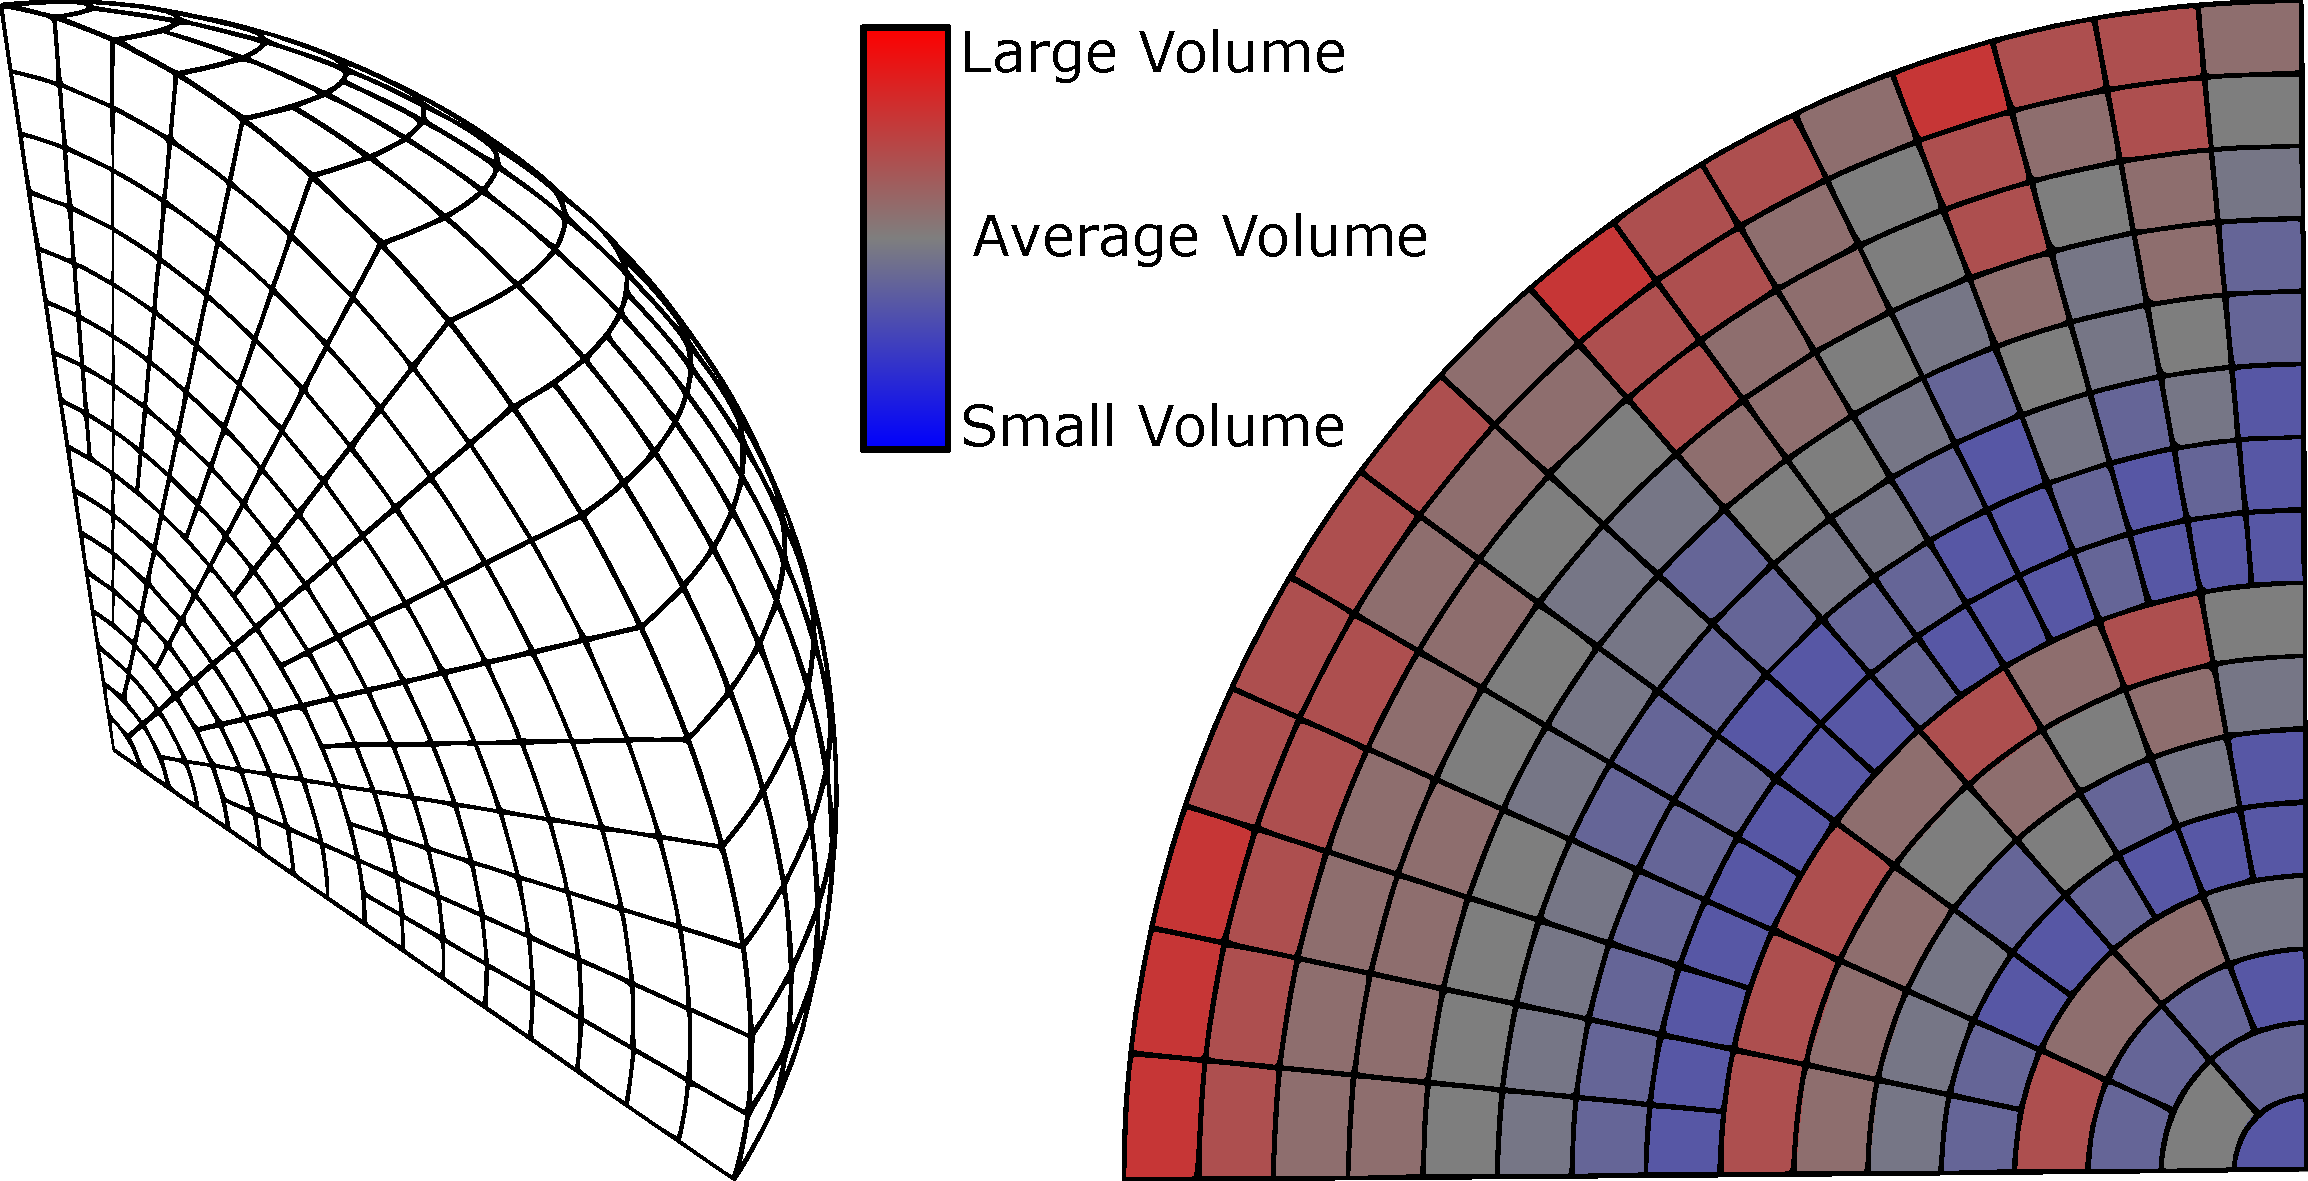
\includegraphics[width=0.85\textwidth]{alpha-volume.pdf}
	\caption[Distribution of cell volumes in the latitude modification]{
		Results of the latitude method after four levels of refinement.
		Since only latitude splitting surface for SG and LG cells have been modified, the results are similar to that of conventional SDOG
	}
	\label{fig:alpha-volume}
\end{figure}


Looking at Figure~\ref{fig:modified-volume}, we see that the regular splitting surfaces are responsible for the majority of the reduction in cell compactness.
Our first balanced scheme then is to leave these splitting surfaces at the midpoints and only modify the latitudinal splitting surfaces for SG and LG cells.
Figure~\ref{fig:alpha-volume} shows the results of this method, which we refer to as the \textit{latitude} method.
Comparing this to conventional SDOG (refer back to Figure~\ref{fig:sdog-volume}), the two grids are nearly identical.
Thus, this method offers only a slight improvement with regards to volume preservation, while also only slightly sacrificing cell compactness.


\begin{figure}[ht!]
	\centering
	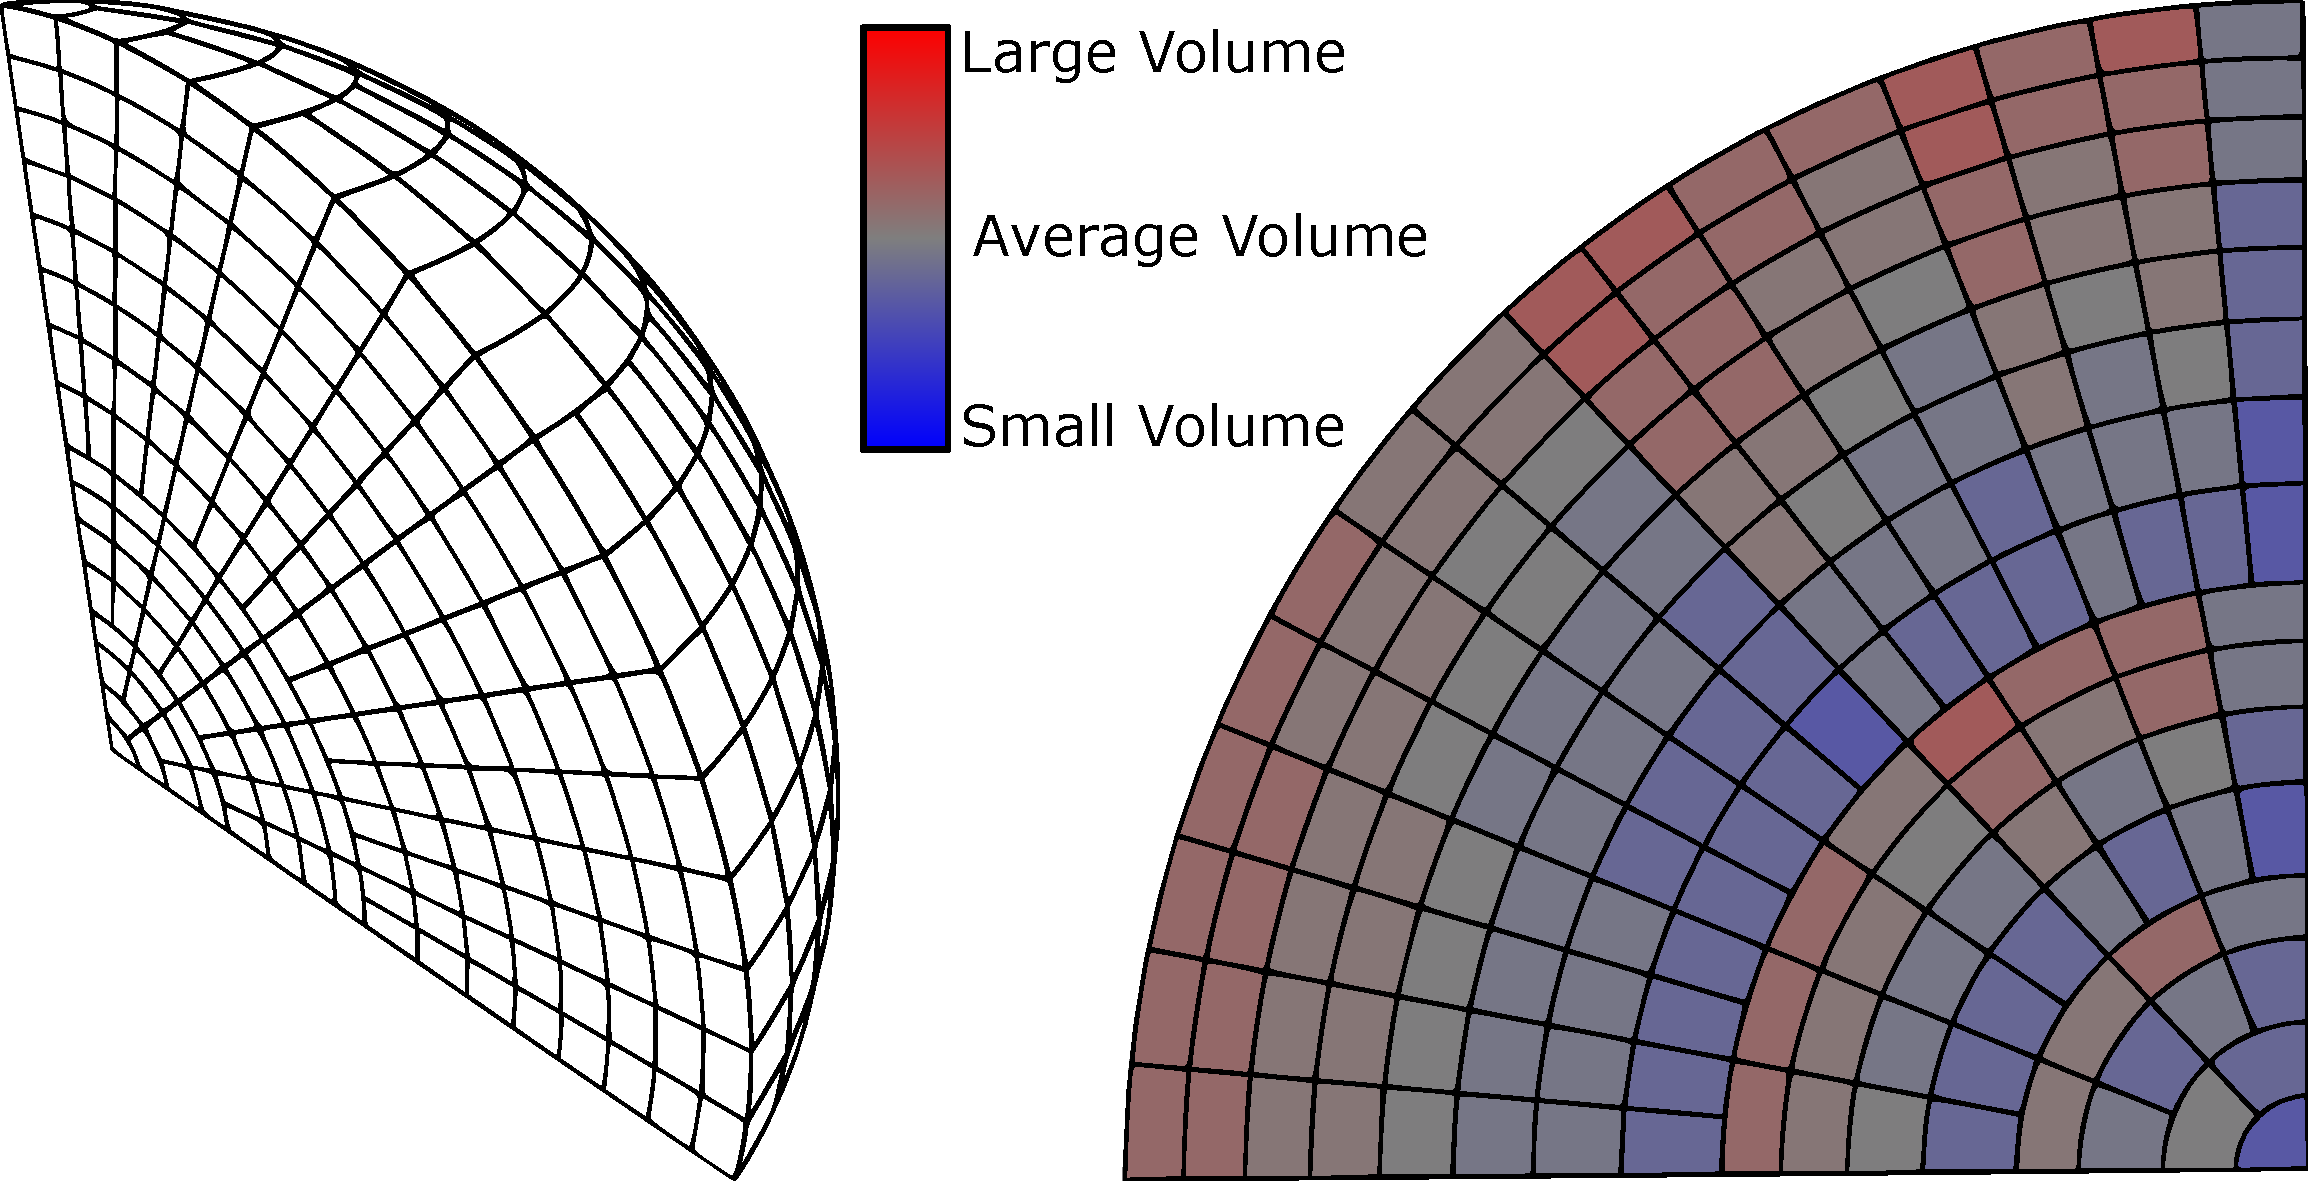
\includegraphics[width=0.85\textwidth]{blend-volume.pdf}
	\caption[Distribution of cell volumes in the balanced modification]{
		Results of the balanced method after four levels of refinement.
		NG cells are still stretched and squashed in order to better preserve volume; however, the effect is less pronounced than in the volume method
	}
	\label{fig:blend-volume}
\end{figure}


In order to achieve different tradeoffs between compactness and volume preservation, modifying the regular splitting surfaces is necessary.
Equations~(\ref{eq:radVol}) and (\ref{eq:latVol}) give ideal placements for volume preservation as compared to the conventional midpoint functions which result in better compactness.
Therefore, using different functions that blend between these two extremes allows for a more balanced tradeoff.
There are endless possibilities for these functions; however, as will be required in Chapter~\ref{chap:mapping}, they should be easily invertible.
That is, given a splitting surface, we need to be able to determine the corresponding value of $p$.
For the radial splitting surfaces, we propose the function
%
\begin{equation*}
r_{s} = \sqrt[t]{ p r_\mathrm{max}^{t} + \left( 1 - p \right) r_\mathrm{min}^{t} }
\end{equation*}
%
where $1 \leq t \leq 3$ blends between compactness at $t = 1$ (equivalent to midpoint) and volume preservation at $t=3$ (equivalent to Equation~(\ref{eq:radVol})).
For the latitudinal splitting surfaces, we propose
%
\begin{equation*}
\phi_{s} = h \sin^{-1} \left( p \sin \left( \frac{1}{h} \phi_\mathrm{max} \right) + \left( 1 - p \right) \sin \left( \frac{1}{h} \phi_\mathrm{min} \right) \right)
\end{equation*}
%
where $1 \leq h \leq \infty$ blends between volume preservation at $h = 1$ (equivalent to Equation~(\ref{eq:latVol})) and compactness at $h = \infty$ (equivalent to midpoint). We found values of $t = 2$ and $h = 1.45$ to offer a relatively balanced tradeoff between the two properties, with the resulting grid shown in Figure~\ref{fig:blend-volume}.
We refer to this method as the \textit{balanced} one.


\section{Results} \label{chap:4:results}
There are several potential methods for evaluating the volume-preserving properties of a 3D DGGS.
When first proposed by Yu and Wu, the ratio between cells of the largest and smallest volume was used to evaluate the volume-preserving properties of SDOG~\cite{yu2009sdog}.
This volume ratio is a useful measure for determining the worst-case difference in the volume of cells; however, it does not give any information about the distribution of said volumes.
For example, a grid with all cells except one having equal volume, and a grid where every cell has a distinct volume, could end up having the same volume ratio.
To get a complete understanding of volume preservation, we should also examine statistics that give a measure of distribution.
For this purpose, we use the coefficient of variation (CV), which is simply the ratio between the standard deviation (SD) and the mean.
We use the CV over the SD as it a dimensionless quantity.


In modifying the refinement for volume preservation, it is also important to evaluate the impact these changes have on other properties of the grid.
Specifically, we should measure the effect our changes have on the compactness of cells.
To measure this, we use the notion of sphericity, which quantifies how closely the shape of an object approximates a sphere~\cite{wadell1935volume}.
Sphericity is defined as the ratio between the surface area of a sphere with the same volume as the object and the surface area of the object itself.
Therefore, a perfect sphere will have a sphericity of one, and any other object will have sphericity strictly less than one.
Formally, given an object $\omega$ and a sphere $s$ such that $\operatorname{vol}(s) = \operatorname{vol}(\omega)$, the sphericity of $\omega$, $\Psi$, is given by $\operatorname{area}(s) / \operatorname{area}(\omega)$ , or equivalently 
%
\begin{equation*}
\Psi = \frac{\pi^{\frac{1}{3}}\left( 6\operatorname{vol}(\omega) \right)^{\frac{2}{3}}}{\operatorname{area}(\omega)}.
\end{equation*}
%
We use the mean and SD of sphericity for all cells in the grid to evaluate compactness globally.

\begin{figure}[p!]
	\centering
	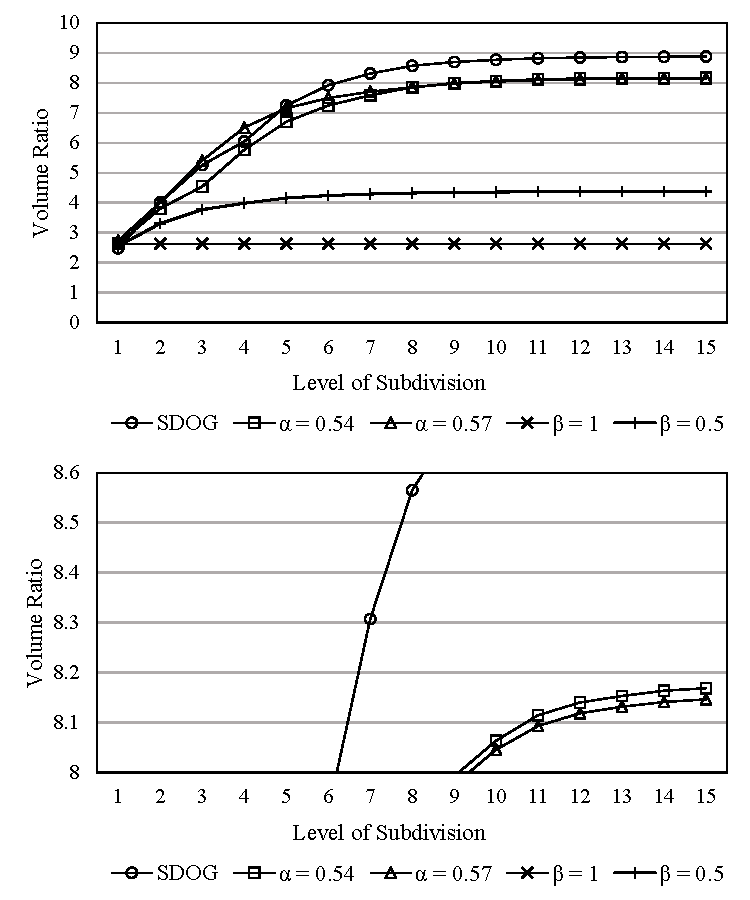
\includegraphics[width=0.8\textwidth]{volume-ratio.pdf}
	\caption[Graph of volume ratio for the different grids]{
		Volume ratio for the different grids at increasing levels of refinement.
		Note that for the volume method, the volume ratio does not change with refinement level
	}
	\label{fig:vr}
\end{figure}


\begin{figure}[p!]
	\centering
	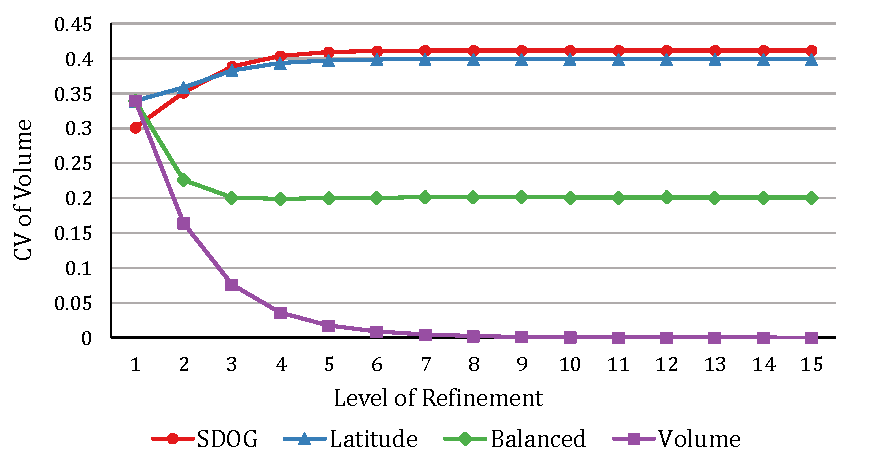
\includegraphics[width=0.8\textwidth]{cv-volume.pdf}
	\caption[Graph of CV of volume for the different grids]{
		CV of volume for the different grids at increasing levels of refinement
	}
	\label{fig:cv}
\end{figure}


\begin{figure}[p!]
	\centering
	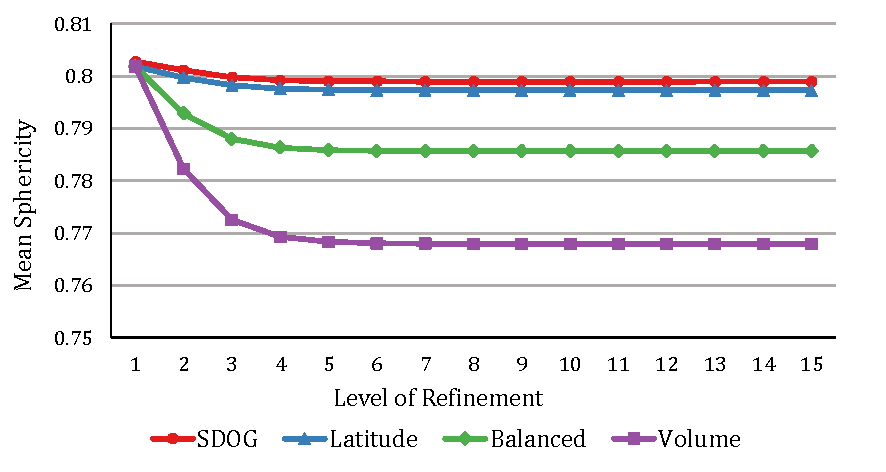
\includegraphics[width=0.8\textwidth]{mean-sph.pdf}
	\caption[Graph of mean sphericity for the different grids]{
		Mean sphericity for the different grids at increasing levels of refinement
	}
	\label{fig:sph}
\end{figure}


\begin{figure}[p!]
	\centering
	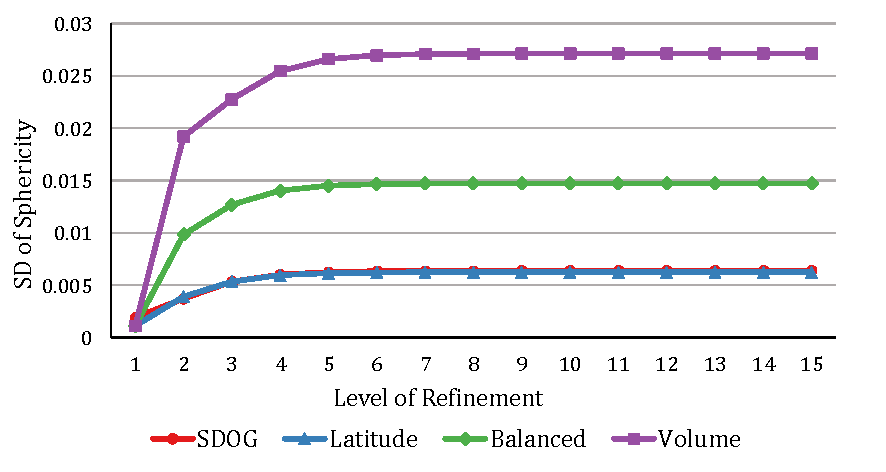
\includegraphics[width=0.8\textwidth]{sd-sph.pdf}
	\caption[Graph of SD of sphericity for the different grids]{
		Standard deviation of sphericity for the different grids at increasing levels of refinement
	}
	\label{fig:sd-sph}
\end{figure}


As a baseline, we have calculated the value of these measures at each refinement level from one to fifteen for conventional SDOG.
We then repeated this for the three modifications discussed in this chapter: the volume method, the latitude method, and the balanced method.
The results for each grid are displayed in Figures~\ref{fig:vr}, \ref{fig:cv}, \ref{fig:sph}, and \ref{fig:sd-sph} showing the volume ratio, CV of volume, mean sphericity, and SD of sphericity, respectively.
Table~\ref{tab:results} summarizes these charts with the convergence value of each property for the four different grids.
We also give convergence values for the maximum and minimum sphericity---and their difference---for each grid in Table~\ref{tab:results-sph}.
It is important to note that for volume ratio and CV of volume, lower values are better, but for sphericity, a higher value is better.


\begin{table}[htp!]
	\centering
	\caption[Convergence values of measures for the different grids]{
		Convergence value of each measure for the different grids
	}
	\begin{tabular}{@{} c c c c c @{}}
		\toprule
		& SDOG    & Latitude & Balanced & Volume   \\ \midrule
		Volume Ratio     & 8.88    & 7.99     & 4.470    & 2.63     \\
		CV of Volume     & 0.412   & 0.399    & 0.201    & $\approx$0 \\
		Mean Sphericity  & 0.799   & 0.797    & 0.786    & 0.768    \\
		SD of Sphericity & 0.00639 & 0.00626  & 0.0147   & 0.0271   \\ \bottomrule
	\end{tabular}
	\label{tab:results}
\end{table}


\begin{table}[htp!]
	\centering
	\caption[Convergence values of max and min sphericity for the different grids]{
		Convergence value of max and min sphericity for the different grids
	}
	\begin{tabular}{@{} c c c c c @{}}
		\toprule
		& SDOG   & Latitude & Balanced & Volume \\ \midrule
		Max sphericity & 0.806  & 0.806    & 0.806    & 0.806  \\
		Min sphericity & 0.754  & 0.765    & 0.730    & 0.672  \\
		Difference     & 0.0520 & 0.0406   & 0.0761   & 0.134  \\ \bottomrule
	\end{tabular}
	\label{tab:results-sph}
\end{table}


The latitude method has a better volume ratio than conventional SDOG for all levels of refinement except the first and fourth, and a lower CV of volume for all levels of refinement after the second.
However, the mean sphericity of cells in this method is slightly reduced as compared to conventional SDOG.
The variation in sphericity is nearly identical between these two refinement methods, with the latitude one having a minuscule reduction.


As to be expected, with all NG cells having equal volume, the volume method gives a much larger improvement to both the volume ratio and the CV of volume for all refinement levels but the first.
As the level of refinement gets large, the CV of volume quickly approaches zero since the number of NG cells is much larger than the number of LG and SG cells in the grid.
The cost of this improved volume preservation is a much larger reduction in the sphericity of cells and an increase in the variation of sphericity, which is also to be expected.


By construction, the balanced method has measures in between that of conventional SDOG and the volume method.
The CV of volume, mean sphericity, and SD of sphericity are all near the respective halfway points, whereas the volume ratio still ends up being a significant improvement over conventional SDOG.

\section{Summary}
This chapter presents modifications of conventional SDOG refinement that result in improved volume preservation properties in the resulting grids.
The modifications improve volume preservation as measured by two different metrics at the cost of reducing cell compactness.
Two blending functions---each defined on a single parameter---enable different balances between volume preservation and compactness.
When used for maximum volume preservation, our method results in all non-degenerate cells in the grid having exactly equal volume.

\chapter{Extending 2D DGGS's to Three Dimensions} \label{chap:extension}
While SDOG and its variants proposed in the previous chapter have many desirable properties, it may not be the ideal 3D DGGS in all circumstances.
The varying uses for a DGGS means each application has different needs of the DGGS it employs.
As such, no single DGGG---2D or 3D---is ideal for every use case.
Therefore, there is a need for many different DGGS's, each with unique properties and intended use cases.


Addressing the needs of different applications, researchers have developed a large variety of different 2D DGGS currently available; the creation of new 3D DGGS's should build off these existing methods.
A natural way to do so is with a method to extend a DGGS to 3D, as seen in~\cite{xie2013interactive} and~\cite{sirdeshmukh2019utilizing}.
However, existing extension methods are not generalizable to any possible DGGS and fail to address cell degeneration toward the centre of the grid.
In this chapter, we aim to address these shortcomings.
We present a general method for extending \textit{any} existing DGGS, referred to as the input DGGS, to the third dimension using a semiregular degenerate refinement strategy.
This extension is done with care to allow the efficient and straightforward transference of data between 2D and 3D while preserving---as best as possible---desirable properties of the input DGGS in the 3D one.
Figure~\ref{fig:extension} shows an overview of the method.
This chapter discusses only the creation of grid geometry; mapping and coding are discussed in Chapters~\ref{chap:mapping} and \ref{chap:coding}, respectively.


\begin{figure}[ht!]
	\centering
	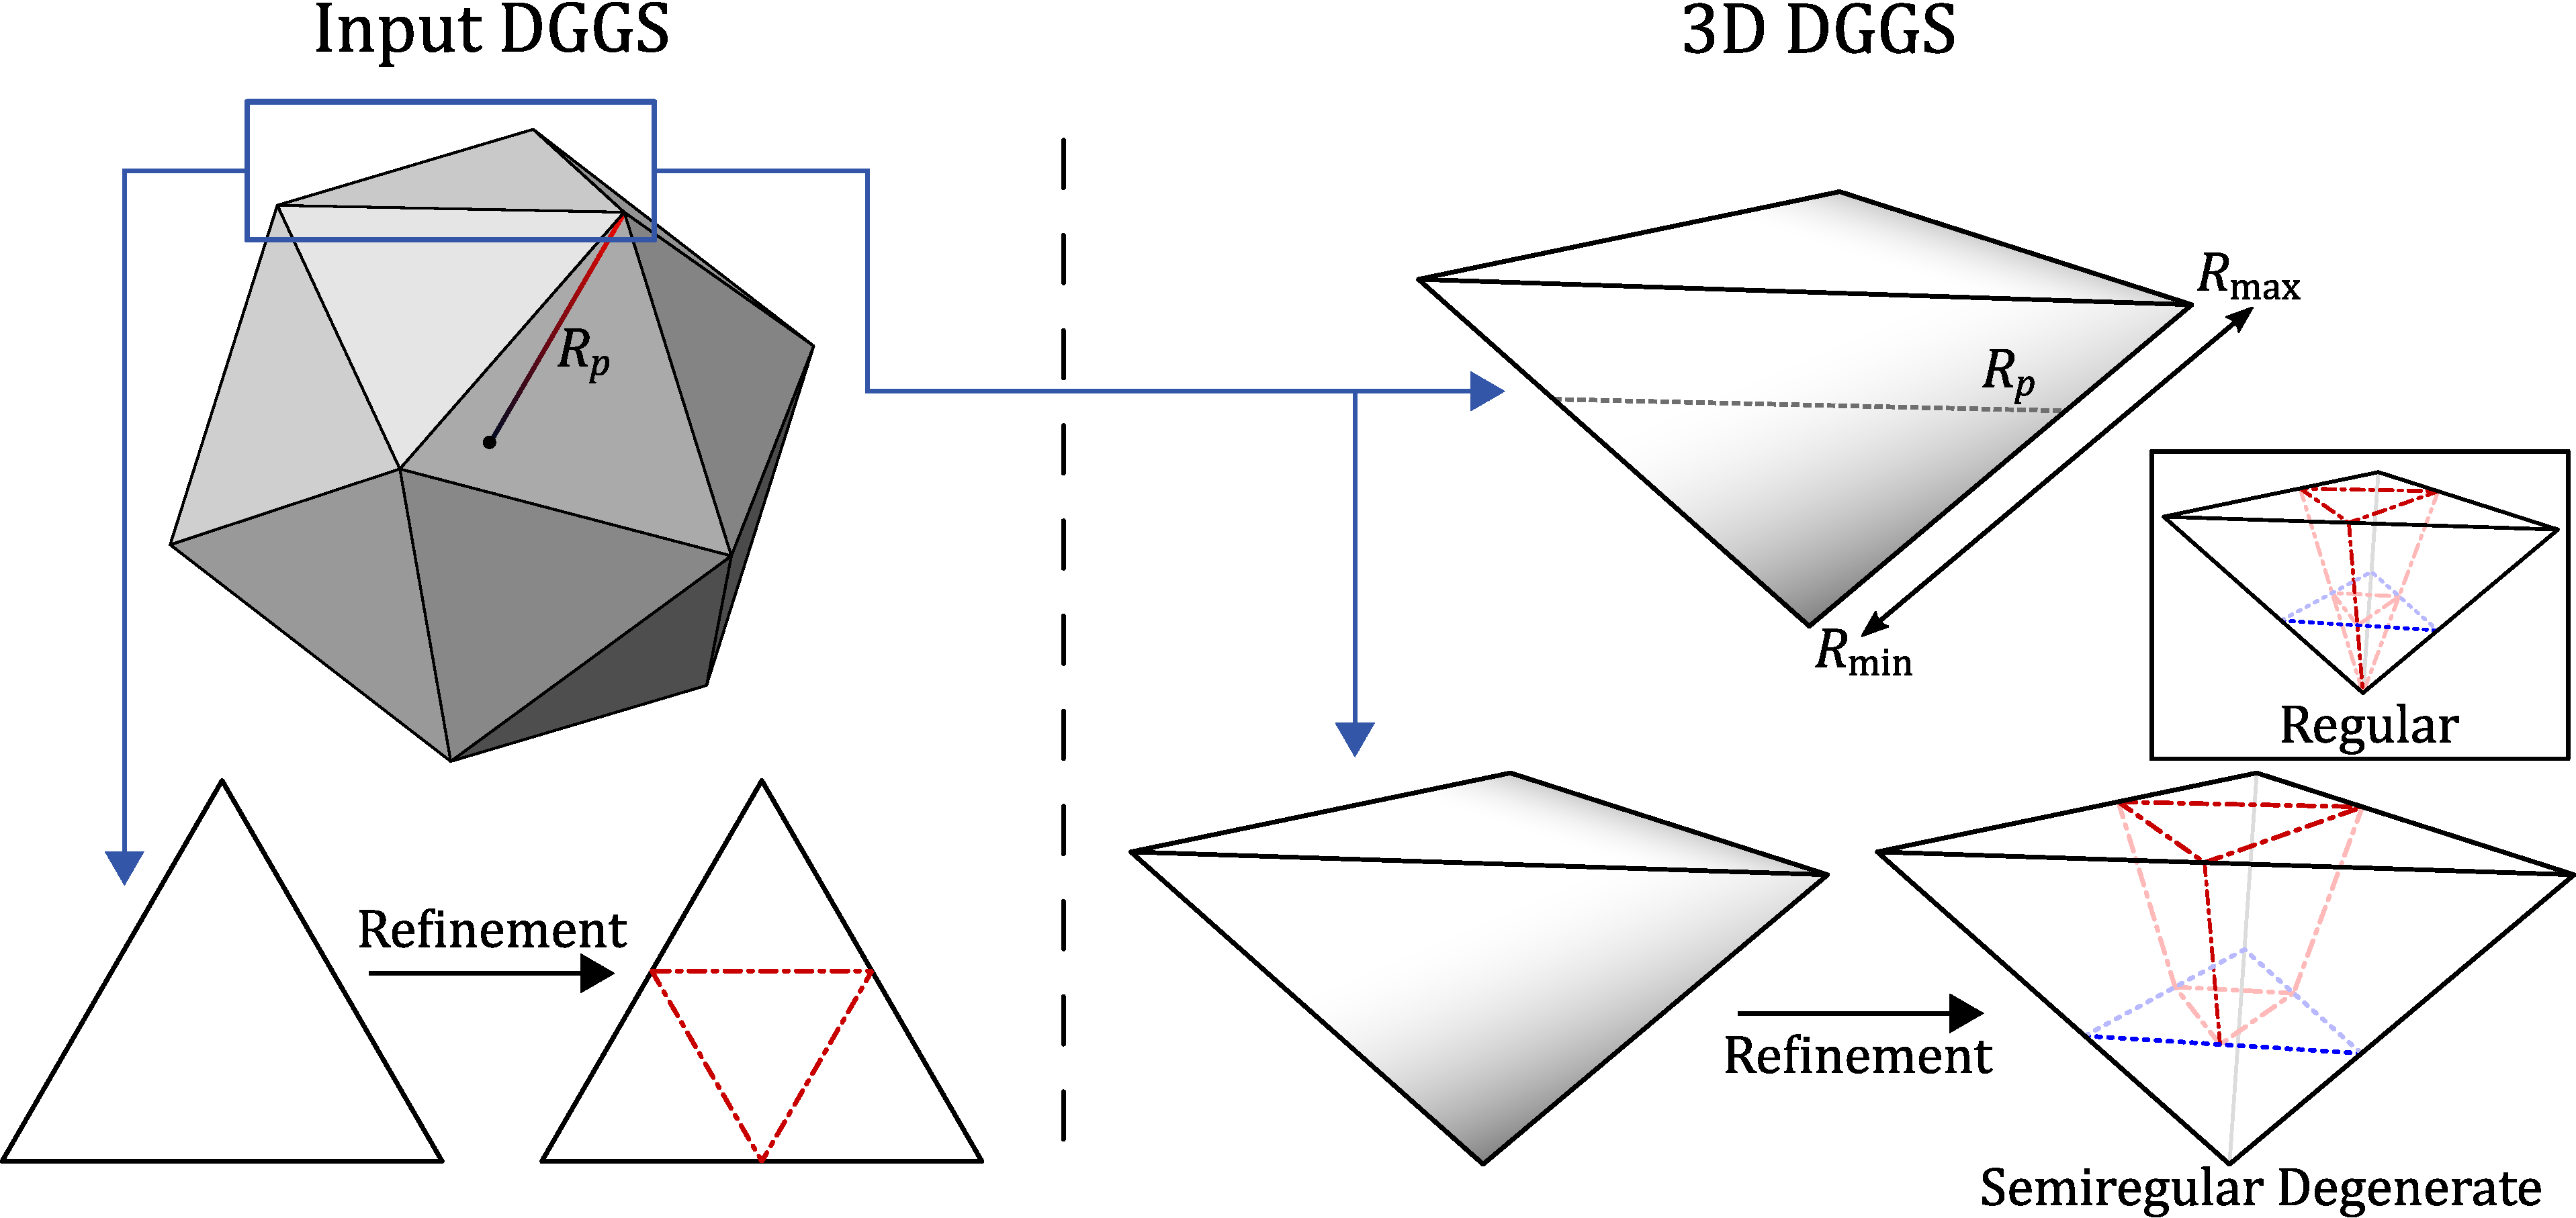
\includegraphics[width=\textwidth]{grid-extension-overview.pdf}
	\caption[Overview of the grid extension method]{
		Overview of how the input DGGS is used to define the geometry of the 3D DGGS.
		The faces of the initial polyhedron of the input DGGS are first extruded to create the prismatoid base cells of the 3D DGGS.
		For refinement, the bases of these prismatoid cells are refined using the same refinement scheme as the input DGGS and combined with a radial refinement.
		A semiregular degenerate refinement is suggested; however, regular refinement is also possible
	}
	\label{fig:extension}
\end{figure}


The content of this chapter is taken from the article "General Method for Extending Discrete Global Grid Systems to Three Dimensions," authored by Benjamin Ulmer, John Hall, and Faramarz Samavati, which appeared in the journal \textit{ISPRS International Journal of Geo-Information} in a special issue on Global Grid Systems~\cite{ulmer2020general}.
Slight modifications have been made to maintain consistent terminology with the rest of the thesis.


\section{Prismatoid Grid Generation and Refinement} \label{chap:5:grid}
Using the input DGGS as a specification, our goal is to define the key elements of the corresponding 3D DGGS logically and consistently.
Below, we discuss the approach for generating the initial discretization and define regular and semiregular degenerate refinement methods. 


\subsection{Initial 3D Discretization} \label{chap:5:discretization}
Let $R_\mathrm{min}$ and $R_\mathrm{max}$ be the minimum and maximum radii that are to be supported by the 3D DGGS, respectively.
The initial 3D discretization, then, is generated from two copies of the initial discretization of the input DGGS at these radii with their edges connected.
For an input DGGS defined directly on the sphere, the radius is well defined.
For a polyhedron-based DGGS, we need to define this radius.
Since the polyhedron is serving as an approximation of the sphere, we define the radius of a polyhedron to be the radius of its circumscribed sphere.
Thus, all points on a polyhedron have the same `radius' (Figure~\ref{fig:layers}).


\begin{figure}[ht!]
	\centering
	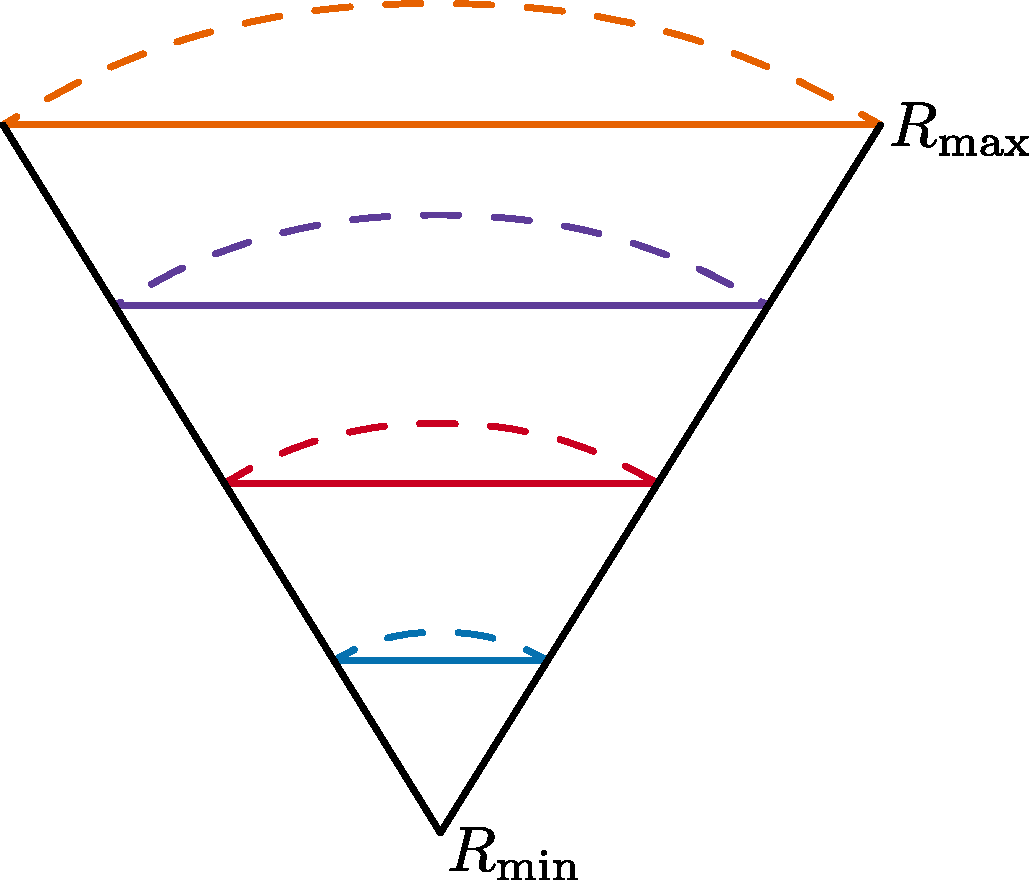
\includegraphics[width=0.5\columnwidth]{layers.pdf}
	\caption[How the radius of a polyhedron is defined]{
		We define the radius of a polyhedron as the radius of its circumscribing sphere.
		In this figure, all points on a solid line of a given colour have the same radius as they all have the same circumscribing sphere (i.e. lie on the same polyhedron).
		The corresponding spheres are shown in the same colours but with a dashed line
	}
	\label{fig:layers}
\end{figure}


If the minimum radius of the 3D DGGS is zero, the base cells are pyramids; otherwise, they are frusta.
In both cases, the cells belong to a parent class of polyhedra known as prismatoids.
For the remainder of this thesis, we assume that $R_\mathrm{min} = 0$; however, other values can be supported by truncating the resulting grid below the desired minimum.
With this discretization, each cell represents the full radial domain of the grid---subsequent refinements will address this issue.


\subsection{Regular Prismatoid Refinement} \label{chap:5:regular}
With an initial 3D discretization for the space of the grid system, we now need a method for refining cells to create more fine discretizations.
We also want to ensure that the 3D DGGS will make use of the same refinement scheme used by the input DGGS, referred to as the surface refinement.
For simplicity, we initially assume the surface refinement factor is 1:4; a generalization to other refinement factors is given later in Chapter~\ref{chap:5:factors}.


\begin{figure}[ht!]
	\centering
	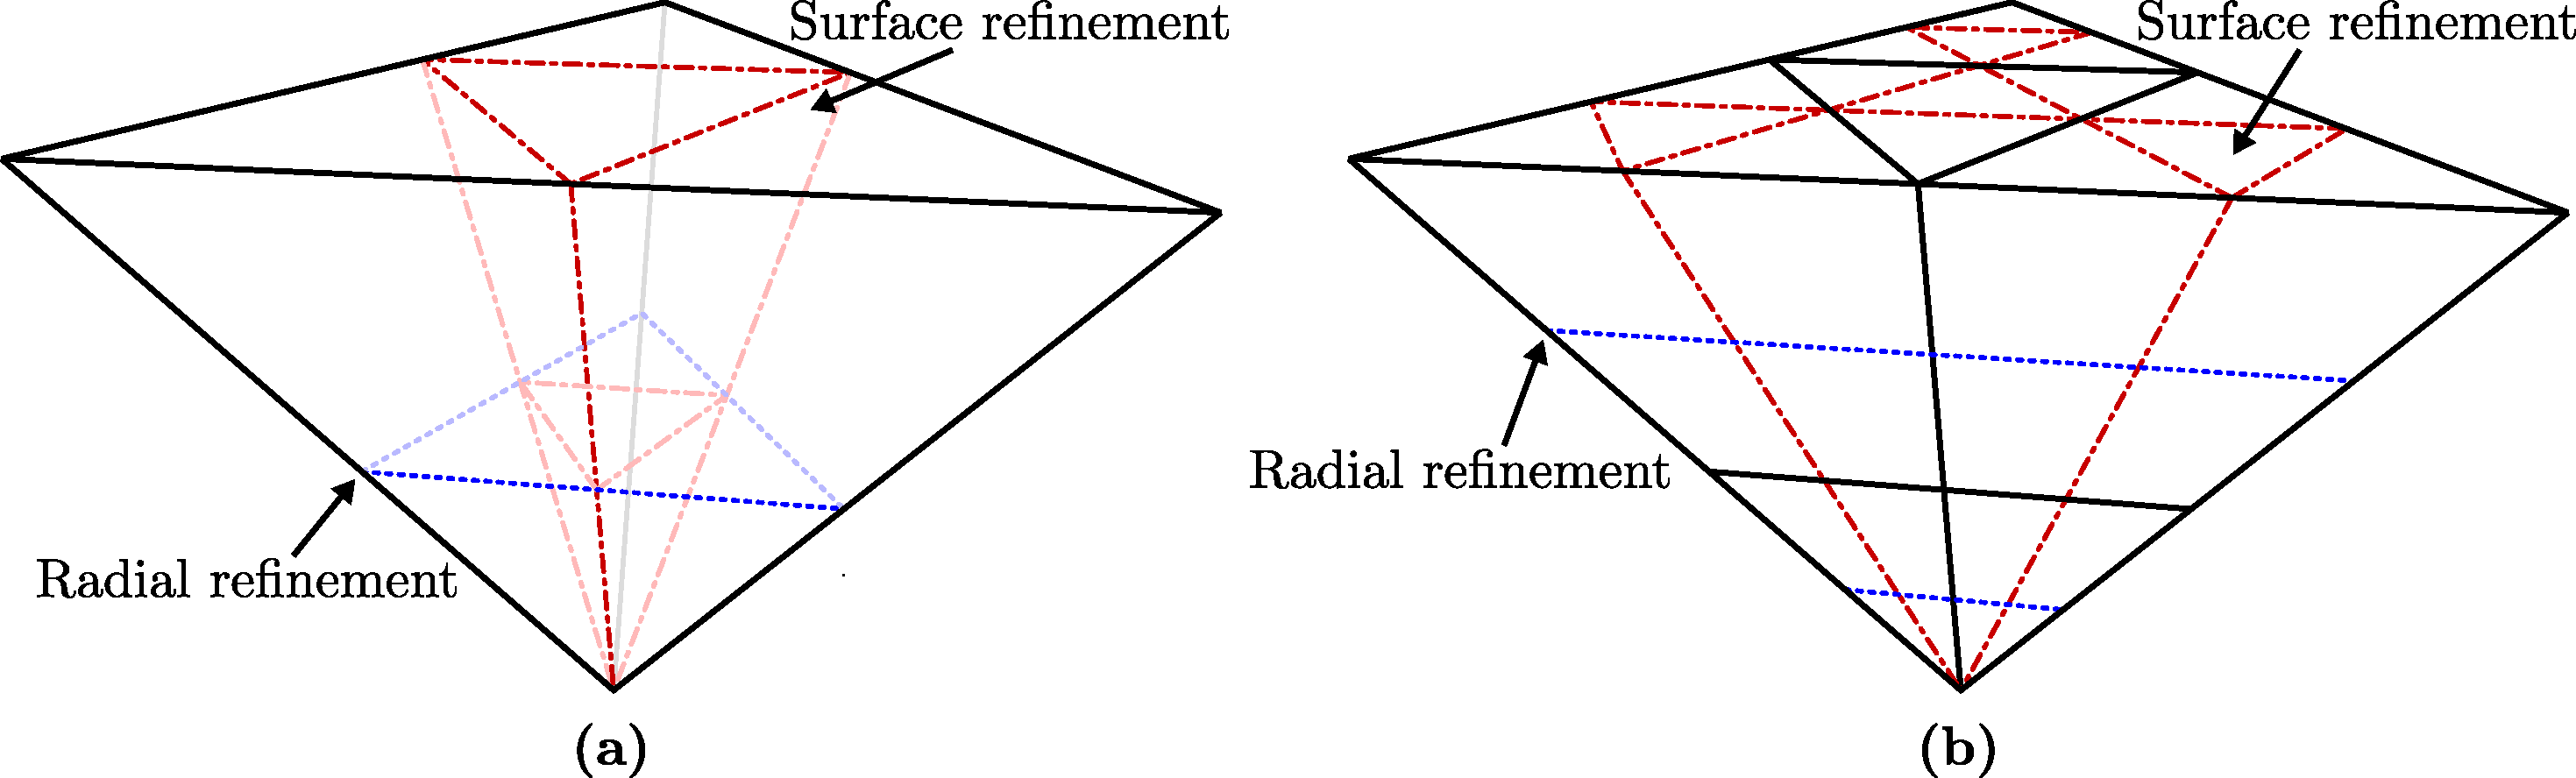
\includegraphics[width=\columnwidth]{reg-refinement.pdf}
	\caption[Regular prismatoid refinement]{
		Regular prismatoid refinement as applied to a single pyramid cell (a) once and (b) twice
	}
	\label{fig:regular}
\end{figure}


Figure~\ref{fig:regular} demonstrates the regular method for refining prismatoid cells.
The bases of the cells are refined using the surface refinement and the resulting edges extruded to meet.
At the same time, a radial split is placed at the midpoint of the two bases.
This refinement results in an inner and outer layer of cells, each containing the same number of cells as one another.
The outer layer is always composed of frustum cells, whereas the inner layer has the same shape as the cells that were being refined.
Defining the refinement in terms of layers of cells as opposed to individual cells allows for native accommodation of non-congruent surface refinements.


\subsection{Semiregular Degenerate Prismatoid Refinement} \label{chap:5:semireg}
While the regular prismatoid refinement proposed above is simple, it has the same issues near the central singularity as other Earth-centric 3D DGGS's.
To address this issue, we define a semiregular degenerate refinement for the prismatoid cells.
Aiding in this, we classify the layers of the grid as either central or normal.
We use $r_\mathrm{min}$ and $r_\mathrm{max}$ to refer to the minimum and maximum radius of a layer, respectively.
As with the polyhedra used for the initial discretization, these radii are equal to the radii of the circumscribing spheres.
Central layers are those that border the central singularity of the grid ($r_\mathrm{min} = 0$), and all other layers are considered normal.
By definition, at any resolution of the 3D DGGS, there is only one central layer.
Furthermore, the initial discretization is entirely composed of this central layer.
We continue our assumption of a 1:4 surface refinement factor from before.


\begin{figure}[ht!]
	\centering
	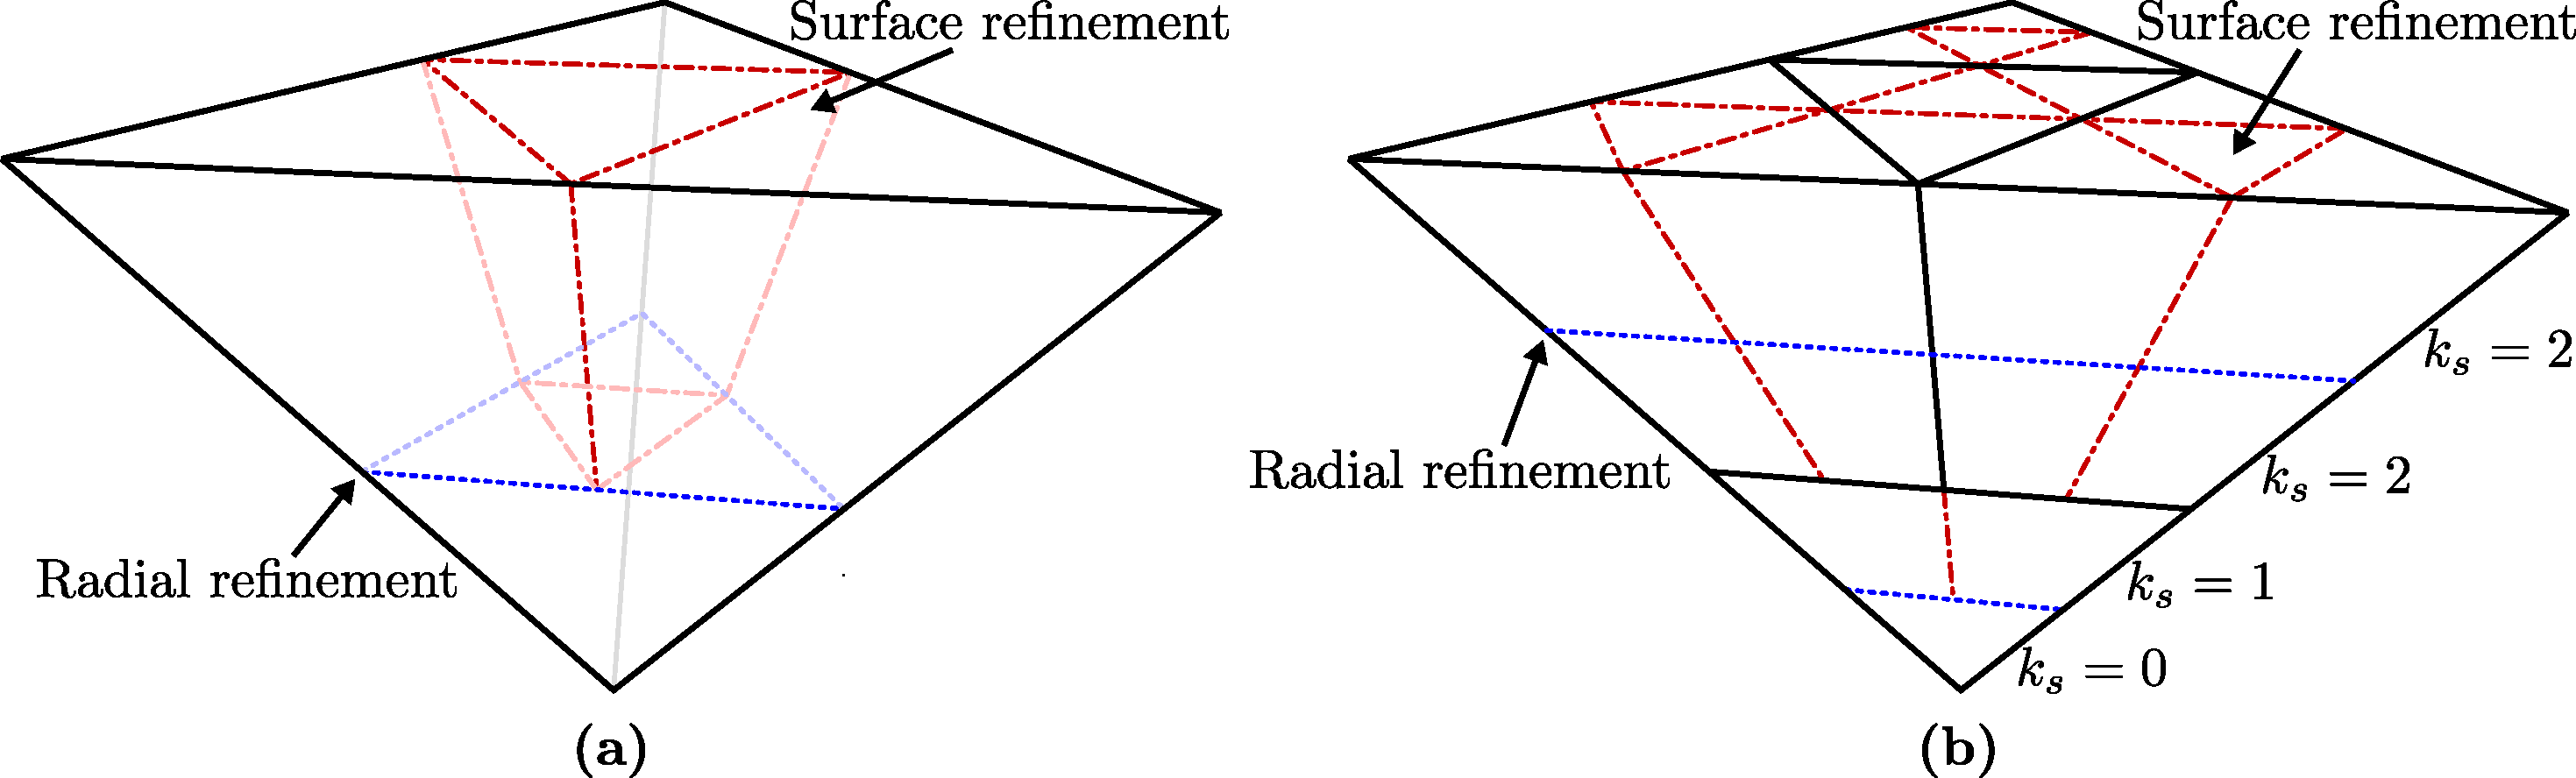
\includegraphics[width=\columnwidth]{semireg-refinement.pdf}
	\caption[Semiregular degenerate prismatoid refinement]{
		Semiregular degenerate prismatoid refinement as applied to a single pyramid cell (a) once and (b) twice.
		In (b), the number of times the surface refinement has been applied ($k_s$) is shown for each layer; see how the radial refinements of central layers separate regions of the grid with different values of $k_s$}
	\label{fig:semiregular}
\end{figure}


Just as with regular refinement, the bases of the pyramid cells are refined using the surface scheme with a radial split made in the middle of the layer.
However, to make this refinement semiregular degenerate, the new edges do not extend beyond the radial split in the direction toward the centre (Figure \ref{fig:semiregular}).
This refinement results in two new layers: an inner central layer, which is similar to the initial central layer, and an outer normal layer.
As demonstrated in Figure~\ref{fig:semiregular}b, the resolution---or refinement level---a layer appears in at the 3D grid does not necessarily correspond to how many times the surface refinement scheme has been applied.
We define the number of applications of the surface refinement to a given layer as the surface resolution, given by $k_s$.
Thus, if we say the initial discretization has $k_s = 0$, after one level of refinement the inner central layer also has $k_s = 0$, whereas the normal layer has $k_s = 1$.
We require this surface resolution in Chapter~\ref{chap:coding} for grid encoding, decoding, and various indexing queries. As will be seen, however, it can be computed and does not need to be explicitly stored.


\begin{figure}[ht!]
	\centering
	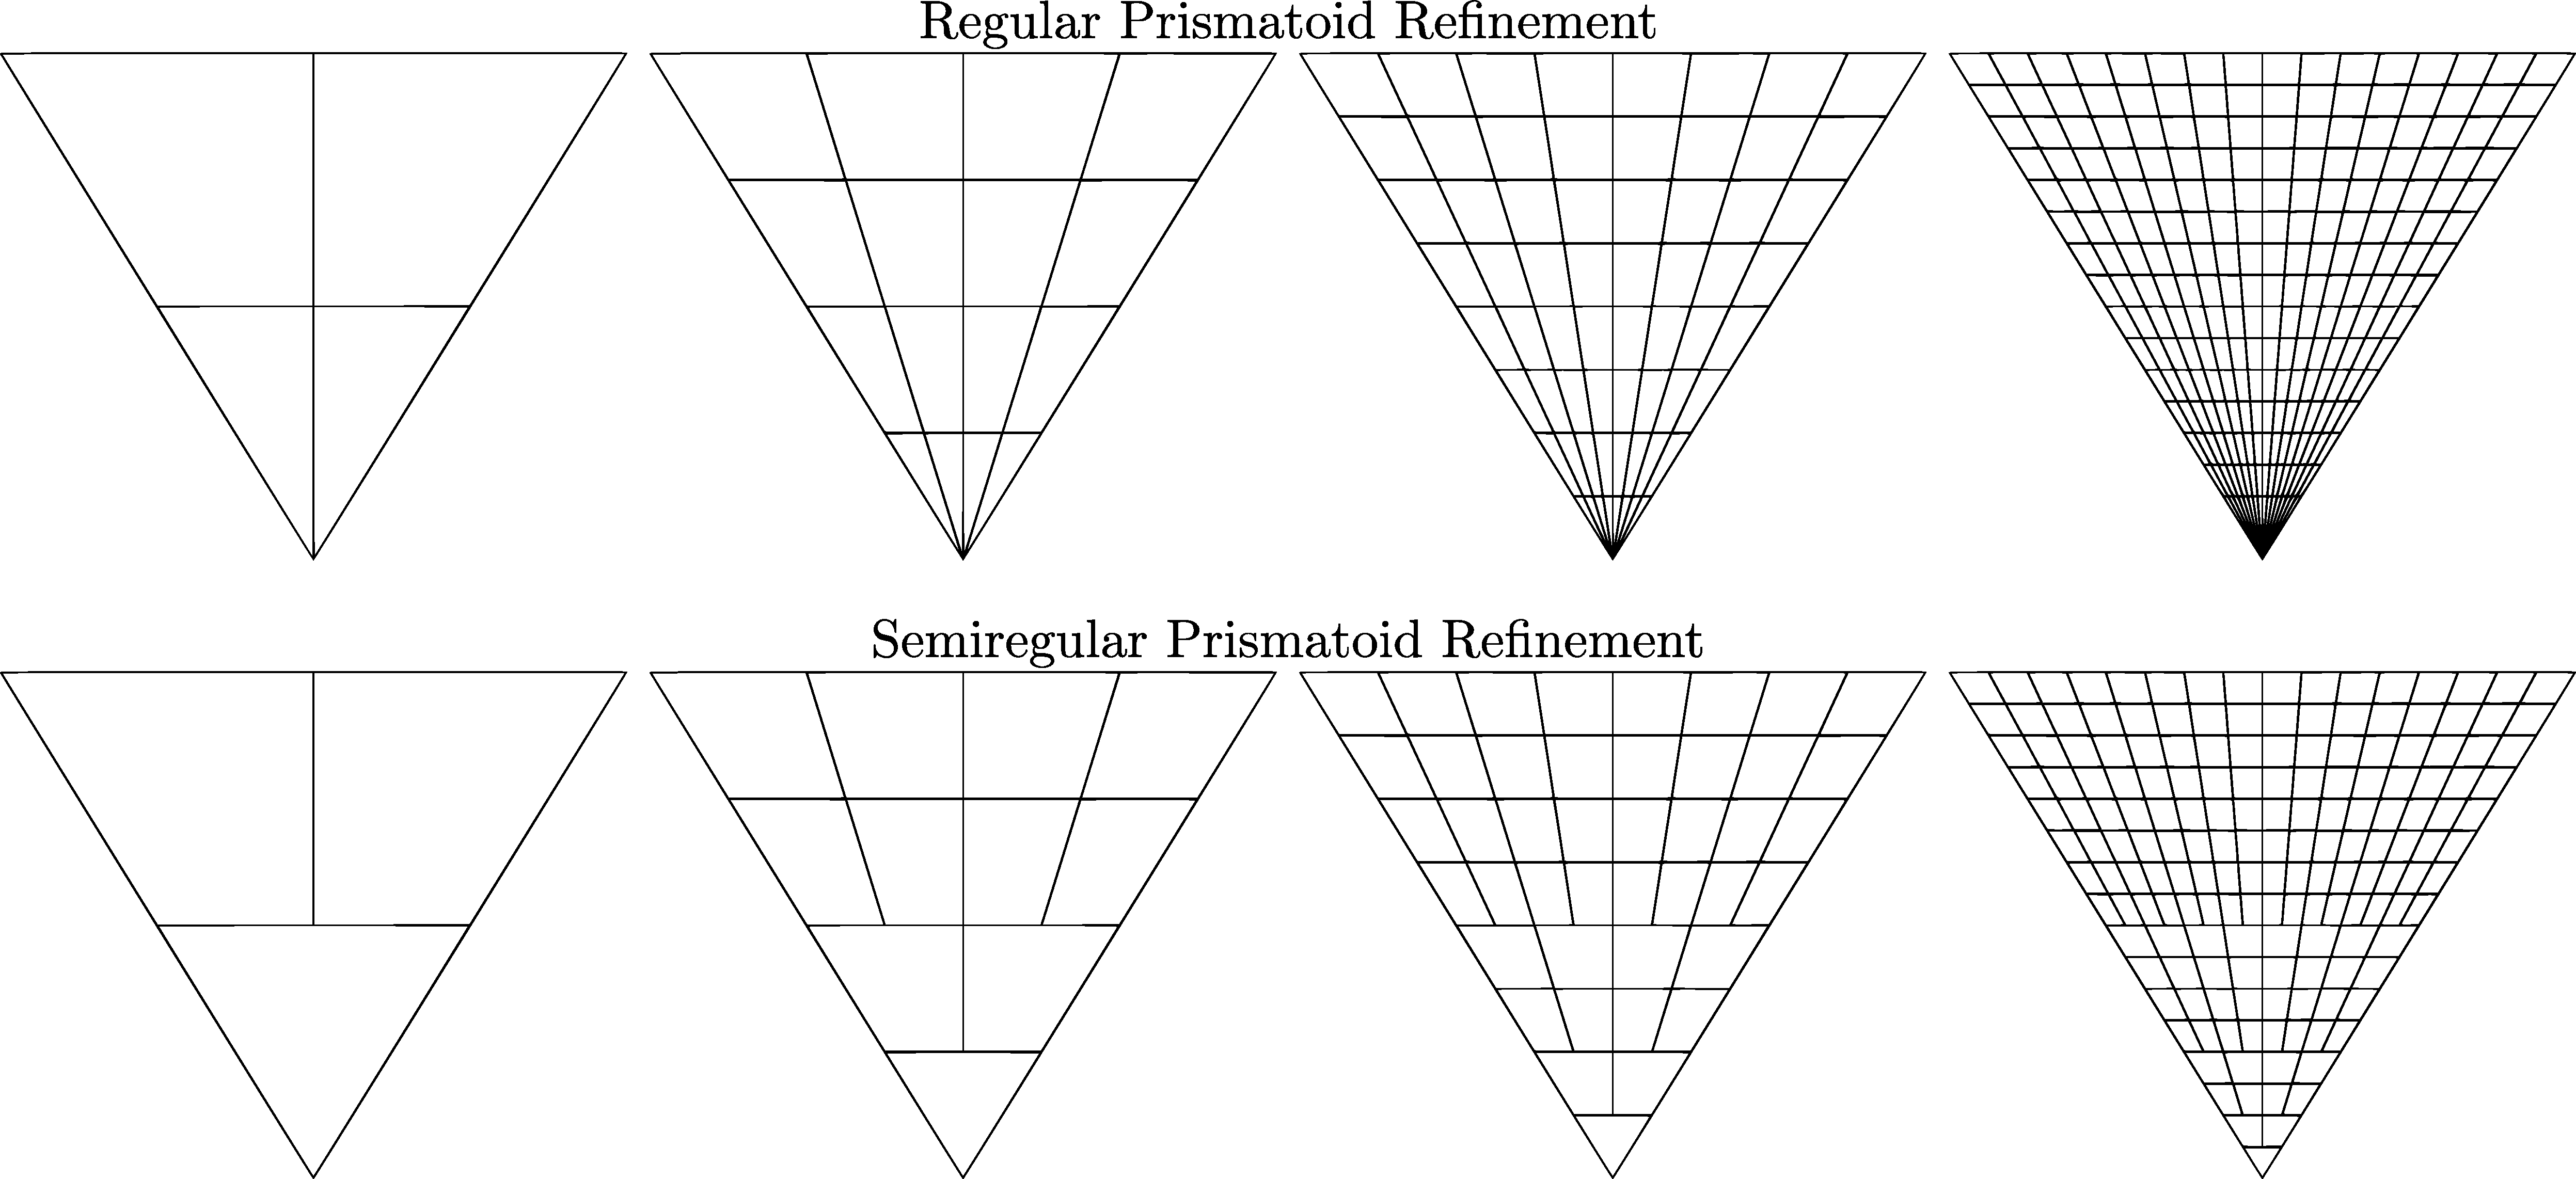
\includegraphics[width=\textwidth]{reg-vs-semireg.pdf}
	\caption[Comparison of regular and semiregular degenerate prismatoid refinement]{
		Three levels of successive applications of regular (top) and semiregular degenerate (bottom) prismatoid refinement.
		Only the side of a single pyramid starting cell is shown to highlight the behaviour of the two schemes at different radii.
		Note how cells degenerate towards the centre with regular refinement, whereas this issue is not present in the semiregular degenerate scheme
	}
	\label{fig:reg-vs-semireg}
\end{figure}


As with other semiregular degenerate refinements, normal layers in this scheme are refined using the regular method.
This regular refinement results in two normal layers, both of which have $k_s$ equal to one greater than that of the starting layer.
Figure~\ref{fig:reg-vs-semireg} compares three successive applications of regular and semiregular degenerate prismatoid refinement to a single pyramid cell.


\subsection{Other Surface Refinement Factors} \label{chap:5:factors}
While it is possible to use the above refinement methods for surface refinement factors other than 1:4, doing so results in a potentially significant issue that should be addressed.
First, we introduce the idea of a one-dimensional (1D) refinement factor, which we find by taking the square root of the surface (2D) one.
For example, the 1D refinement factor of a 1:4 surface refinement scheme (Figures~\ref{fig:regular} and \ref{fig:semiregular}) is 1:2.
While the surface refinement scheme need not be uniform across the two dimensions, the 1D refinement factor gives an idea of the \textit{average} refinement expected along each dimension.


To create uniform cells, it is clear that the refinement factor along the radial dimension for regular prismatoid refinement should be equal to the 1D refinement factor.
If this is not the case, then the width of cells relative to their depth is not constant between refinement levels, since one dimension is refined more quickly.
For a surface refinement factor of 1:4, the single radial split used matches this exactly (one split creates two new layers).
For other surface refinement factors, the 1D and radial refinement factors are not necessarily equal, and cell shape will degenerate---becoming either increasingly narrow or wide---as refinement continues.


To address this issue, we modify the number of radial splits performed such that the number of layers produced is equal to the 1D refinement factor.
For surface refinement factors that are perfect squares (e.g.
1:4, 1:9) this is trivial, as the 1D refinement factor is an integer; the corresponding radial refinement factor is achieved by creating a number of layers equal to the 1D factor.
For other surface refinement factors, though, this becomes more difficult.
The 1D refinement factor is no longer an integer, and since we can only perform a whole number of radial splits, the 1D and radial refinement factors cannot be exactly equal.
Therefore, we propose performing a different number of radial splits at different levels of refinement to make the \textit{average} radial refinement factor equal to the 1D one.


There are a few different methods that can be used to determine the number of radial splits to perform at a given refinement level.
The most straightforward method is to alternate between producing one layer (i.e.
no splits) and producing a number of layers equal to the surface refinement factor.
When the surface refinement factor is not a prime number, a better method is to alternate between the two members of a factor pair, such as two and three for a 1:6 surface factor.
In general, the product of the number of layers at each level of refinement should be equal (or as close as possible) to the 1D refinement factor to the power of the number of refinement levels.
Formally,
%
\begin{equation*}
\prod_{i = 1}^{k} \ell_{i} = f^{k},
\end{equation*}
%
where $\ell_{i}$ is the number of layers produced at refinement level $i$, $k$ is the level of refinement, and $f$ is the 1D refinement factor.
We use this equation iteratively to find the best number of layers for successive levels of refinement with prime surface refinement factors.
Table~\ref{tab:layers} lists our proposed layering sequences for surface refinement factors from 1:2 up to 1:9.


\begin{table}[ht!]
	\centering
	\caption[Layering sequences for different surface refinement factors]{
		Our proposed layering sequences for different surface refinement factors.
		Each number in the sequence is how many layers \textit{normal} layers should split into at the corresponding level of refinement.
		An overline indicates that the sequence repeats indefinitely.
		For semiregular prismatoid refinement, since the initial discretization has no normal layers, these sequences are used starting with the \textit{second} level of refinement
	}
	\begin{tabular}{@{} c l @{}}
		\toprule
		Surface Refinement Factor & Layering Sequence         \\ \midrule
		1:2                  & $\overline{2,1}$               \\
		1:3                  & $\overline{3,1}$               \\
		1:4                  & $\overline{2,2}$               \\
		1:5                  & $2,3,2,2,2,3,2,2,2,3,2,2,3...$ \\
		1:6                  & $\overline{3,2}$               \\
		1:7                  & $3,2,3,3,2,3,3,2,3,3,3,2,3...$ \\
		1:8                  & $\overline{4,2}$               \\
		1:9                  & $\overline{3,3}$               \\ \bottomrule
	\end{tabular}
	\label{tab:layers}
\end{table}


\begin{figure}[ht!]
	\centering
	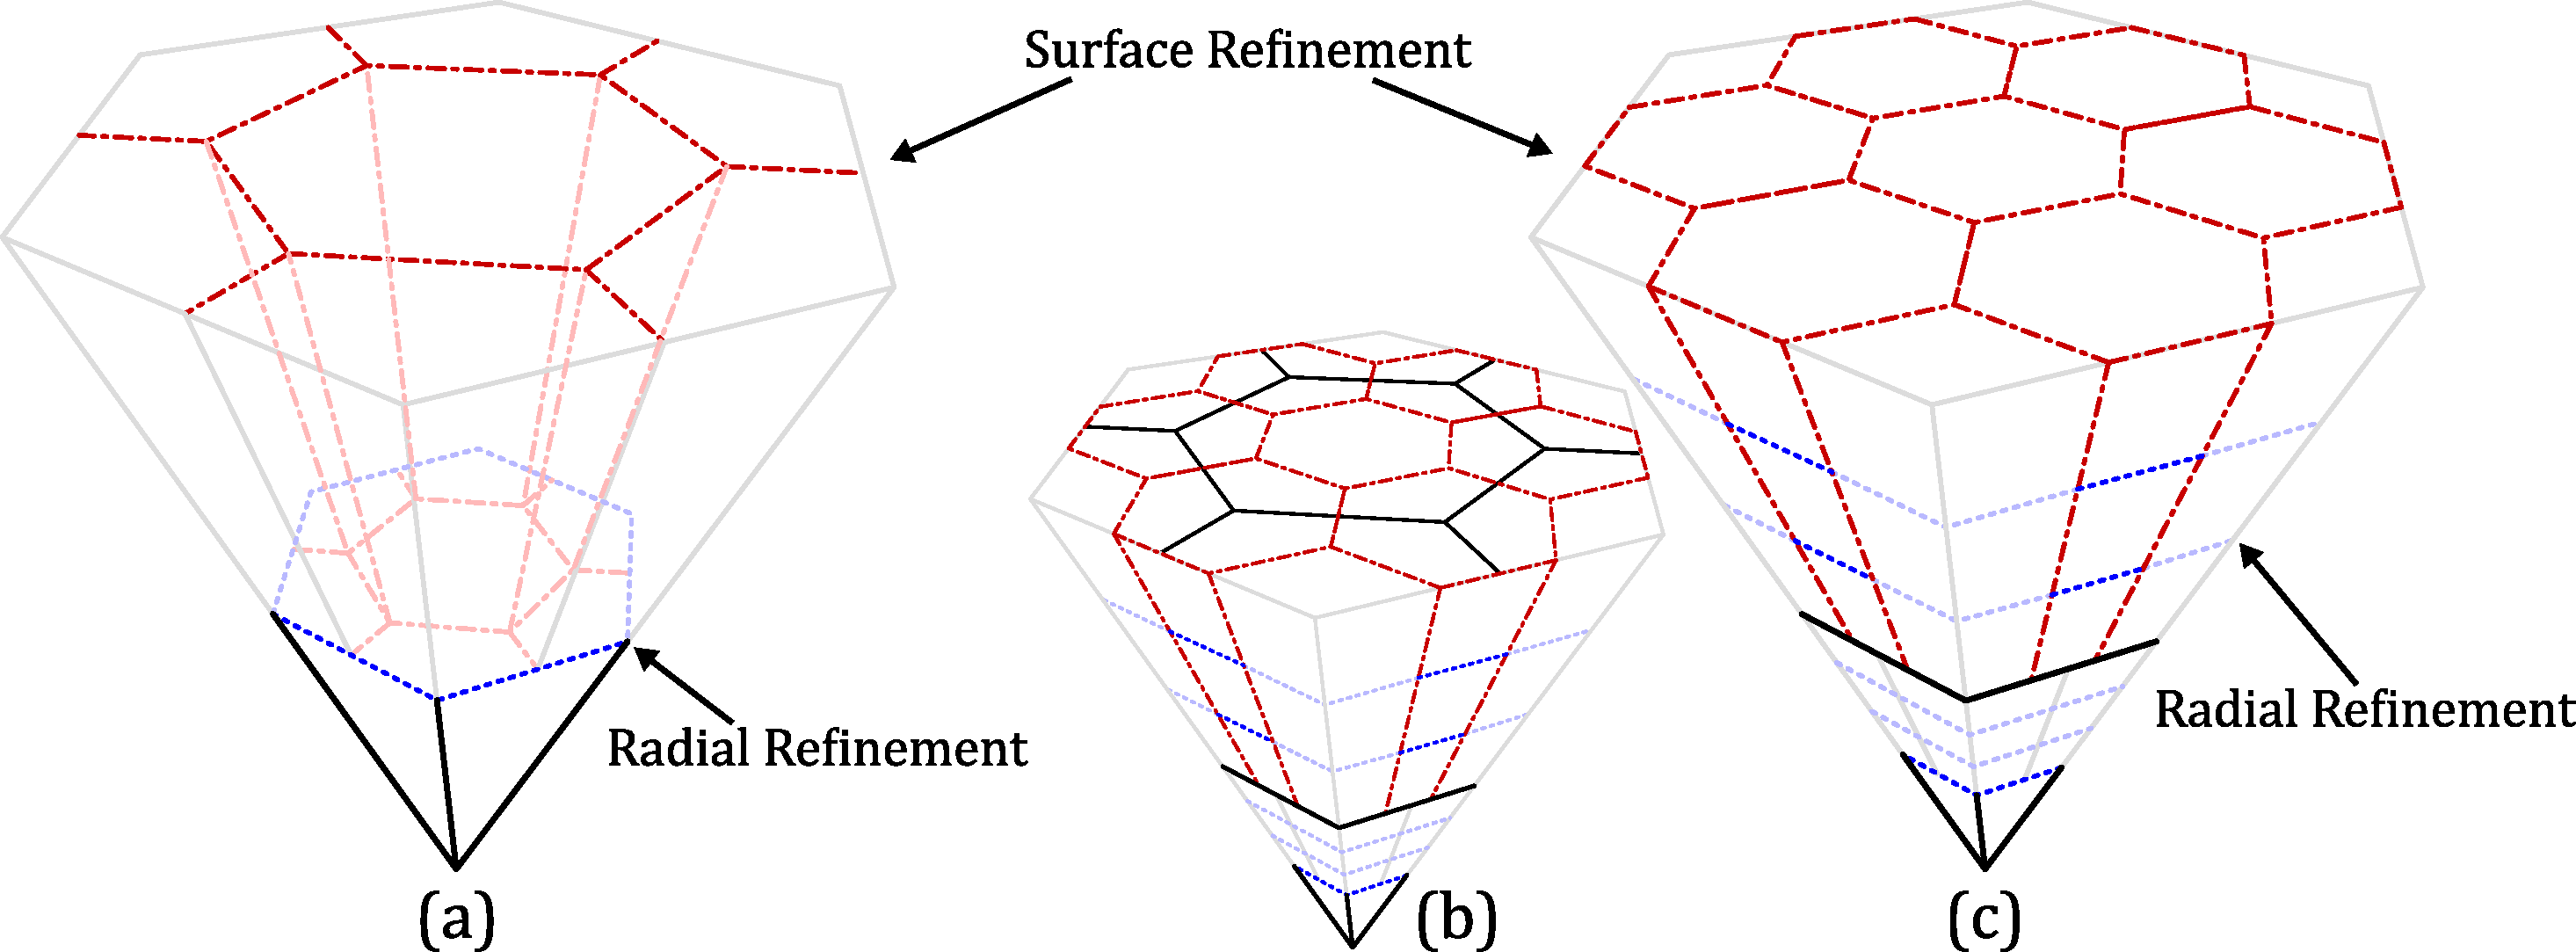
\includegraphics[width=\textwidth]{semireg-hexagons.pdf}
	\caption[Semiregular prismatoid refinement for hexagons]{
		Semiregular prismatoid refinement applied to a hexagonal base cell using a 1:3 surface refinement scheme (a) once and (c) twice; (b) is the same image as (c), but with the surface cells of the previous refinement level shown for reference.
		Note that in the second level of refinement, normal layers have two radial refinements as opposed to one
	}
	\label{fig:hexagons}
\end{figure}


Figure~\ref{fig:hexagons} showcases an example of semiregular prismatoid refinement with a 1:3 hexagonal surface refinement.
The first level of refinement is identical to the cases for a 1:4 surface refinement factor since no normal layers have been refined.
In the second level, however, two radial splits are performed in the normal layers as opposed to one.
In the next level of refinement (not shown), normal layers would not have any radial refinements per the proposed sequence in Table~\ref{tab:layers}.


\section{Cell Aspect Ratio} \label{chap:5:ar}
The surface and radial dimensions of Earth are inherently very different, and because of this, it is often desirable for these two dimensions to be at different resolutions in a 3D DGGS.
For our 3D DGGS's, achieving this entails changing the width of cells in the grid (surface resolution) relative to their depth (radial resolution).
We refer to the ratio between a cell's width and depth as the \textit{aspect ratio} of the cell.
While the refinement methods described thus far produce cells with a similar aspect ratio---both between cells in the same and different resolutions---there is no direct mechanism for controlling what this aspect ratio will be.
To address this issue, we introduce two modifications that can be made to prismatoid refinement to decrease and increase this aspect ratio.


In order to decrease the aspect ratio of cells in the grid, we must increase the number of applications of the surface refinement relative to the number of radial splits.
Since further applications of the prismatoid refinement will maintain the expected cell aspect ratio---a result of the surface and expected radial refinement factors being equal---this only needs to be done the first time a layer would have the bases of its cells refined with the surface scheme.
Thus, for semiregular prismatoid refinement, this is done while refining the outer normal layer that results from refining central layers.
%In the case where only regular prismatoid refinement is used, this is then only done during the first level of refinement.


Likewise, to increase the aspect ratio of cells, we need to decrease the number of times the surface refinement scheme is applied relative to the number of radial splits.
We accomplish this by \textit{not} applying the surface refinement to a layer the first time it would usually be done, and if needed applying additional radial splits at the same time.
These modifications would be done at the same time as the method for decreasing the aspect ratio for the same reasons.


Therefore, given some target cell aspect ratio $a$, we must determine which of the above methods to use.
To do this, we must first quantify the width and depth of a cell.
More specifically, we need to define the average width and depth of cells in a layer, since refinement is performed by layer and not by cell.
Depth comes trivially from the radial extent of the layer ($r_\mathrm{max} - r_\mathrm{min}$).
There are many potential ways to measure the width of a cell; for our purposes, we chose to use the square root of its area.
This choice ensures the framework will produce consistent results for input polyhedra with the same number of faces, irrespective of the shape(s) of said faces.


For the region of outer normal layer(s) generated by refining central layers, the average depth of cells is the total depth of the region divided by the number of layers in the region (assuming no applications of the surface refinement scheme).
Let $\upsilon$ be the percentage of $r_\mathrm{max}$ occupied by this region and $x$ be the number of extra radial splits, then the average depth of cells is
%
\begin{equation*}
\frac{\upsilon r_\mathrm{max}}{x+1}.
\end{equation*}
%
Likewise, the average cell width in this region is the surface area of the sphere divided by the number of cells (assuming no extra radial splits).
Let $n$ be the number of faces on the input polyhedron and $w$ be the number of times the surface refinement is applied, then the number of cells is $n f^{2w}$, and the average cell width is
%
\begin{equation*}
\sqrt{ \frac{ 4 \pi r_\mathrm{max}^2 }{ n f^{2 w} } } = \frac{2 r_\mathrm{max}}{f^w} \sqrt\frac{\pi}{n}.
\end{equation*}
%
We now equate these using the desired aspect ratio to solve for $x$ and $w$, giving
%
\begin{equation*}
a \frac{\upsilon}{x+1} = \frac{2}{f^w} \sqrt\frac{\pi}{n}.
\end{equation*}
%
As to not violate our prior assumptions, when solving for one variable the other is set to zero; this ensures only one of the two strategies for modifying the aspect ratio is employed.
Setting $w = 0$ we get
%
\begin{equation}
x = \frac{a \upsilon}{2} \sqrt{\frac{n}{\pi}} - 1,
\label{eq:extraSplits}
\end{equation}
%
and setting $x = 0$ we get
%
\begin{equation}
w = \log_{f} \left( \frac{2}{a \upsilon} \sqrt{ \frac{\pi}{n}} \right).
\label{eq:num2D}
\end{equation}


\begin{figure*}[ht!]
	\centering
	\begin{subfigure}[]{0.25\textwidth}
		\centering
		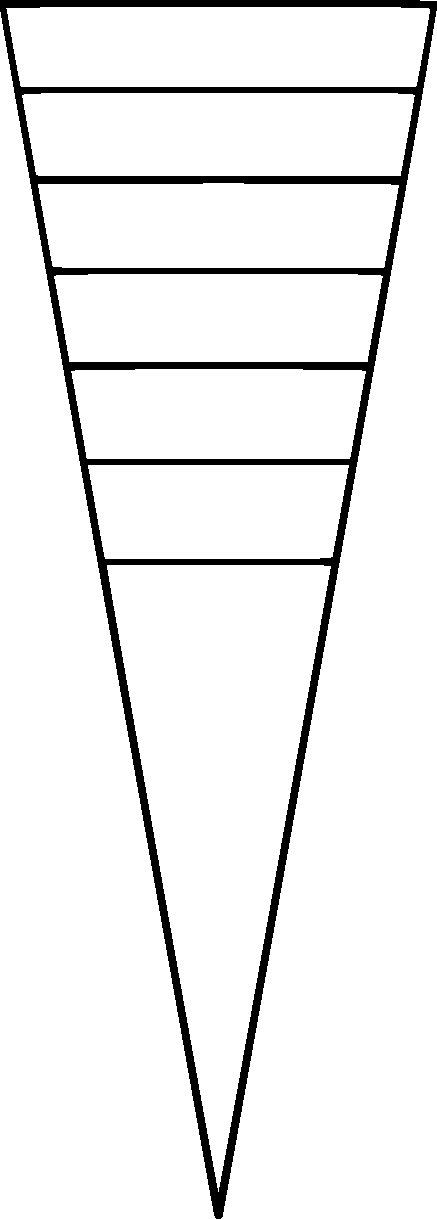
\includegraphics[width=0.5\columnwidth]{5-ers.pdf}
		\caption{}
		\label{fig:ers1}
	\end{subfigure}%
	%
	\begin{subfigure}[]{0.25\textwidth}
		\centering
		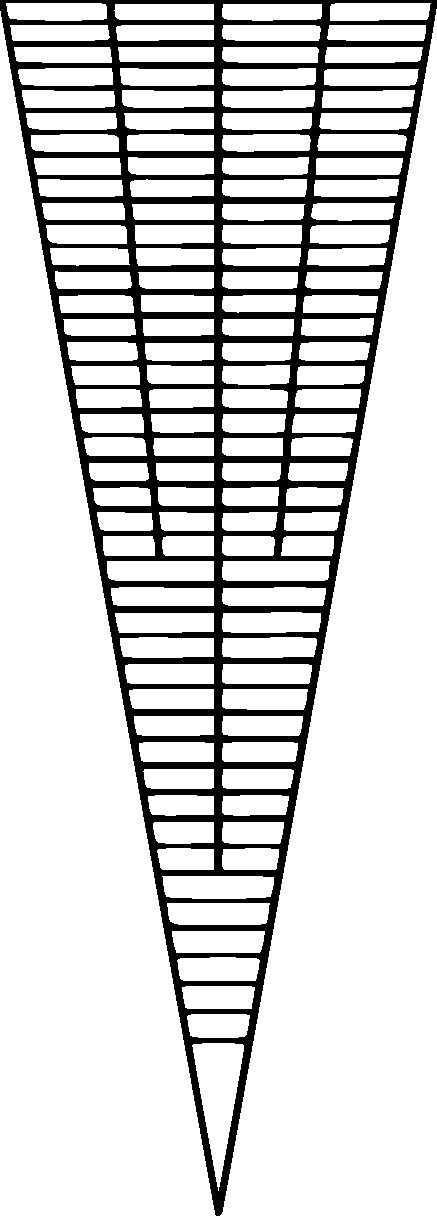
\includegraphics[width=0.5\columnwidth]{5-ers3.pdf}
		\caption{}
		\label{fig:ers3}
	\end{subfigure}%
	%
	\begin{subfigure}[]{0.25\textwidth}
		\centering
		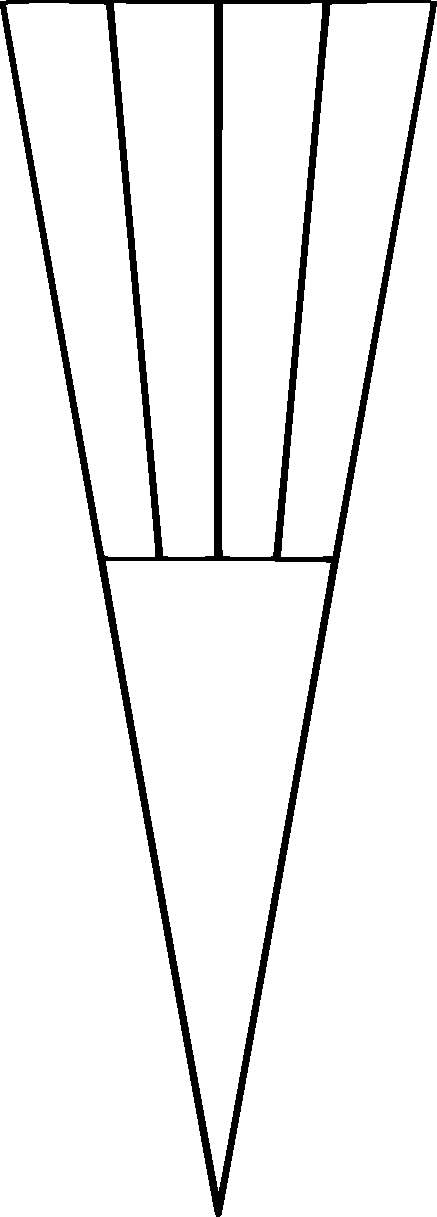
\includegraphics[width=0.5\columnwidth]{2-ess.pdf}
		\caption{}
		\label{fig:ess1}
	\end{subfigure}%
	%
	\begin{subfigure}[]{0.25\textwidth}
		\centering
		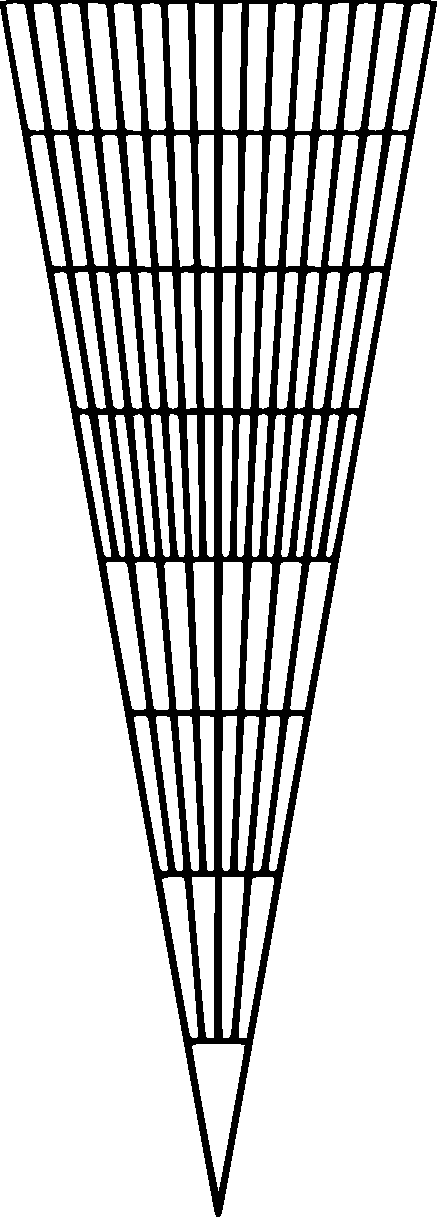
\includegraphics[width=0.5\columnwidth]{2-ess3.pdf}
		\caption{}
		\label{fig:ess3}
	\end{subfigure}
	
	\caption[Prismatoid refinement modified to achieve different cell aspect ratios]{
		A demonstration of how refinement can be modified to affect the aspect ratio of cells.
		All figures show a starting pyramid cell from a grid with 200 cells in its initial discretization.
		Central layer with five extra radial splits ($a = 3$ to get $x = 5$) at (a) one level of refinement and (b) three levels.
		Central layer with two applications of the surface refinement scheme ($a = 1/8$ to get $w = 2$) at (c) one level of refinement and (d) three levels
	}
	\label{fig:extraDPS}
\end{figure*}


The actual values of $x$ and $w$ selected for use is determined by which one is negative.
If $x$ is negative, it is set to zero, and the value of $w$ is used---vice versa for if $w$ is negative.
Since $x$ or $w$ may not be integers, we simply round them to the nearest whole number to get the actual value used during refinement.
The results of refinement with different target aspect ratios are demonstrated in Figure~\ref{fig:extraDPS}.


\section{Summary}
This chapter provides a complete and comprehensive method for extending any 2D DGGS into a 3D DGGS.
The approach is general and properly accommodates any potential DGGS regardless of the initial polyhedron, refinement, or projection employed.
Semiregular degenerate refinement allows unbounded ranges of altitudes without significant degradation in cell shape or size.
Techniques are employed to ensure cells have the desired aspect ratio while maintaining the aspect ratio and relative volume of cells during refinement.
The following chapters explain how to handle mapping and coding with these grids. 

\chapter{Mapping Techniques for SDOG and Prismatoid Grids} \label{chap:mapping}

\subsection{SDOG Indexing} \label{sec:sdog-indexing}
In order to identify and distinguish the cells of a grid, there needs to be a method to assign a unique index to each cell.
A good indexing scheme will allow for efficient data insertion, retrieval, and manipulation via a set of queries.
Examples of some of these queries are: point to cell, which give the index of the cell containing a given point; index inversion, which calculates a cell's location and geometry from the index; neighbourhood queries; and in the case of a hierarchical grid, hierarchy traversal to find parent and children cells.


Due to the fact that SDOG refinement is based on the midpoints of spherical coordinates, an indexing scheme that is efficient for many of the above operations can be easily developed.
At any refinement level, $k$, each cell can be given an integer index in each spherical coordinate ranging from zero to $2^{k} - 1$.
To address the degenerate refinement of certain cells, these integer indices are modified appropriately with divisions by powers of two, which can be done quickly with bit shift operations.
The integer indices can then be linearized by various methods, one good choice being a Z-order curve \cite{morton1966computer} as used in \cite{yu2009sdog}.
A more detailed description of degenerate Z-order indexing for SDOG grids, including algorithms for point to cell and index inversion operations, can be found in \cite{yu2009coding}.


\section{Radial Mappings}
\section{Latitude Mappings for SDOG}

%\section{Mapping Modified SDOG Grids} \label{sec:mapping}
By modifying the splitting surfaces used for subdivision, any SDOG indexing operations that depend on the location of cells in the grid will no longer function properly.
Examples of these operations include point to cell queries, which give the cell that contains a given point, and index inversion, which calculates the location and geometry of a cell from its index.
The obvious solution is to simply redefine these operations on the new geometry, however, this is not necessarily practical as it would have to be done individually for each modified grid.
Additionally, the more complex geometry of the modified grids may make these algorithms more difficult to design and/or more computationally expensive to perform as compared to the ones for conventional SDOG.
A better solution is to find a mapping (and corresponding inverse mapping) between a conventional SDOG grid and the grid resulting from the modified subdivision scheme.
Given this mapping, all indexing operations can be done using the standard algorithms, with inputs and outputs converted between the conventional SDOG grid and the modified one accordingly.


For the stationary subdivision schemes this mapping is straightforward.
Since only the latitudinal splitting surface of SG cells is modified, latitudes in the range $[0, \pm\frac{\pi}{4})$ should be mapped to the range $[0, \pm\alpha_{\phi}^{SG} \frac{\pi}{2})$ and likewise the range $[\pm\frac{\pi}{4}, \pm\frac{\pi}{2}]$ to the range $[\pm\alpha_{\phi}^{SG} \frac{\pi}{2}, \pm\frac{\pi}{2}]$.
This can be done with a simple linear map, and the inverse follows trivially.


For the non-stationary schemes this mapping is more complicated.
We wish to define a function $M \colon (\phi, r) \rightarrow (\phi, r)$ that converts a latitude and radius in a conventional SDOG grid to the corresponding latitude and radius in the modified grid (longitude does not need to be mapped, as it is not changed between the two grids).
The two coordinates act independently of each other, so we can split this function into its two components, $M_{\phi}(\phi)$ and $M_{r}(r)$, and derive each one and its inverse individually.
This is done by parameterizing points inside an NG cell using the function(s) used to calculate its splitting surfaces (Eq.~(\ref{eq:convex}) for conventional SDOG and Eq.~(\ref{eq:radVol}) and (\ref{eq:latVol}) for the modified grid).
NG cells are used for this purpose as all children cells are also NG, and therefore use the same formulations for calculating splitting surfaces.
By finding the boundaries of the coarsest NG cell that contains a given point, these parameterizations can be used to go from one space to the other by finding a relationship between them---in this case $d = \alpha = p$---all of which can be done in constant time.
The final formulations are as follows, with the full derivation found in Appendix \ref{app:map}.
Let $R_m$ be the radius of the grid.
Latitude forward:
%
\begin{equation*}
M_{\phi}(\phi) = \sin^{-1} \left( d u_{v} + \left( 1 - d \right) \ell_{v} \right), \quad \text{where}
\end{equation*}
%
\begin{equation*}
d = \frac{\frac{2\phi}{\pi} - \ell_{c}}{u_{c} - \ell_{c}},
\end{equation*}
%
\begin{equation*}
u_{c} = 1 - \left( \frac{1}{2} \right)^{ \left\lceil \log_{0.5} \left( 1 - \frac{2\phi}{\pi} \right) \right\rceil }, \quad u_{v} = 2 u_{c} - u_{c}^{2}.
\end{equation*}
%
\begin{equation*}
\ell_{c} = 1 - \left( \frac{1}{2} \right)^{ \left\lfloor \log_{0.5} \left( 1 - \frac{2\phi}{\pi} \right) \right\rfloor }, \quad \text{and} \quad \ell_{v} = 2 \ell_{c} - \ell_{c}^{2}.
\end{equation*}
%
%
Radius forward:
%
\begin{equation*}
M_{r}(r) = R_{m} \sqrt[3]{ d u^{3} + \left( 1 - d \right) \ell^{3} }, \quad \text{where}
\end{equation*}
%
\begin{equation*}
d = \frac{\frac{r}{R_{m}} - \ell}{u - \ell},
\end{equation*}
%
\begin{equation*}
u = \left( \frac{1}{2} \right)^{ \left\lfloor \log_{0.5} \left( \frac{r}{R_{m}} \right) \right\rfloor }, \quad \text{and} \quad
\end{equation*}
%
\begin{equation*}
\ell = \left( \frac{1}{2} \right)^{ \left\lceil \log_{0.5} \left( \frac{r}{R_{m}} \right) \right\rceil }.
\end{equation*}
%
%
Latitude inverse:
%
\begin{equation*}
M^{-1}_{\phi}(\phi) = \frac{\pi}{2} \left( d u_{c} + \left( 1 - d \right) \ell_{c} \right), \quad \text{where}
\end{equation*}
%
\begin{equation*}
d = \frac{\sin \phi - \ell_{v}}{u_{v} - \ell_{v}},
\end{equation*}
%
\begin{equation*}
u_{c} = 1 - \left( \frac{1}{2} \right)^{ \left\lceil \log_{0.5} \left( \sqrt{1 - \sin \phi} \right) \right\rceil },
\end{equation*}
%
\begin{equation*}
\ell_{c} = 1 - \left( \frac{1}{2} \right)^{ \left\lfloor \log_{0.5} \left( \sqrt{1 - \sin \phi} \right) \right\rfloor },
\end{equation*}
%
%
and both $u_{v}$ and $\ell_{v}$ follow the same as the forward.
Radius inverse:
%
\begin{equation*}
M^{-1}_{r}(r) = R_m \left( d u + \left( 1 - d \right) \ell \right), \quad \text{where}
\end{equation*}
%
\begin{equation*}
d = \frac{ \left( \frac{r}{R_{m}} \right)^{3} - \ell^{3}}{u^{3} - \ell^{3}}
\end{equation*}
%
and both $u$ and $\ell$ follow the same as the forward.


In the case where a division by zero occurs, (i.e. when $u = \ell$ or $u_{c} = \ell_{c}$), the result of said division is treated as zero.
The latitude mappings assume $\phi \ge 0$, however, from symmetry a negative value of $\phi$ can easily be accommodated by using the absolute value and negating the final result.
This mapping is applicable to the first non-stationary scheme discussed in Section \ref{sec:method-nonStationary}; schemes derived from Eq.~(\ref{eq:beta}) cannot be mapped, as this formulation cannot easily be expressed in terms of a parameter.
In the future, other blending methods may be explored that allow for a similar mapping to be derived.




\section{Summary}
\chapter{Efficient Encoding, Decoding, and Indexing} \label{chap:coding}
The mappings described in the previous chapter are only one part of the process for associating geospatial data to cells of a 3D DGGS.
With geospatial data mapped to the grid system's domain, the set of cells associated with the geometry of the data---and the indices of said cells---must be obtained.
As described earlier, this entire process is known as grid encoding.
Likewise, there needs to be a process to obtain the geometry of a cell (in grid space) from its index, so that the geometry can be mapped to the corresponding cell geometry in reference space.
This process is known as grid decoding.


Beyond encoding and decoding, there are also operations and queries done with a DGGS directly in grid space.
These operations often use algorithms for traversing the grid through neighbour, parent, and child relationships between cells.
Thus, queries that give these relationships for a given cell are another essential component of a fully functioning DGGS.


This chapter completes the 3D DGGS's described in the preceding chapters by providing encoding, decoding, and indexing operations for the SDOG modifications and grid extension method.
However, different types of geometry typically require their own encoding algorithms.
In this thesis, we focus on point encoding as it is the most fundamental, with the encoding of more complex geometries built off this operation.
While SDOG already has hierarchical coding algorithms~\cite{yu2009sdog, yu2009coding} that are trivially adapted to work with the modified grids, we derive constant time alternatives that work for both the conventional grid and our modifications.
For completeness, we also describe algorithms for performing neighbour, parent, and child queries.
For the grid extension method, we derive these operations in such a way as to ensure interoperability and consistency between the 3D and input DGGS.


The content of \cref{chap:7:extension} is taken from our \textit{IJGI} article~\cite{ulmer2020general}, with a slightly modified presentation.
We also provide additional details on layer operations that are not present in the original article.


\section{SDOG}
When first introduced by Yu and Wu, the authors proposed two indexing schemes for use with SDOG~\cite{yu2009coding}.
These schemes are both based on a modified Morton code (also known as a Z-order curve)~\cite{morton1966computer}; however, one is intended for indexing a single resolution whereas the other for the full cell hierarchy.
We focus on the hierarchical scheme, as grid \textit{systems} are the main focus of this thesis.


\begin{figure}[htb!]
	\centering
	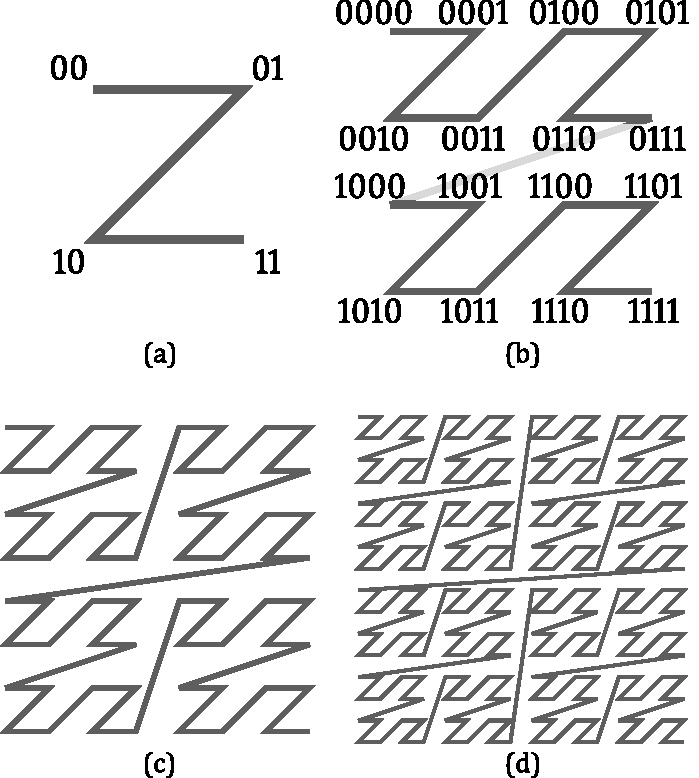
\includegraphics[width=0.65\textwidth]{morton-multiple.pdf}
	\caption[Four resolutions of Morton codes]{
		The first four resolutions of Morton codes for a quadtree.
		(a)--(d) show resolutions 1--4, respectively.
		Modified from~\cite{morton-multiple}; original image courtesy of David Eppstein -- CC BY-SA 3.0.
	}
	\label{fig:morton-multiple}
\end{figure}


\Cref{fig:morton-multiple} demonstrates Morton coding for four resolutions of a conventional Euclidean quadtree.
Indices are assigned consecutively, starting at zero, to cells in the order the curve passes through them.
The resulting indices are hierarchical, where the index of a cell is that of its parent with its local index---obtained relative to its parent---appended.
While shown for a quadtree (2D), Morton codes generalize to any integer dimension $n$.
In this case, each cell has $2^n$ children, which means $n$ bits are needed to represent each uniquely.
Thus, from a given cell index, the resolution of the grid that cell appears at is the bit width of the index divided by $n$.
For a fixed-width representation of indices, a leaded bit set to one marks the start of the actual index.


\begin{figure}[htp!]
	\centering
	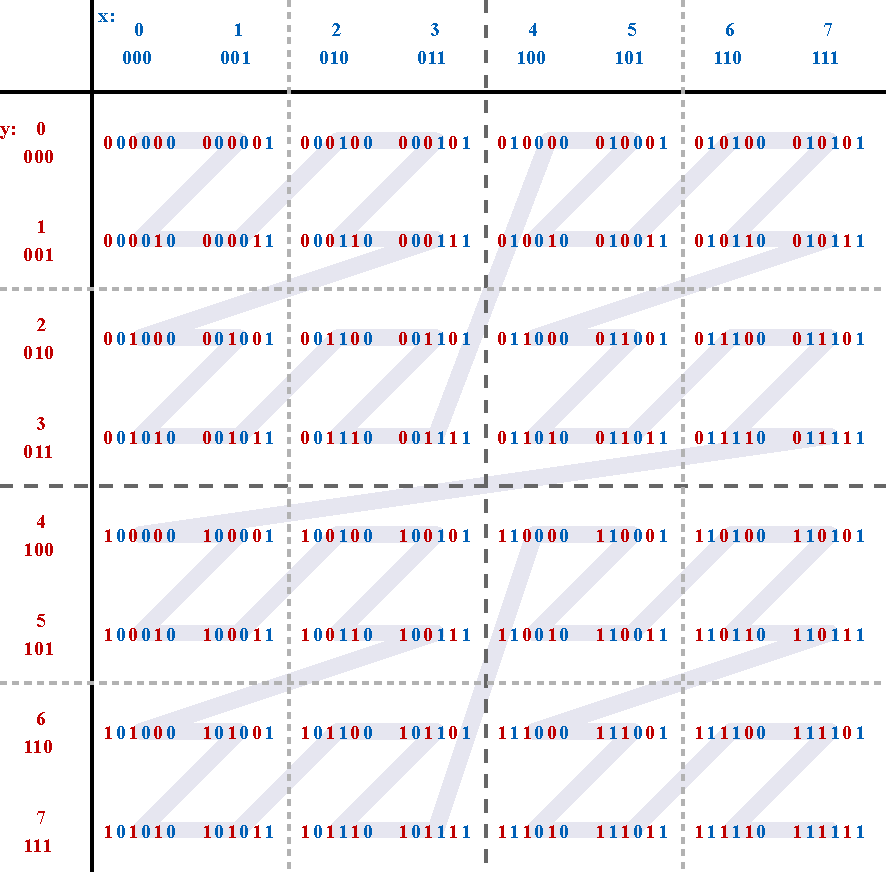
\includegraphics[width=\textwidth]{morton-interleave.pdf}
	\caption[Morton codes by bit-interleaving]{
		Third resolution Morton codes and their respective coordinate indices.
		Note how the Morton codes are obtained by interleaving the bits of the coordinate indices.
		In this figure, the $x$ coordinate is traversed first by the curve, so it is the lowest order bit in the Morton code.
		Image courtesy of David Eppstein~\cite{morton-interleave} -- CC BY-SA 3.0.
	}
	\label{fig:morton-interleave}
\end{figure}


One benefit of Morton codes over more local space-filling curves---such as the Hilbert curve---is the ease at which a multi-dimensional index is encoded and vice versa.
As demonstrated in \cref{fig:morton-interleave}, the Morton code is obtained simply by interleaving the bits of the coordinate indices; likewise, unweaving the bits of a Morton code gives the coordinate indices.
While these are not constant-time operation in general, magic numbers and lookup tables allow them to be done efficiently and in constant time for a fixed bit width~\cite{libmorton18}.
We employ this interleaving and unweaving in our direct coding algorithms for efficient conversion between a combined index and coordinate indices.


\begin{figure}[ht!]
	\centering
	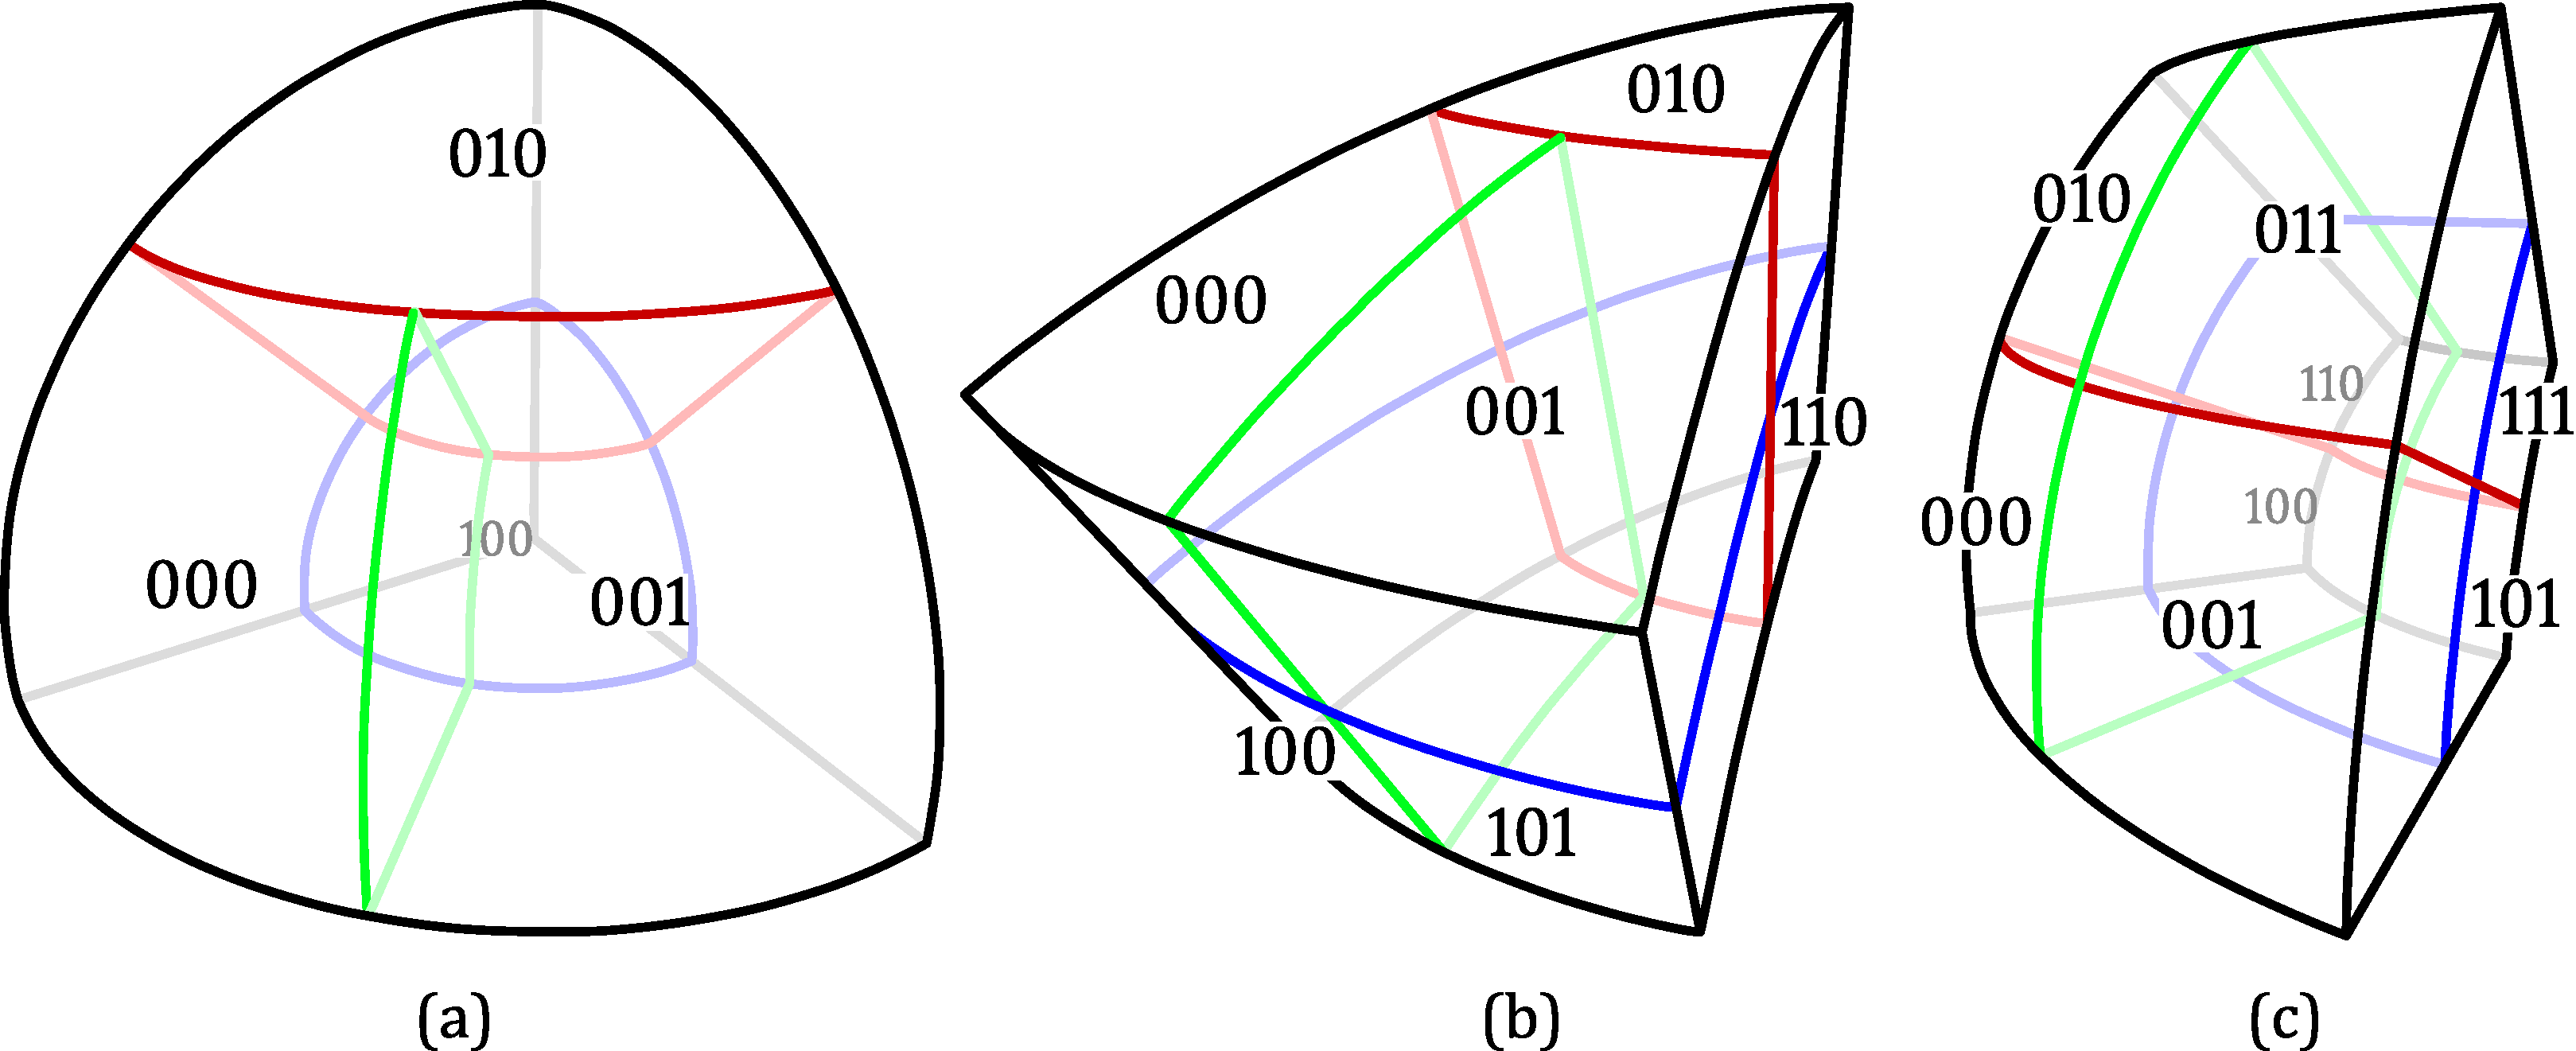
\includegraphics[width=\textwidth]{sdog-dmc.pdf}
	\caption[Degenerate Morton codes for the different SDOG cell types]{
		Degenerate Morton codes for (a) SG cells, (b) LG cells, and (c) NG cells
	}
	\label{fig:sdog-dmc}
\end{figure}


While Morton codes have many desirable properties, due to the semiregular degenerate nature of SDOG, they must be modified for use with the grid system.
First, we apply Morton coding for a cell's children as if refinement was entirely regular.
For NG cells, refinement \textit{is} regular, and no modifications are needed.
However, for SG and LG cells, some of these codes will refer to the same cell.
In these cases, we merge duplicate codes with the lower value kept.
We call this the degenerate Morton code (DMC).
\Cref{fig:sdog-dmc} shows the child codes of cells for each SDOG cell type.
In this scheme, the different spherical coordinates are traversed in the order (1) longitude---small to large (2) latitude---small to large (3) radius---large to small.
Finally, to distinguish between the eight octants, each is given a unique identifier: the octant code.
The full index of an SDOG cell consists of the octant code and DMC, concatenated, along with a leading one for fixed-width representations.
For the remainder of this chapter, we assume the use of a fixed-width integer for representing SDOG indices.
From this definition, we know the number of bits needed to represent an SDOG index at refinement level $k$ is $3k + 4$.
Likewise, given an index with width $\omega$, the refinement level of that cell is $(\omega - 4) / 3$.
We use this property to implicitly obtain $k$ in any case where it is not provided.


It is worth noting that because DMC combines codes for degenerate cells, not every integer is a valid index.
For DMC, the utilization of indices is approximately 38\% of all possible values ($8/21$ in the limit).
Compared to an indexing scheme that uses every possible integer as an index (maximal), DMC based indexing for SDOG requires more bits to index the same level of refinement.
However, if using a fixed-width representation of indices, this is only a downside if the size of the integer cannot support the needed resolution; in this case, a maximal index could potentially allow representing a higher level of refinement.
For a 64 bit integer, though, the maximum level of refinement for both DMC based indexing and a maximal one is 21.
Furthermore, 128 bits provided enough indices for 41 levels of refinement with DMC, at which point the size of cells in on the order of micrometres.
For these reasons, we believe the wasted indices are not a significant issue with DMC indexing in practice.


\subsection{Hierarchical Algorithms}
We first give a brief overview of the hierarchical coding algorithms for SDOG, as these are the baseline for evaluating our proposed ones.
Hierarchical coding works by traversing the grid system one resolution at a time, using the refinement rules for the relevant cell at each iteration.
As a result, these types of algorithms are linear on the level of refinement.
Furthermore, because they use refinement rules directly, they are trivially modified to work for our SDOG modifications by simply changing the refinement used in the algorithms accordingly.


\subsubsection{Encoding}
The algorithm for hierarchical point encoding with SDOG is given in \cref{alg:encode}.
The input is a point $p$ and resolution $k$; the output is the index $i$ of the cell that contains $p$ at $k$.


\begin{algorithm}[htp!]
	\caption{Hierarchical point encoding for SDOG}
	
	\begin{algorithmic}
		
		\STATE determine which octant contains $p$
		\STATE cellBoundaries $\leftarrow$ boundaries of octant
		\STATE currCellType $\leftarrow$ SG
		\STATE $i \leftarrow \operatorname{append}(1, \mathrm{octantCode})$
		
		\FOR{$k$ iterations}
		\STATE use refinement rules for currCellType with cellBoundaries to find child cells
		\STATE determine which child contains $p$
		\STATE cellBoundaries $\leftarrow$ boundaries of child
		\STATE currCellType $\leftarrow$ type of child
		\STATE $i \leftarrow \operatorname{append}(i, \mathrm{child~index})$
		\ENDFOR
		\RETURN $i$
		
	\end{algorithmic}
	\label{alg:encode}
\end{algorithm}


\subsubsection{Decoding}
The algorithm for hierarchical decoding with SDOG is given in \cref{alg:decode}.
The input is an index $i$; the output is the cell boundaries of $i$.


\begin{algorithm}[htp!]
	\caption{Hierarchical cell decoding for SDOG}
	
	\begin{algorithmic}
		
		\STATE determine octant from $i$
		\STATE cellBoundaries $\leftarrow$ boundaries of octant
		\STATE currCellType $\leftarrow$ SG
		\STATE remove highest four bits of $i$
		
		\FOR{$k$ iterations}
		\STATE use refinement rules for currCellType with cellBoundaries to find child cells
		\STATE $c \leftarrow$ highest three bits of $i$
		\STATE remove highest three bits of $i$
		\STATE determine which child cell matches $c$
		\STATE cellBoundaries $\leftarrow$ boundaries of $c$
		\STATE currCellType $\leftarrow$ type of $c$
		\ENDFOR
		\RETURN cellBoundaries
		
	\end{algorithmic}
	\label{alg:decode}
\end{algorithm}


\subsection{Direct Algorithms}
While hierarchical algorithms are straightforward and simple to implement, their linear runtime means they are inefficient for high values of $k$.
Instead, the uniform refinement of SDOG can be leveraged for direct version of encoding and decoding.
We introduce modifications of conventional direct indexing methods to work for SDOG.


For a uniform grid, the coordinate indices of the cell that contain a point are obtained trivially in constant time.
Likewise, the maximum and minimum coordinates of a cell are also easily computed from a coordinate index.
For these operations, the necessary variables are the number of cells ($n$) and the range of values in each coordinate dimension.
Let $\hat{c}$ be a coordinate value normalized withing the respective range, then the coordinate index of the cell containing $\hat{c}$ is $c_i = \lfloor \hat{c} \cdot n \rfloor$.
Similarly, the normalized maximum and minimum coordinate values of a cell are obtained from the index with
$\hat{c}_\mathrm{max} = (c_i + 1) / n$ and $\hat{c}_\mathrm{min} = c_i / n$, respectively.


We know that the semiregular regions of SDOG are uniform when using conventional refinement rules.
Therefore, if we determine the relevant semiregular region and its needed properties---the number of cells and range of values---we can apply direct coding algorithms for SDOG using spherical coordinates (refer back to \cref{fig:sph-elements}).
Then, bit interleaving and unweaving give the full DMC.
In SDOG, the number of cells in the different coordinate dimensions varies for different regions of the grid.
Under regular refinement, the number of cells in each coordinate dimension at $k$ levels of refinement is $2^k$.
Each increasing shell in SDOG halves the number of cells in the latitude and longitude coordinates.
Furthermore, each increasing zone further halves the number of cells in the longitude coordinate.
Since a DMC is relative to an octant, the range of coordinate values for direct coding are the ranges of the octant itself.
Therefore, all that we need for direct coding is the shell and zone that contain the point or cell being considered.


\subsubsection{Encoding}
The inputs and outputs of direct encoding are the same as its hierarchical counterpart.
First, we find the octant that contains $p$.
The three coordinates of $p$ are then normalized within the range of the octant with $\hat{r} = r / R_\mathrm{max}$, $\hat{\varphi} = \pm (2\varphi) / \pi$, and $\hat{\lambda} = 2 (\lambda - \lambda_0) / \pi$, where $\lambda_0$ is the minimum longitude of the octant.
We then calculate the shell and zone that contain $p$ the same as in \cref{chap:mapping}: $s = \lfloor \log_{0.5} \hat{r} \rfloor$ and $z = \lfloor \log_{0.5} ( 1 - \hat{\varphi} ) \rfloor$.


The number of latitude division is $2^k$ divided by $2^s$; however, the number of divisions is always at least one.
Thus, we introduce variable $k_\varphi = \min ( s, k )$.
Similarly, the number of longitude division is $2^k$ divided by $2^{s+z}$, but again, is always at least one.
We introduce a second variable $k_\lambda = \min ( s + z, k )$.
Finally, we calculate coordinate indices, making sure to account for the direction of each coordinate in the DMC for SDOG.
Let the subscript $i$ refer to the index the coordinate, then
%
\begin{equation*}
r_i = 2^k \cdot ( 1 - \hat{r} ),
\end{equation*}
%
\begin{equation*}
\varphi_i = 2^{k - k_\varphi} \cdot \hat{\varphi}, \quad \text{and}
\end{equation*}
%
\begin{equation*}
\lambda_i = 2^{k - k_\lambda} \cdot \hat{\lambda}.
\end{equation*}
%
The DMC, then, is the Morton interleaving of $\lambda_i$, $\varphi_i$, and $r_i$ (in that order); the full index is the octant code and DMC concatenated with the preceding bit set.


\subsubsection{Decoding}
The inputs and outputs of the direct decoding are the same as its hierarchical counterpart.
First, we get the octant code and DMC from $i$.
The DMC is then unwoven to get the coordinate indices $\lambda_i$, $\varphi_i$, and $r_i$.


We now decode the coordinate indices one at a time.
As the number of radial division is never modified, we start by decoding the radial index: 
%
\begin{equation*}
\hat{r}_\mathrm{max} = 1 - \frac{r_i}{2^k} \quad \text{and}
\end{equation*}
%
\begin{equation*}
\hat{r}_\mathrm{min} = 1 - \frac{r_i + 1}{2^k}.
\end{equation*}
%
With this, we can now determine the shell that contains the cell being decoded.
We use $\hat{r}_\mathrm{max}$ as opposed to $\hat{r}_\mathrm{min}$, as the latter gives the inner shell if on the boundary. Thus, $s = \lfloor \log_{0.5} \hat{r}_\mathrm{max} \rfloor$.
Just as with encoding, we define $k_\varphi = \min ( s, k )$.
We now have the needed information to decode latitude:
%
\begin{equation*}
\hat{\varphi}_\mathrm{max} = \frac{\varphi_i + 1}{2^{k - k_\varphi}} \quad \text{and}
\end{equation*}
%
\begin{equation*}
\hat{\varphi}_\mathrm{min} = \frac{\varphi_i}{2^{k - k_\varphi}}.
\end{equation*}
%
Likewise, we can now determine the zone that contains the cell.
Opposite of radius, $\hat{\varphi}_\mathrm{max}$ now gives the higher zone if on the boundary, so we use $\hat{\varphi}_\mathrm{min}$ and get $z = \lfloor \log_{0.5} ( 1 - \hat{\varphi}_\mathrm{min} ) \rfloor$.
Again, the same as encoding, we define $k_\lambda = \min ( s + z, k )$.
Finally, we decode longitude:

% intentional break for typesetting spacing

\begin{equation*}
\hat{\lambda}_\mathrm{max} = \frac{\lambda_i + 1}{2^{k - k_\lambda}} \quad \text{and}
\end{equation*}
%
\begin{equation*}
\hat{\lambda}_\mathrm{min} = \frac{\lambda_i}{2^{k - k_\lambda}}.
\end{equation*}
%
The last step is to get the bounds of the octant from the octant code and convert the normalized values to actual ones.


\subsubsection{For Modified SDOG}
These direct algorithms only work for conventional SDOG due to the requirement of uniform spacing of grid divisions.
As described in \cref{chap:mapping}, however, the mapping functions allow these algorithms to be used with the modified grids by mapping them to conventional SDOG.
For encoding, the point $p$ must be forward mapped before encoding, making the full operation $\operatorname{encode}(M(p))$.
For decoding, the output ranges must be inverse mapped after decoding, making the full operation $M^{-1}(\operatorname{decode}(i))$.
In both cases, there is overlap in the computations done by the coding algorithm and associated mapping functions (e.g. calculating $s$ and $z$), so care should be taken during implementation to avoid redundant computations.


\subsection{Runtime Comparison} \label{chap:7:runtime}
To evaluate the usefulness of our direct coding algorithms, we compare their runtime against the hierarchical counterparts.
To do so, we have implemented the four algorithms and the mapping functions presented in \cref{chap:mapping} in C++.
We also used these implementations to experimentally verify the correctness of the direct algorithms by comparing their output to the hierarchical ones.


The combination of two algorithmic approaches (hierarchical vs. direct) and four grids (SDOG and the three modifications in \cref{chap:sdog}) result in eight total algorithms to compare for both encoding and decoding.
For simplicity, we only benchmark the DMC portion of coding.
First, we generate one million points randomly distributed within an SDOG octant.
For each resolution being benchmarked, we then time each of the encoding algorithms using the generated points.
The resulting indices are then used to time each of the decoding algorithms in the same manner.
We time resolutions $1 \le k \le 21$, as 21 is the highest resolution \textit{without} an octant code that can be represented by a 64-bit integer.
We use the Libmorton library~\cite{libmorton18} to perform efficient bit-interleaving and unweaving.


\begin{figure}[htp!]
	\centering
	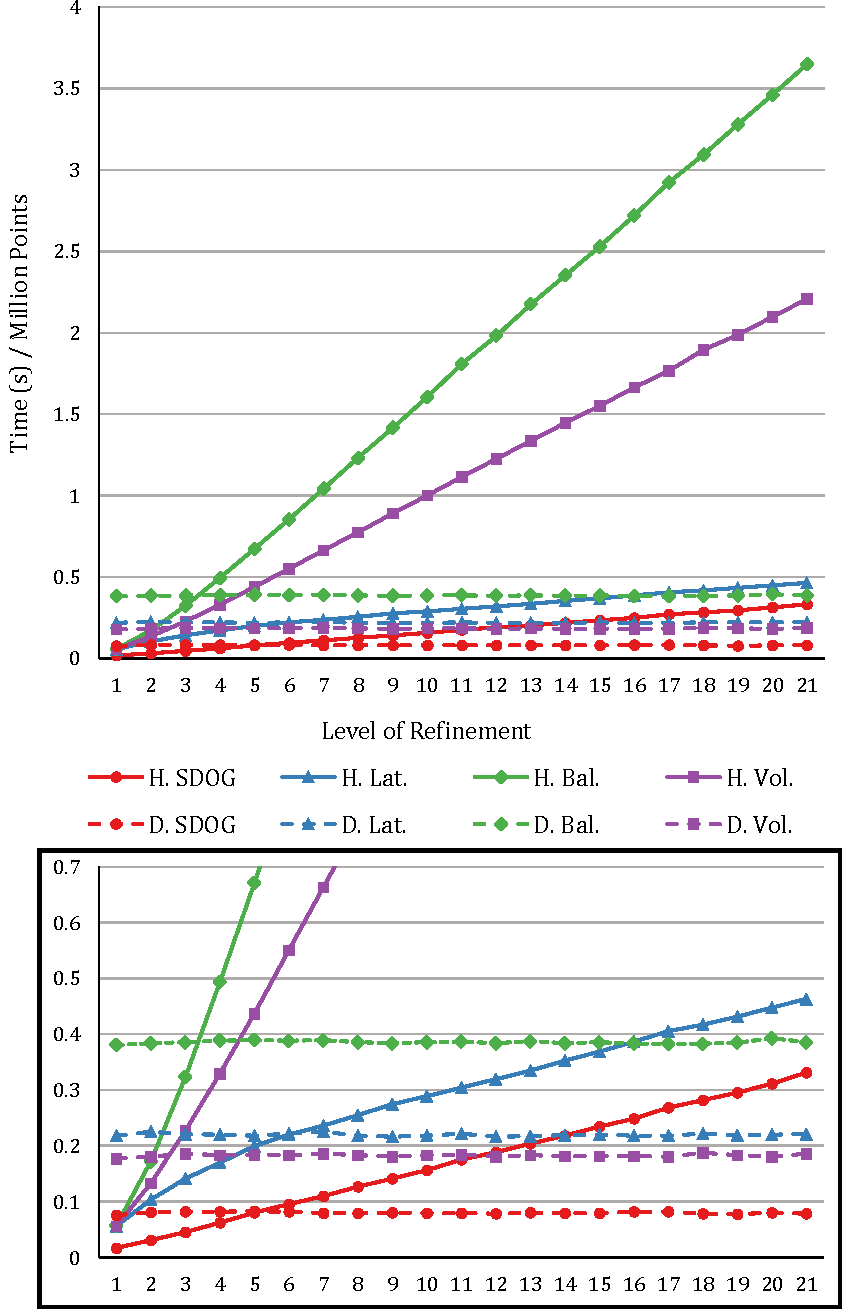
\includegraphics[width=0.8\textwidth]{point-to-index.pdf}
	\caption[Runtime comparison of SDOG point encoding algorithms]{
		Runtime of the hierarchical (H) and direct (D) encoding algorithms for SDOG and our proposed modifications (Lat = Latitude, Bal = Balanced, and Vol = Volume).
		The bottom chart is the same as the top but with a smaller vertical scale to better compare values.
	}
	\label{fig:point-to-index}
\end{figure}


\begin{figure}[htp!]
	\centering
	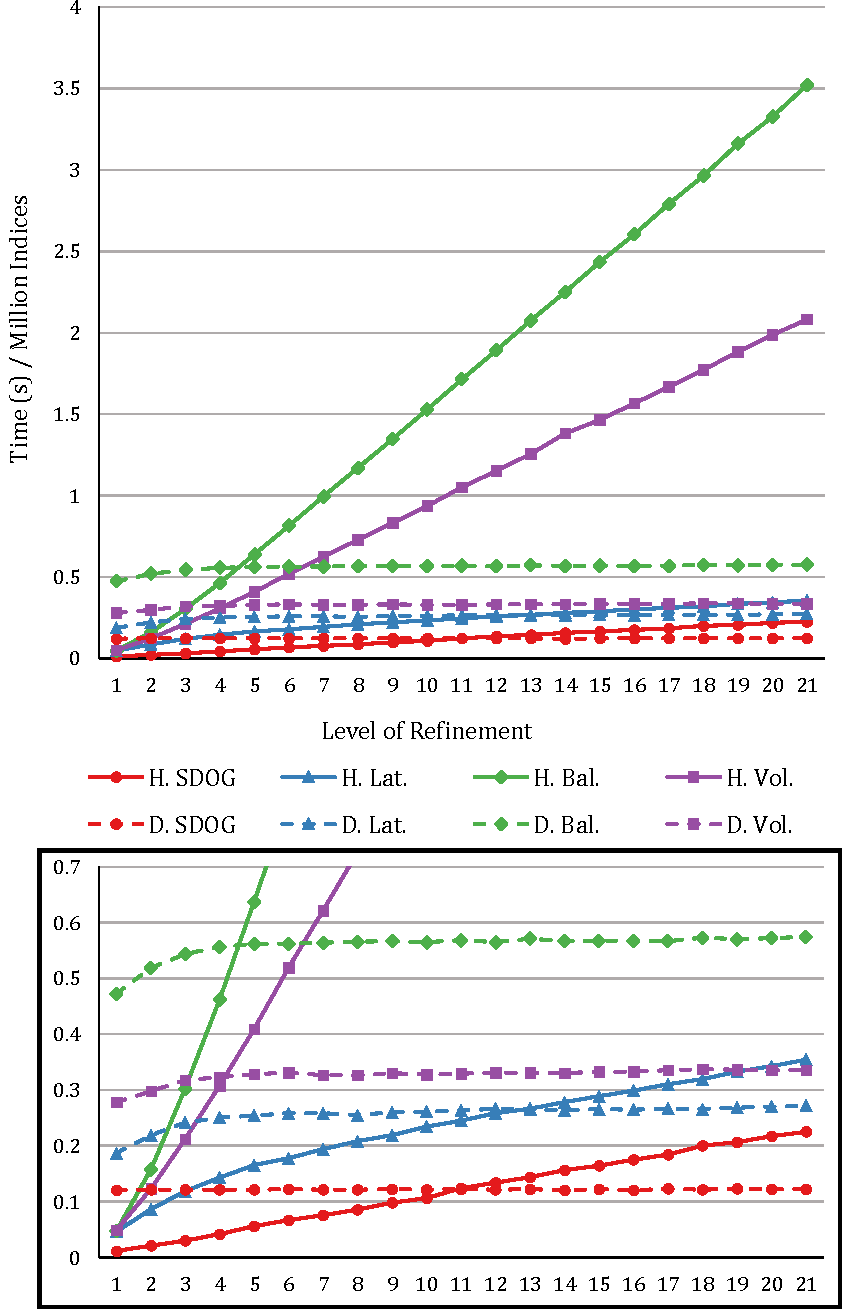
\includegraphics[width=0.8\textwidth]{index-to-range.pdf}
	\caption[Runtime comparison of SDOG decoding algorithms]{
		Runtime of the hierarchical (H) and direct (D) decoding algorithms for SDOG and our proposed modifications (Lat = Latitude, Bal = Balanced, and Vol = Volume).
		The bottom chart is the same as the top but with a smaller vertical scale to better compare values.
	}
	\label{fig:index-to-range}
\end{figure}


\Cref{fig:point-to-index,fig:index-to-range} show the benchmarking results for encoding and decoding, respectively.
In order to reduce noise, these charts show the average of two evaluations of the benchmarking.
As is expected, the hierarchical algorithms are linear on $k$ and the direct algorithms (mostly) constant on $k$.


For the hierarchical algorithms, the difference in runtime between the different grids is determined by the complexity of calculating splitting surfaces for cells.
For hierarchical encoding and decoding, SDOG is the most efficient closely followed by the latitude method; the volume method is significantly slower than these two, and the balanced method significantly slower than the volume one.
For the direct algorithms, this difference is determined by the complexity of evaluating the mapping functions.
For direct encoding, SDOG is most efficient, then volume closely followed by latitude, and then balanced.
Decoding is slightly different, with latitude and volume swapping places in the ordering.


In general, the hierarchical decoding algorithms are slightly quicker than their encoding counterparts.
The reasons for this are not entirely clear; however, it seems to imply that determining which child cell contains a point is slightly more expensive than setting the child cell dimensions based on a given code.
For the direct algorithms, the opposite holds, and the encoding algorithm is the quicker of the two.
The reason for this is the encoding algorithm only computes three values (an index for each coordinate), whereas the decoding must compute twice as many (a maximum \textit{and} minimum for each coordinate).
Furthermore, for the modified grids using the mapping functions, this means that decoding also requires twice as many uses of these functions.


Overall, the direct algorithms are all more efficient than their hierarchical counterpart for a large enough value of $k$.
Thus, a sophisticated implementation could determine which approach to use (hierarchical or direct) for a given input, depending on $k$.
However, benchmarking on a variety of platforms in different conditions would be needed to determine the best values to use for the switch.
\Cref{tab:hierarch-vs-direct} summarizes the lowest value of $k$ such that the direct algorithm is more efficient than the hierarchical for each pair of algorithms in \textit{our} benchmarks.


\begin{table}[htp!]
	\centering
	\caption[Resolution at which direct coding becomes more efficient than hierarchical]{
		The resolution ($k$) at which our direct coding algorithms become more efficient than their hierarchical counterparts
	}
	\begin{tabular}{@{} c c c c c @{}}
		\toprule
		         & SDOG & Latitude & Balanced & Volume \\ \midrule
		Encoding & 6    & 7        & 4        & 3      \\
		Decoding & 11   & 13       & 5        & 5      \\ \bottomrule
	\end{tabular}
	\label{tab:hierarch-vs-direct}
\end{table}


A final note is that runtime for direct decoding of the modified grids grows until about resolution four, where it then levels off to constant.
The reason for this is subtle.
In the decoding algorithm, values of $s$ and $z$ are calculated from the bounds of the cell being decoded.
Therefore, their values are bounded by $k$.
However, $s$ and $z$ are used as exponents when calculating $\ell$ and $u$ values, and in many implementations, calculating powers is faster for lower exponents (specifically, exponents of zero, one, and two).
Thus, low values of $k$ have lower maximum (and average) exponents and, therefore, slightly lower runtime.
This same effect does not appear in the encoding algorithms since $s$ and $z$ are calculated directly from $p$ with no respect to $k$.


\subsection{Other Indexing Operations}
Since the SDOG indexing described above is based on coordinate indices, grid traversal queries are mostly straightforward.
However, the nature of semiregular degenerate refinement introduces a few complications that make parent, child, and neighbour operations more complex than the respective operations in a perfectly regular grid.
We briefly describe how to perform each of these for a given SDOG index, $i$, below.


\paragraph{Parent:}
The use of Morton interleaving makes parent queries trivial. The parent of $i$ is simply $i$ with the lowest three bits removed.


\paragraph{Children:}
The children of an SDOG cell depend on the cell type.
A cell is SG if $r_i = 2^k - 1$, LG if $\varphi_i = 2^{k - k_\varphi} - 1$, and is NG otherwise.
Let $C$ be the set of child codes for the cell type of $i$ (refer to \cref{fig:sdog-dmc}), then the children of $i$ are $\{ \operatorname{append}(i, c) \ | \ c \in C \}$


\paragraph{Neighbours:}
Neighbours are by far the most complicated of the three operations due to the number of edge cases that need be handled.
First, we obtain the coordinate indices of $i$ just as with decoding.
In general, the coordinate indices of the neighbours of an SDOG cell are $\{ (\lambda_i', \varphi_i', r_i') \ | \ x' \in x \pm 1 \}$, which are then interleaved and combined with the octant code for the full index.
However, specific cells in SDOG require a modified formulation for certain neighbours.
Special care is needed for cells that border the edge of an octant or the boundaries of shells and zones.
Below we list how to detect these cases and how to modify the neighbour calculation accordingly; cases 1--4 handle octant boundaries and 5--8 handle shell and zone boundaries.
%
\begin{enumerate}
	\item If $\lambda_i = 2^{k - k_\lambda} - 1$, then $\lambda_i + 1$ is in a neighbouring octant.
	For this neighbour, set $\lambda_i' = 0$ and use the octant code for the neighbouring octant.
	\item If $\lambda_i = 0$, then $\lambda_i - 1$ is in a neighbouring octant.
	For this neighbour, set $\lambda_i' = 2^{k - k_\lambda} - 1$ and use the octant code for the neighbouring octant.
	\item If $\varphi_i = 0$, then $\varphi_i - 1$ is in a neighbouring octant.
	For this neighbour, set $\lambda_i' = 0$ and use the octant code for the neighbouring octant.
	\item If $\varphi_i = 2^{k - k_\varphi} - 1 - 1$, $r_i = 2^k - 1$, or $r_i = 0$, then the cell is on the boundary of the octant with no neighbours in the corresponding direction (increasing, increasing, and decreasing, respectively).
	\item If $\varphi_i = 2^n - 1$ for some $n \in \mathbb{Z}$, then $\varphi_i + 1$ is in the next spherical zone, which has half as many longitude divisions.
	For this neighbour, set $\lambda_i' = \lfloor \lambda_i / 2 \rfloor$.
	\item If $\varphi_i = 2^n$ for some $n \in \mathbb{Z}$, then $\varphi_i - 1$ is in the previous spherical zone, which has twice as many longitude divisions.
	In this case, there are two neighbours in this direction; set $\lambda_i' = 2 \lambda_i, \  2 \lambda_i + 1$.
	\item If $r_i = 2^n - 1$ for some $n \in \mathbb{Z}$, then $r_i + 1$ is in the next spherical shell, which has half as many longitude and laitude divisions.
	For this neighbour, set $\lambda_i' = \lfloor \lambda_i / 2 \rfloor$ and $\varphi_i' = \lfloor \varphi_i / 2 \rfloor$.
	\item If $r_i = 2^n$ for some $n \in \mathbb{Z}$, then $r_i - 1$ is in the previous spherical shell, which has twice as many longitude and latitude divisions.
	In this case, there are four neighbours in this direction; set $\lambda_i' = 2 \lambda_i, \  2 \lambda_i + 1$ and $\varphi_i' = 2 \varphi_i, \  2 \varphi_i + 1$.
\end{enumerate}
%


\section{Extension Method} \label{chap:7:extension}
For our grid extension method, encoding and decoding operations are defined for the input DGGS and should be leveraged when defining the 3D version of these operations.
Doing so not only simplifies the definition of these operations (by deferring work to the input DGGS) but also facilitates the simple transference of data between the input DGGS and its 3D counterpart.
To accomplish this, we split encoding and decoding into a surface and radial component.
Referring to \cref{fig:prismatoid-indexing}, we justify such a split by noting that two components define each cell in a 3D DGGS: the cell of the input DGGS that defines its base(s) and the layer of the grid that contains it.
Uniquely identifying each of these components is sufficient to identify every cell in the grid uniquely; furthermore, each of these components is determined almost entirely independently of one another.


\begin{figure}[htp!]
	\centering
	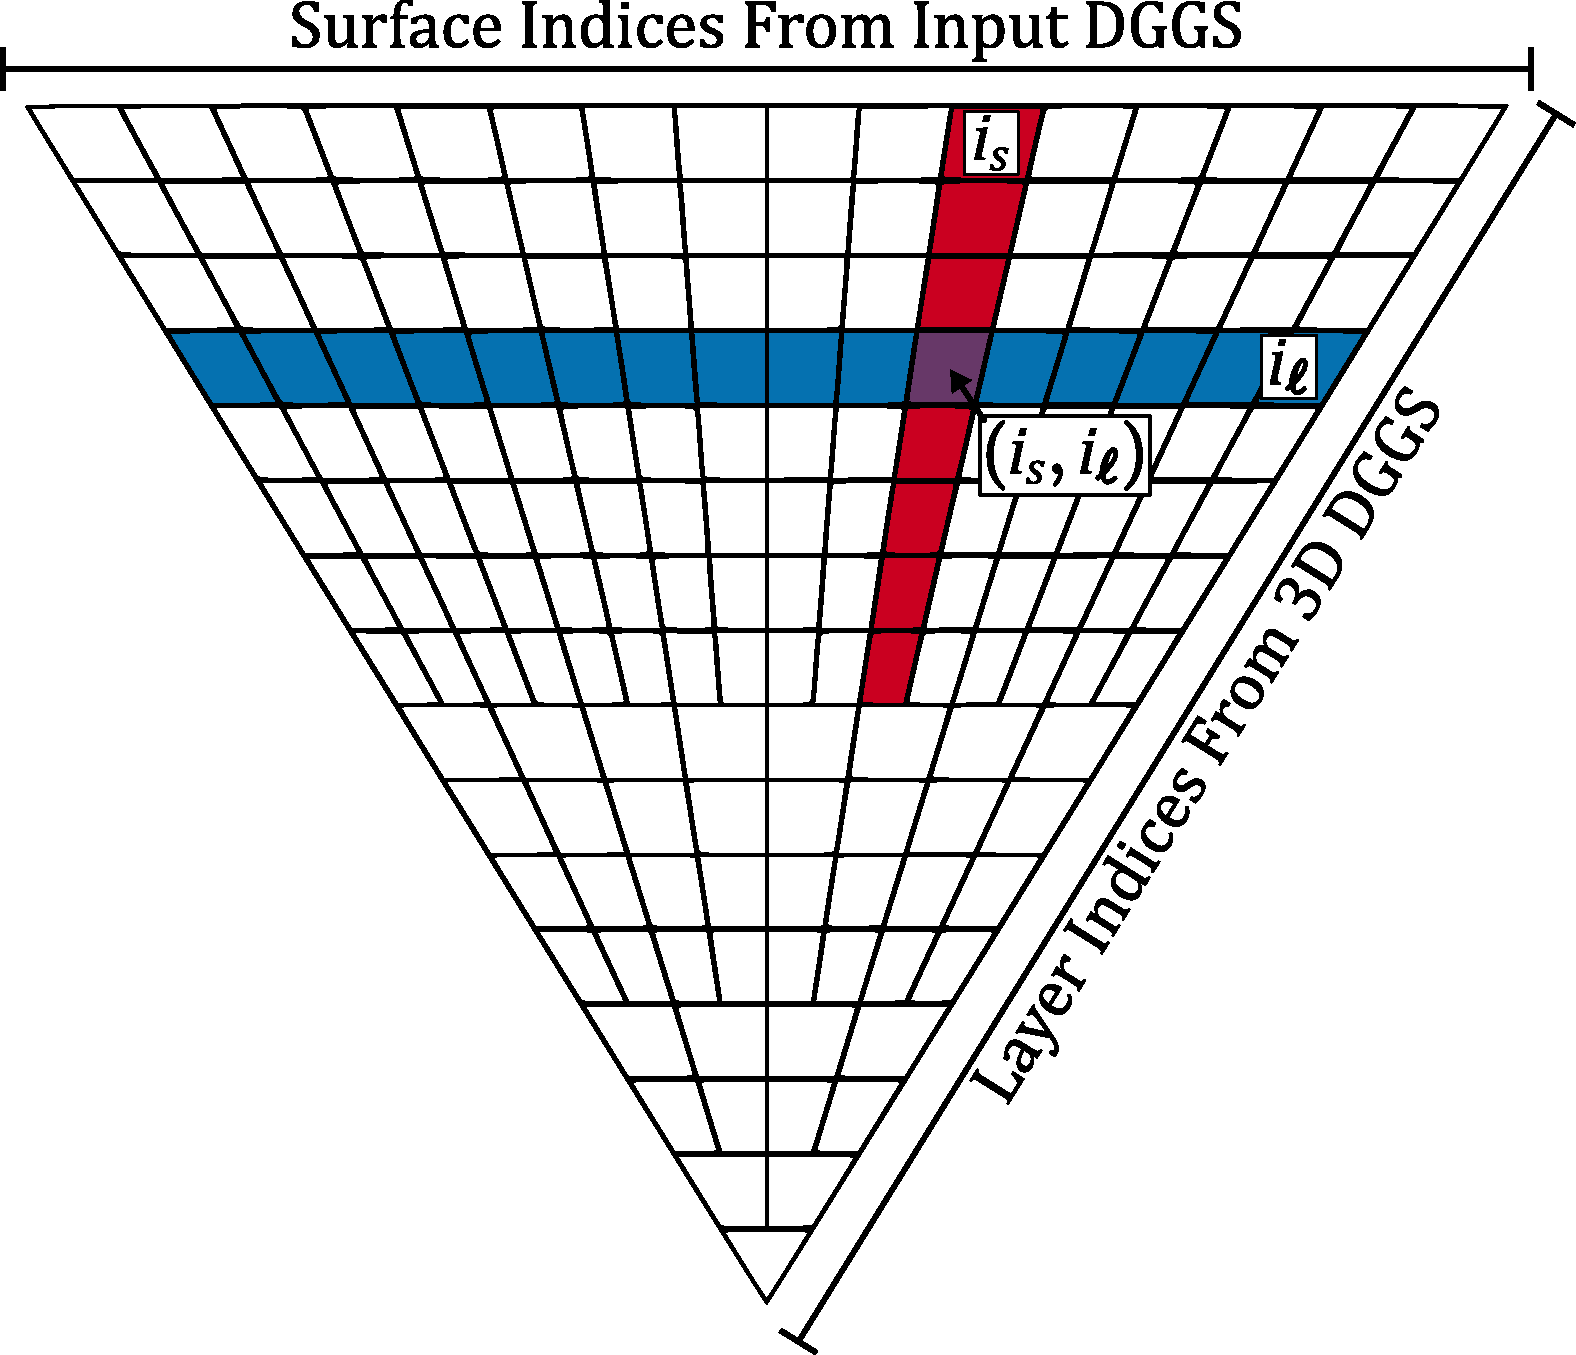
\includegraphics[width=0.6\textwidth]{prismatoid-indexing.pdf}
	\caption[Separation of surface and layer indices for the grid extension method]{
		Indices from the input DGGS identify cells in the 3D DGGS with the same bases but different radii.
		Likewise, each layer of the 3D DGGS contains all cells with the same radii but different bases.
		Thus, these two pieces of information combined are sufficient to identify any cell in the 3D DGGS uniquely.
		Here, we show a single cell---highlighted in purple---along with all the cells that share a surface index (red) and a layer index (blue).
	}
	\label{fig:prismatoid-indexing}
\end{figure}


\begin{figure}[htp!]
	\centering
	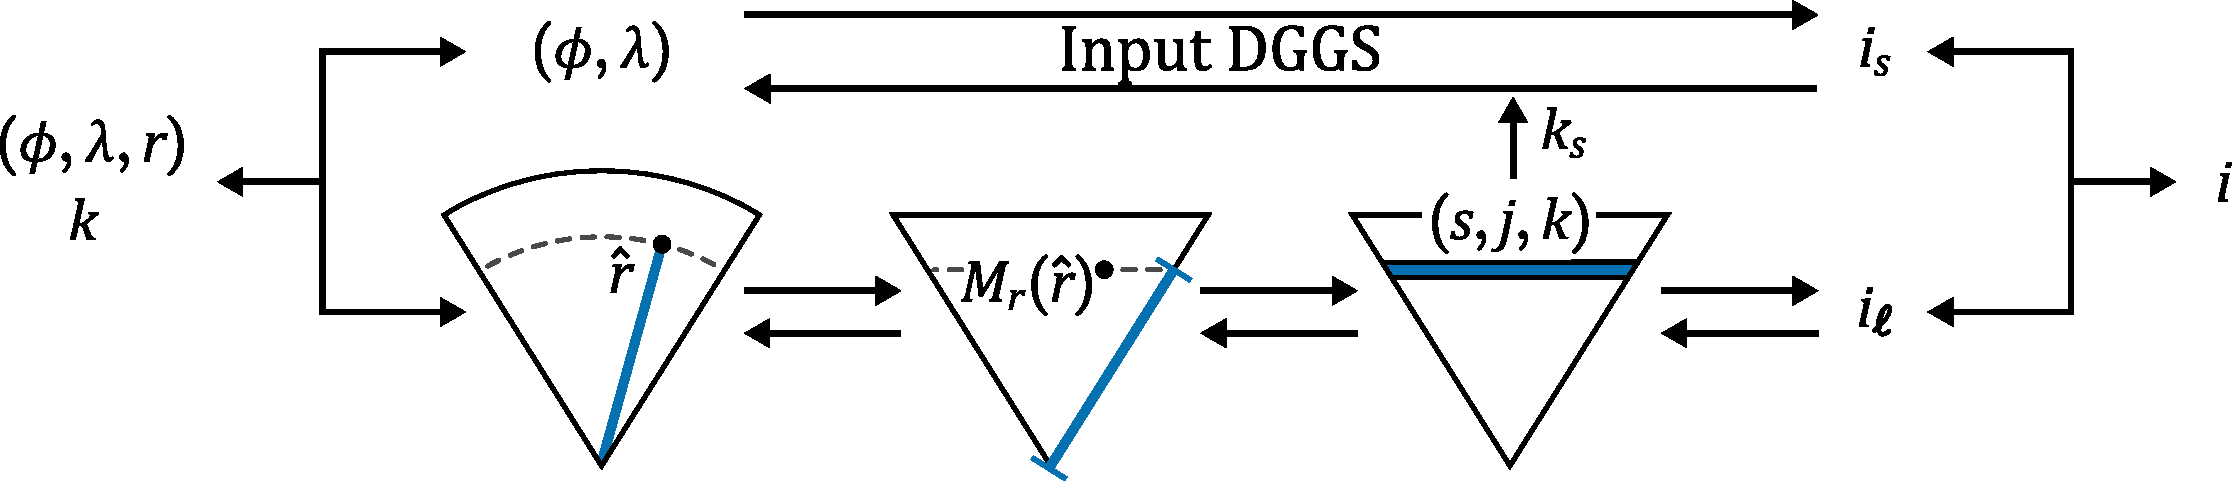
\includegraphics[width=\textwidth]{3d-coding.pdf}
	\caption[Pipeline for encoding and decoding with the grid extension method]{
		Pipeline for splitting encoding and decoding into surface (top) and radial (bottom) components.
		These two components are entirely independent except for the surface resolution ($k_s$) of the layer being provided to the surface component during encoding.
		Refer to \cref{chap:6:radial} for details on the mapping function ($M_r$) used in the radial component.
	}
	\label{fig:prismatoid-coding}
\end{figure}


\Cref{fig:prismatoid-coding} illustrates the pipeline for our proposed split of these operations.
The surface component of coding is handled entirely by the input DGGS and, therefore, is not discussed here.
For the radial component, encoding and decoding make use of the forward and inverse radial mapping functions provided in \cref{chap:6:radial}, respectively.
We also provide a parameterization for identifying the layers of a 3D DGGS, and operations for encoding and decoding this parameterization.
To maintain the generality of our algorithms, we work exclusively with this parameterization instead of discussing techniques for linearizing it into a single index.
We do so because the varying complexity of the layer structure in a 3D DGGS---combined with the competing goals of an indexing scheme---makes defining a general method for linearization challenging.
Similarly, combining layer and surface indices into a single index depends heavily on the input DGGS and should respect the priorities (e.g. good locality, maximum efficiency) of its indexing scheme, and therefore, is also difficult to do in general.





Layers of our 3D DGGS's can be parameterized by the shell they reside in ($s$), the integer index of the layer relative to the shell ($j$), and the level of refinement ($k$); we denote the central layer with $s = -1$.
Thus, layer encoding calculates these values from $\hat{r}$ and layer decoding calculates $\hat{r}_\mathrm{max}$ and $\hat{r}_\mathrm{min}$ from these values.


\subsection{Encoding}
The level of refinement $k$ is an input into encoding; therefore, only the shell $s$ and the integer index $j$ need to be computed.
The value of $s$ is carried forward from the radial mapping function evaluation.
In order to calculate $j$, the number of layers in the shell is first needed; this depends on the refinement level, the layering sequence, and the number of extra radial splits (see \cref{chap:extension}).
The refinement level is an input, and the other variables are constant for any given 3D DGGS.
The number of layers is
%
\begin{equation*}
n_\ell = \left( x+1 \right) \prod_{i = s}^{k - 1} \ell_i.
\end{equation*}
%
Recall that $\ell_i$ refers to the number of layer produced when refining normal layers at refinement level $i$, which is unrelated to the values $\ell_g$ and $\ell_p$.
In the case where $s$ is greater than $k-1$, the shell is in the central layer.
In this case, we set $s = -1$ and $j = 0$.
The integer index of the layer is then $j = \lfloor d \cdot n_\ell \rfloor$, where $d$ is carried forward from the radial mapping function.
Finally, as input into the surface encoding, the value of $k_s$ is needed for the shell.
For central layers, this is always zero; otherwise, it is $k - s - 1 + w$.


Note that only the values of $s$ and $d$ are used in the above calculation and \textit{not} $\hat{r}$.
Therefore, the full evaluation of the radial mapping is unnecessary, and only \cref{eq:radialForwD} is evaluated for encoding.


\subsection{Decoding}
For decoding, we calculate $d_\mathrm{min}$ and $d_\mathrm{max}$ as $j/n_\ell$ and $(j+1)/n_\ell$, respectively.
These values are then fed directly into the inverse radial mapping as values of $d$ in \cref{eq:radialInv}.


\subsection{Other Indexing Operations}
Similar to encoding and decoding, we define grid traversal operations in terms of surface and radial components.
Referring back to \cref{fig:prismatoid-indexing,fig:prismatoid-coding}, we let $i_s$ be the surface index of a cell and $i_\ell$ be the layer index.
For each of these components, we assume there is a corresponding parent(s), child, and neighbour operation.
For the surface index, this comes directly from the input DGGS indexing, whereas for the layer index, we define these in terms of the layer parameterization provided above.


\subsubsection{Layer Operations}
For each of the operations, we describe how to calculate the output layer parameterization(s) $(s',j',k')$ from that of the input layer $(s,j,k)$.


\paragraph{Parent:}
Trivially, the parent layer is in the previous resolution of the 3D DGGS, so $k' = k - 1$.
For calculating $s$ and $j$, there are two cases, which correspond with the parent layer being central or normal.
If $s = k-1$ or $s = -1$, then the parent layer is a central layer. In this case, $s' = -1$ and $j' = 0$.
Otherwise, the parent layer is normal with $s' = s$ and $j' = \lfloor j / \ell_k \rfloor$.


\paragraph{Children:}
The child layers depend on if the layer in question is central or normal.
Regardless, in both cases all children will have $k' = k + 1$.
Recall that $s = -1$ denotes that a given layer is central.
In this case, one child is the child central layer with $s' = -1$ and $j = 0$.
There are also a number of child normal layers equal to one plus the number of extra radial splits ($x$), given by $s' = s = k$ and $j' = \{ o \in \mathbb{Z} \ | \ o \in [0, x] \}$.
For normal layers, the children are found with $s' = s$ and $j' = \{ j \cdot \ell_k + o \ | \  o \in \mathbb{Z}, \ o \in [0, \ell_k - 1] \}$.


\paragraph{Neighbours:}
Neighbour layers are the layers above and below a given layer; they are at the same resolution, so $k' = k$.
In most cases, the two neighbours are simply given by $s' = s$ and $j' = j \pm 1$; however, there are three edge cases that need to be handled.
If $j = n_\ell - 1$, then the layer above is in the previous shell with $s' = s - 1$ and $j' = 0$; if $s - 1$ is negative, however, then the layer is on the boundary of the grid and there is no layer above it.
If $j = 0$ then the layer below is in the next shell with $s' = s + 1$ and $j' = n_\ell$, where $n_\ell$ is calculated with respect to the new shell (i.e. $s'$).
Finally, the central layer ($s = -1$) has no layer below it and the layer above it has $s' = k - 1$ and $j' = 0$.


\subsubsection{Combined Operations}
With the surface and layer operations defined, we now give the full 3D ones.


\paragraph{Parents:}
The parent(s) of a cell depends on if its layer and its parent layer have the same or different values of $k_s$.
Let $i_\ell' = \operatorname{parent}(i_\ell)$; if the value of $k_s$ is the same, then the single parent is simply $(i_s, i_\ell')$.
In most cases, the value of $k_s$ for $i_\ell'$ is some number $m$ (often one, but not always) less than that of $i_\ell$.
In this case, the parent(s) are given by $\operatorname{parents}^m(i_s) \times i_\ell$.


\paragraph{Children:}
The children of a cell depend on if the cell belongs to a central or normal layer.
For normal layers, the set of children is simply $\operatorname{children}(i_s) \times \operatorname{children}(i_\ell)$.
For central layers, the child who belongs to the new central layer must be distinguished from the other child layer(s).
Call the index of the new central layer $c_\ell$; then, this child is given by $(i_s, c_\ell)$.
Let $ N_\ell$ give the set of the other children layer indices (normal layers).
These layers have the surface refinement applied $w$ times, so the resulting children are $\operatorname{children}^w(i_s) \times N_\ell$.


\paragraph{Neighbours:}
We split neighbours into three categories: neighbours in the same layers as the cell, neighbours in the layer above the cell, and neighbours in the layer below the cell.
If a cell belongs to the outermost or innermost (central) layer, then it will not have neighbours in the layer above or below, respectively.
Neighbours in the same layer are simply $\operatorname{neighbours}(i_s) \times i_\ell$.
Let $i_\ell^+$ be the layer above $i_\ell$ and $i_\ell^-$ be the layer below.
If $i_\ell^+$ has the same value of $k_s$ as $i_\ell$, then the single neighbour above is $(i_s, i_\ell^+)$.
In the other case, where the value of $k_s$ for $i_\ell^+$ is some number $m$ greater than that of $i_\ell$, the neighbours are given by $\operatorname{children}^m(i_s) \times i_\ell^+$.
Likewise, if $i_\ell^-$ has the same value of $k_s$ as $i_\ell$, there is one neighbour below given by $(i_s, i_\ell^-)$.
In the case that the value of $k_s$ for $i_\ell^-$ is some number $m$ less than that of $i_\ell$, the neighbours are given by $\operatorname{parents}^m(i_s) \times i_\ell^-$.


\section{Summary}
Several critical operations enable the integration, analysis, and visualization of data in a DGGS.
By providing point encoding, cell decoding, and grid traversal queries for the 3D DGGS's presented earlier in the thesis, we allow them to serve as fully functioning grid systems.
While there exist more advanced DGGS operations, the ones discussed in this chapter are the most fundamental and operate as a key component in defining more complex queries and analyses.
For our modifications to SDOG, the combination of the mapping functions derived in \cref{chap:mapping} and our direct encoding and decoding algorithms allow for efficient constant-time performance of these operations.
This improved efficiency is especially noticeable at high refinement levels for the balanced and volume methods, where the direct approaches are an order of magnitude faster than their hierarchical counterparts.
For the grid extension method, the operations we provide are completely general and work for any valid 3D DGGS resulting from the method.
For a specific 3D DGGS, such generality may not be necessary.
In this case, more specific versions of these algorithms---with unnecessary calculations removed---should be derived and used instead.

\chapter{Use Cases} \label{chap:usecases}
To evaluate our approach, we have implemented the general method described in the previous sections as a C++ class integrated with a research toolset used for designing and testing different conventional DGGSs.
In this toolset, the operations provided by a DGGS are specified by an abstract class that each implementation extends.
The 3D DGGS class takes an input DGGS as well as values for the target aspect ratio ($a$), exponent for the radial mapping ($t$), and the radial range of the grid ($R_\mathrm{max}$ and $R_\mathrm{min}$) as input during construction.
The 3D DGGS uses these values---along with the operations and information provided by the input DGGS---to provide the functionality described in the paper: point encoding, cell decoding, parents, children, and neighbours.
We also provide the ability to create basic visualization of the grid.
These visualizations were used as a basis for many of the figures in this paper.


We evaluate our system by looking at three sample use cases for our 3D DGGSs.
These use cases are not meant to be state-of-the-art implementations of a 3D global grid system, but rather are meant to demonstrate the robustness and versatility of the approach and its ability to support different target applications, data sets, and input DGGSs.
For each use case, we chose an input DGGS and parameters for the system that resulted in a 3D DGGS with desirable properties for said application.
The data encodings in these use cases are all defined using the fundamental operations of the 3D DGGS listed above.


\section{Aircraft and Satellite Paths}
The first use case we examine is tracking the trajectories of aircraft and spacecraft, such as commercial and private flights, drones, satellites, and rockets.
Such a system could be used to increase the efficiency of collision queries using the hierarchy of the grid system, similar to the approaches of~~\cite{miao2019low, zhai2019collision}.
The main benefit our 3D DGGS would offer over existing grids for such a system is the ability to have cells located at low and high altitudes in the same resolution have close to equal shape and size.


\begin{figure}[h]
	\centering
	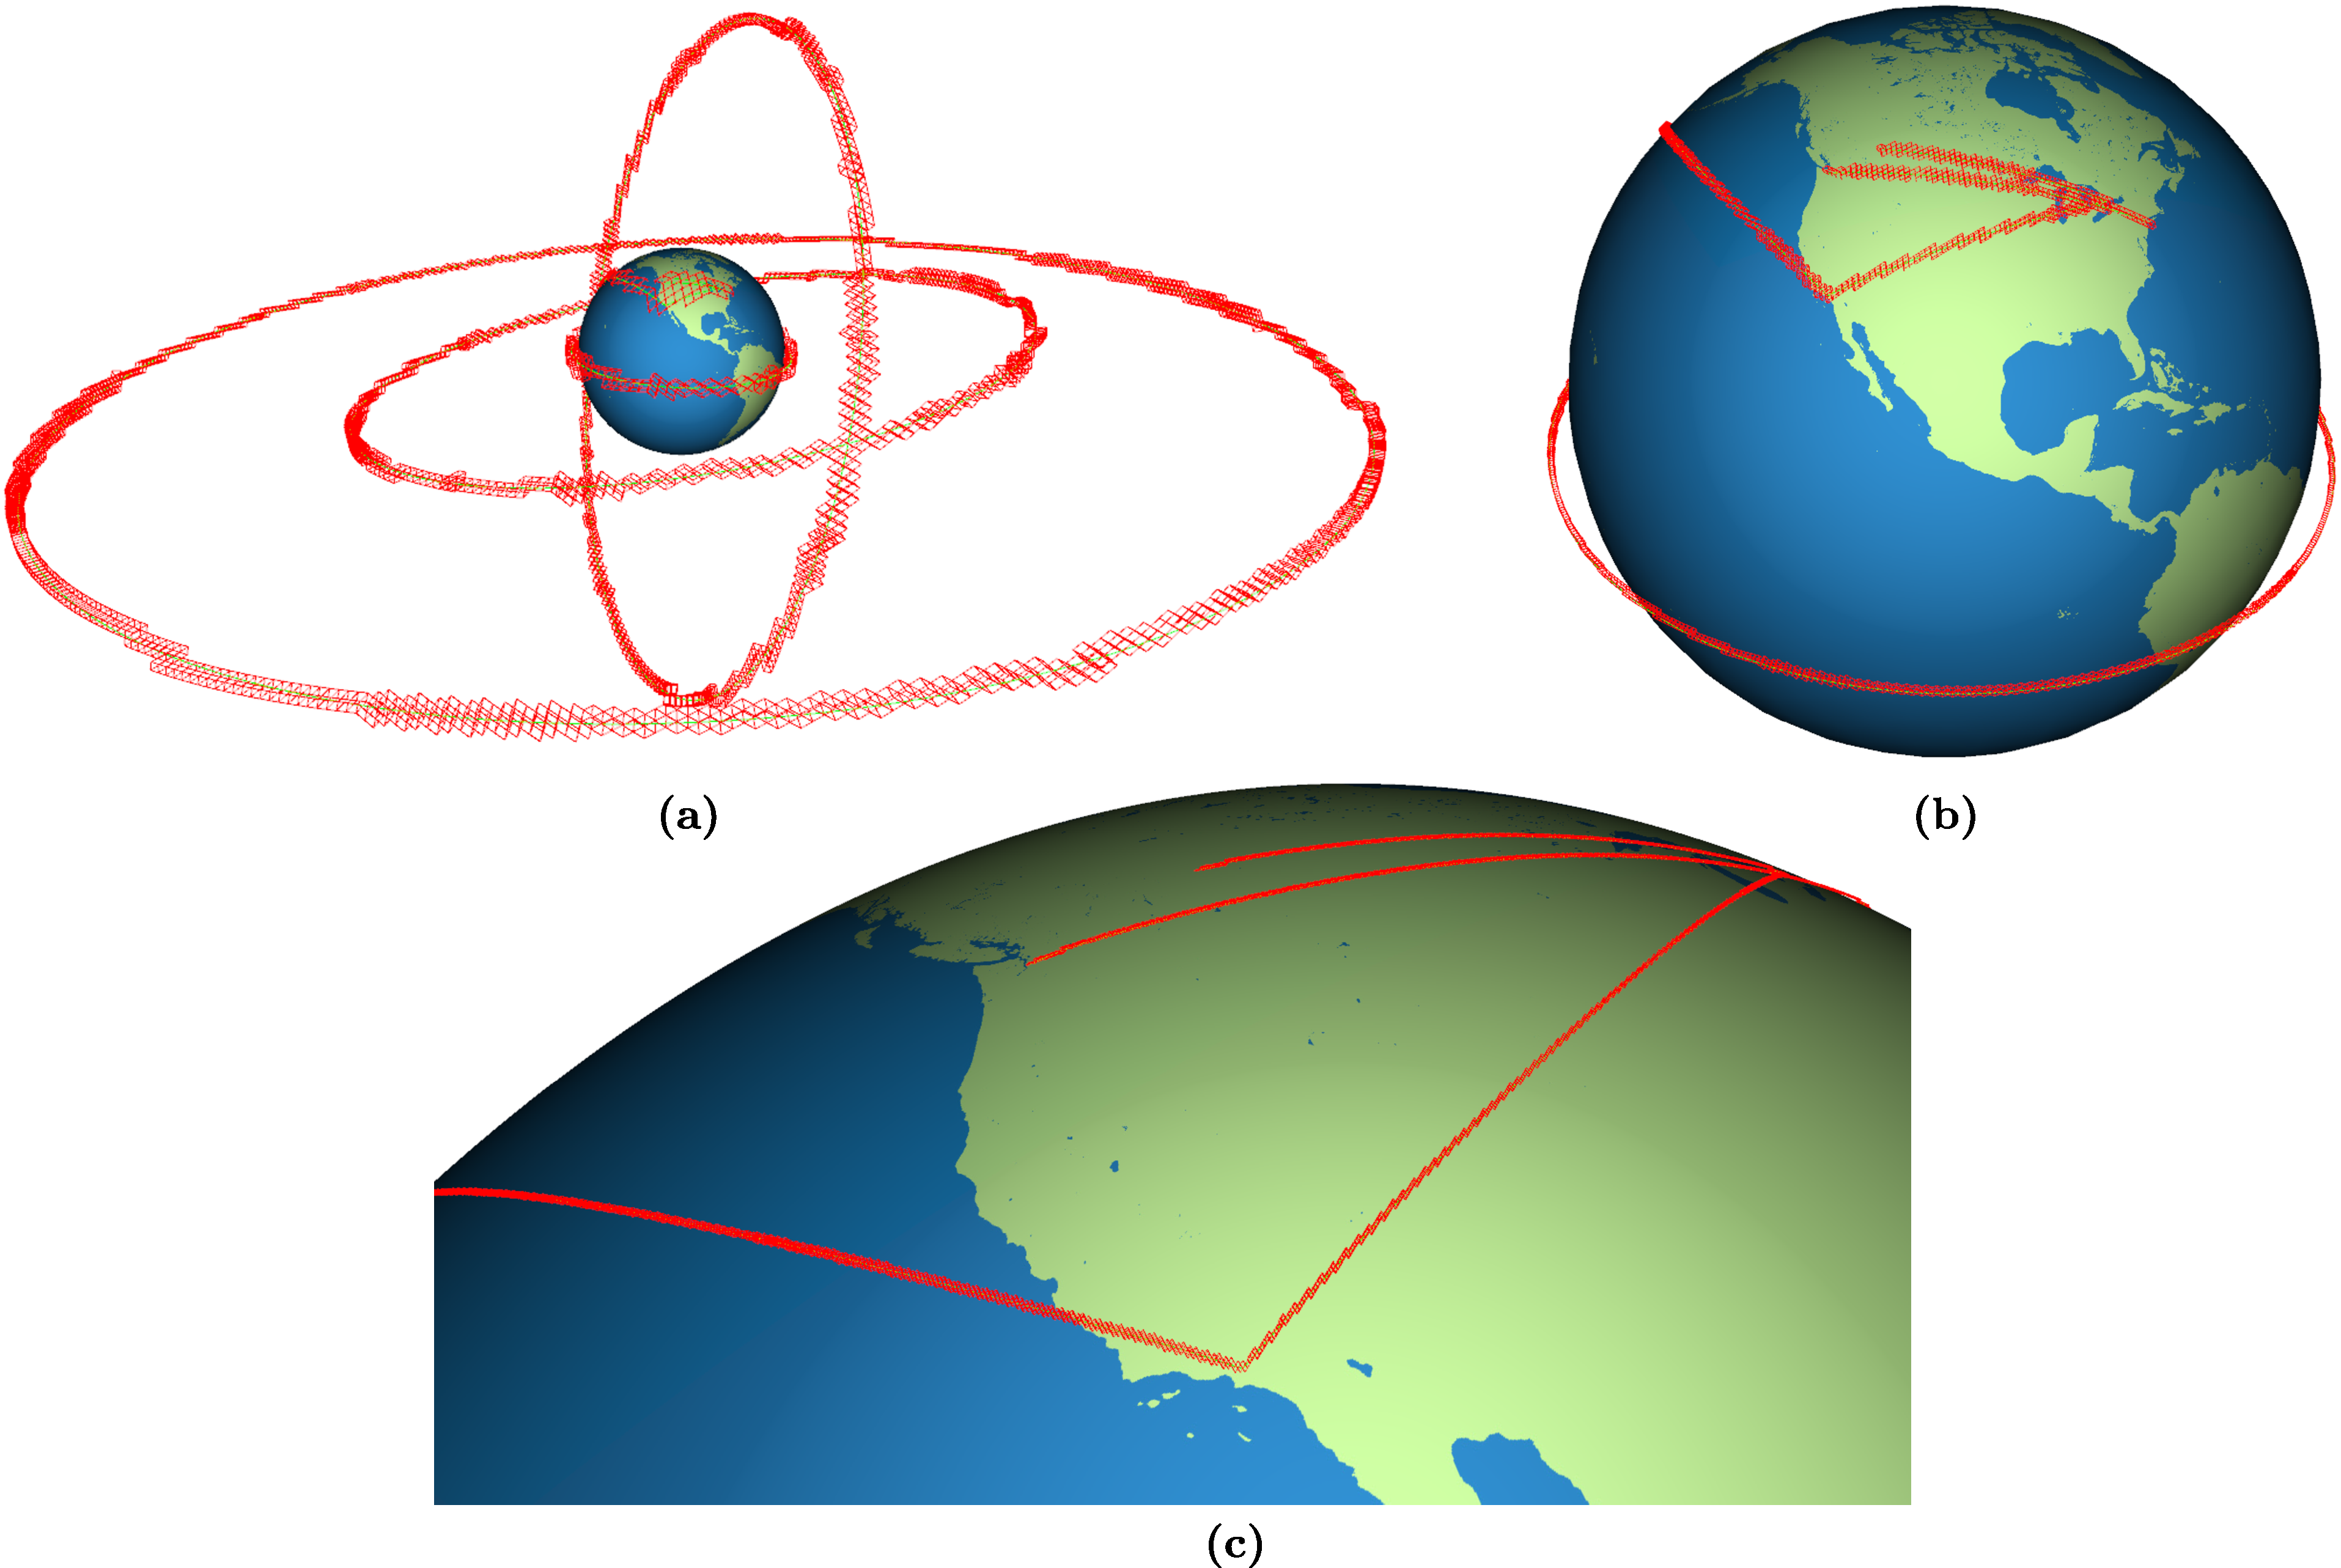
\includegraphics[width=\columnwidth]{satellites.pdf}
	\caption{Flight paths and satellite orbits rasterized in a 3D DGGS.
		All paths and orbits are rasterized at the same grid resolution of \textbf{(a)} 7, \textbf{(b)} 10, and \textbf{(c)} 13}
	\label{fig:satellites}
\end{figure}


Figure~\ref{fig:satellites} shows several generated flight paths and satellite orbits represented in a 3D DGGS at increasing resolutions.
The input DGGS for this example uses a rhombic triacontahedron as the initial polyhedron, standard 1:4 quadrilateral refinement, and a simple normalization projection.
The 3D DGGS has a target aspect ratio of one, a radial mapping exponent of one, and a radial range of 10.66$R$ (67,957~km).
These parameters were chosen to ensure that cells are as compact as possible.

\section{Urban Planning}
The second use case is a volume-preserving 3D grid for the purpose of urban planning and management.
A volume-preserving grid is useful for quickly estimating the volume of a feature that has been rasterized in the grid by multiplying the number of cells by their volume.
This use case also shows the ability of our 3D DGGS to handle small scale data in addition to the much larger scale data showcased in the previous one.


\begin{figure}[h]
	\centering
	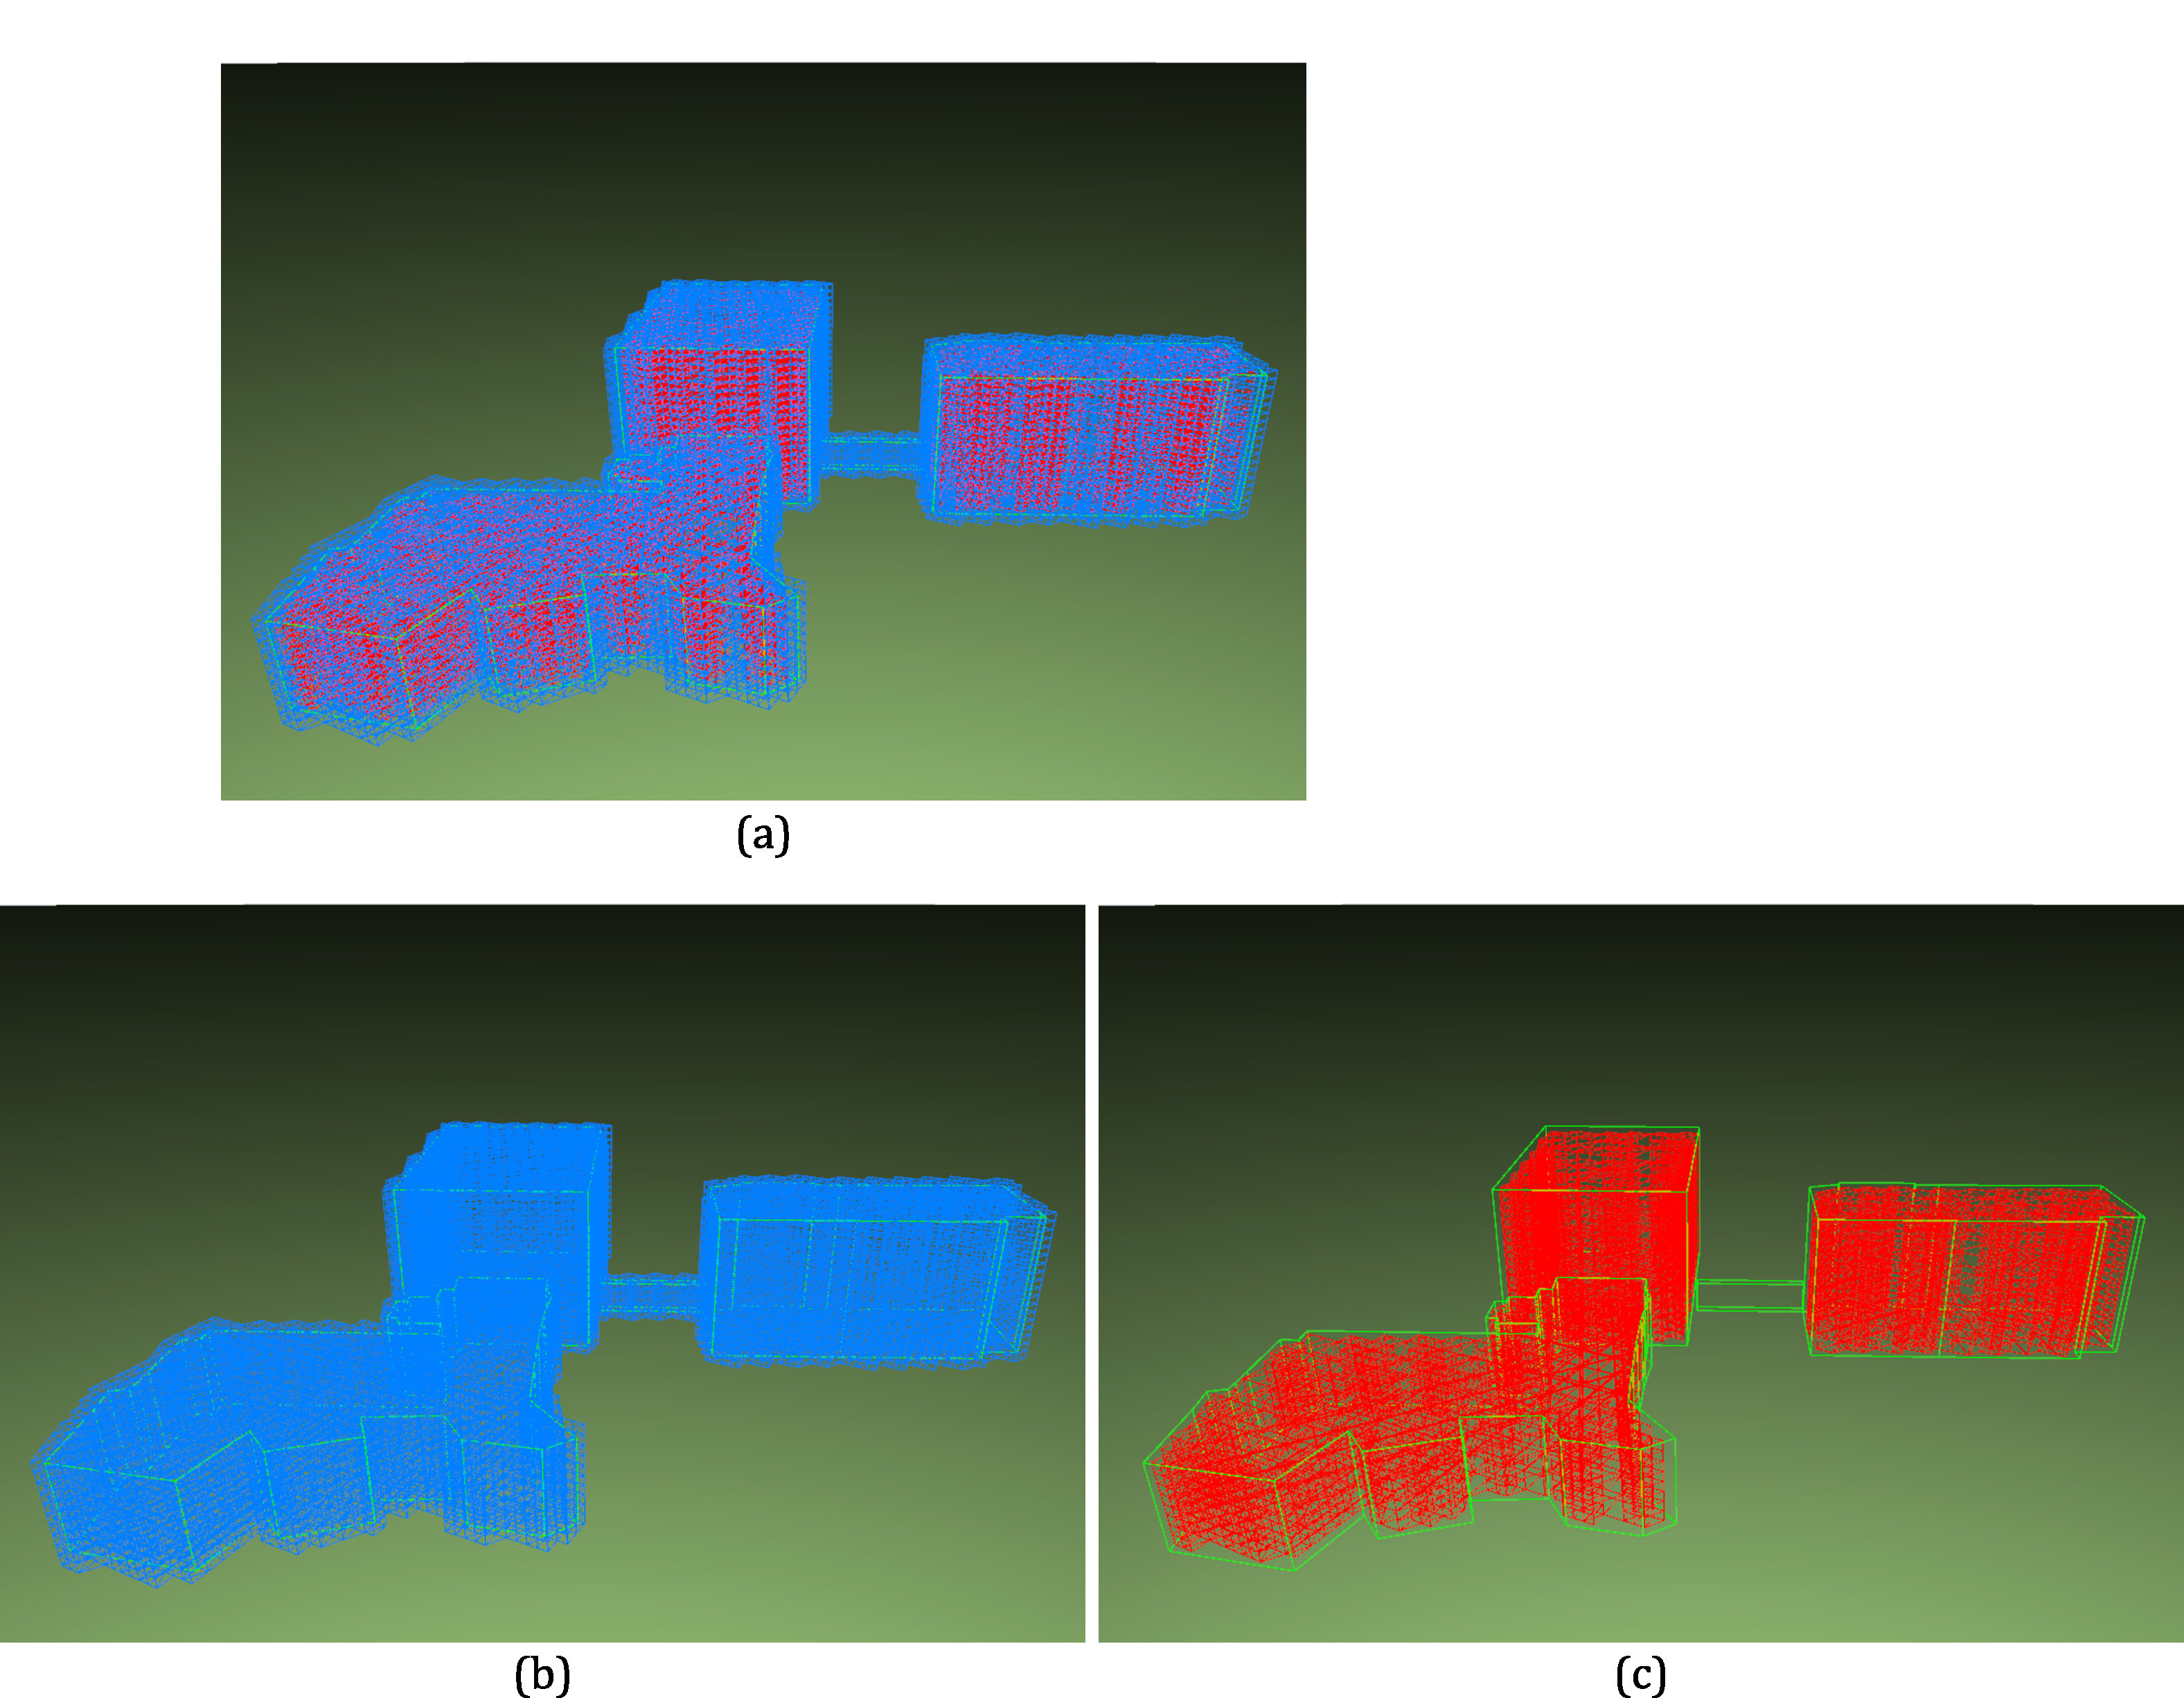
\includegraphics[width=\columnwidth]{buildings.pdf}
	\caption{A collection of buildings from the University of Calgary rasterized in a 3D DGGS at resolution 21.
		In \textbf{(a)}, both interior and boundary cells are shown, whereas \textbf{(b)} and \textbf{(c)} show only boundary and interior cells, respectively}
	\label{fig:urbanplanning}
\end{figure}


Figure~\ref{fig:urbanplanning} shows several buildings represented in a 3D DGGS, with the building geometries obtained from Open Street Map\footnote{\url{www.openstreetmap.org}}.
The input DGGS for this example uses a disdyakis triacontahedron as the initial polyhedron, a non-standard 1:4 triangle refinement to maintain the relative shape of triangles, and the vertex oriented great circle slice and dice projection~\cite{van2006slice} to preserve area~\cite{hallDT}.
The 3D DGGS has a target aspect ratio of one, a radial mapping exponent of three to achieve perfect volume preservation (excluding the central layer), and a maximum radius of 1.33$R$ (8495~km).


\section{Atmospheric Properties}
The final use case we look at is using a 3D DGGS to resample atmospheric forecasts, such as those generated by numerical weather prediction models.
These datasets typically have a much higher vertical resolution than surface resolution, due to how quickly properties such as temperature and wind speed tend to change in these two dimensions.
To accommodate this with our 3D DGGS, we can specify an appropriate aspect ratio for cells to ensure the vertical and surface resolution matches as closely as possible that of the input data.


\begin{figure}[h]
	\centering
	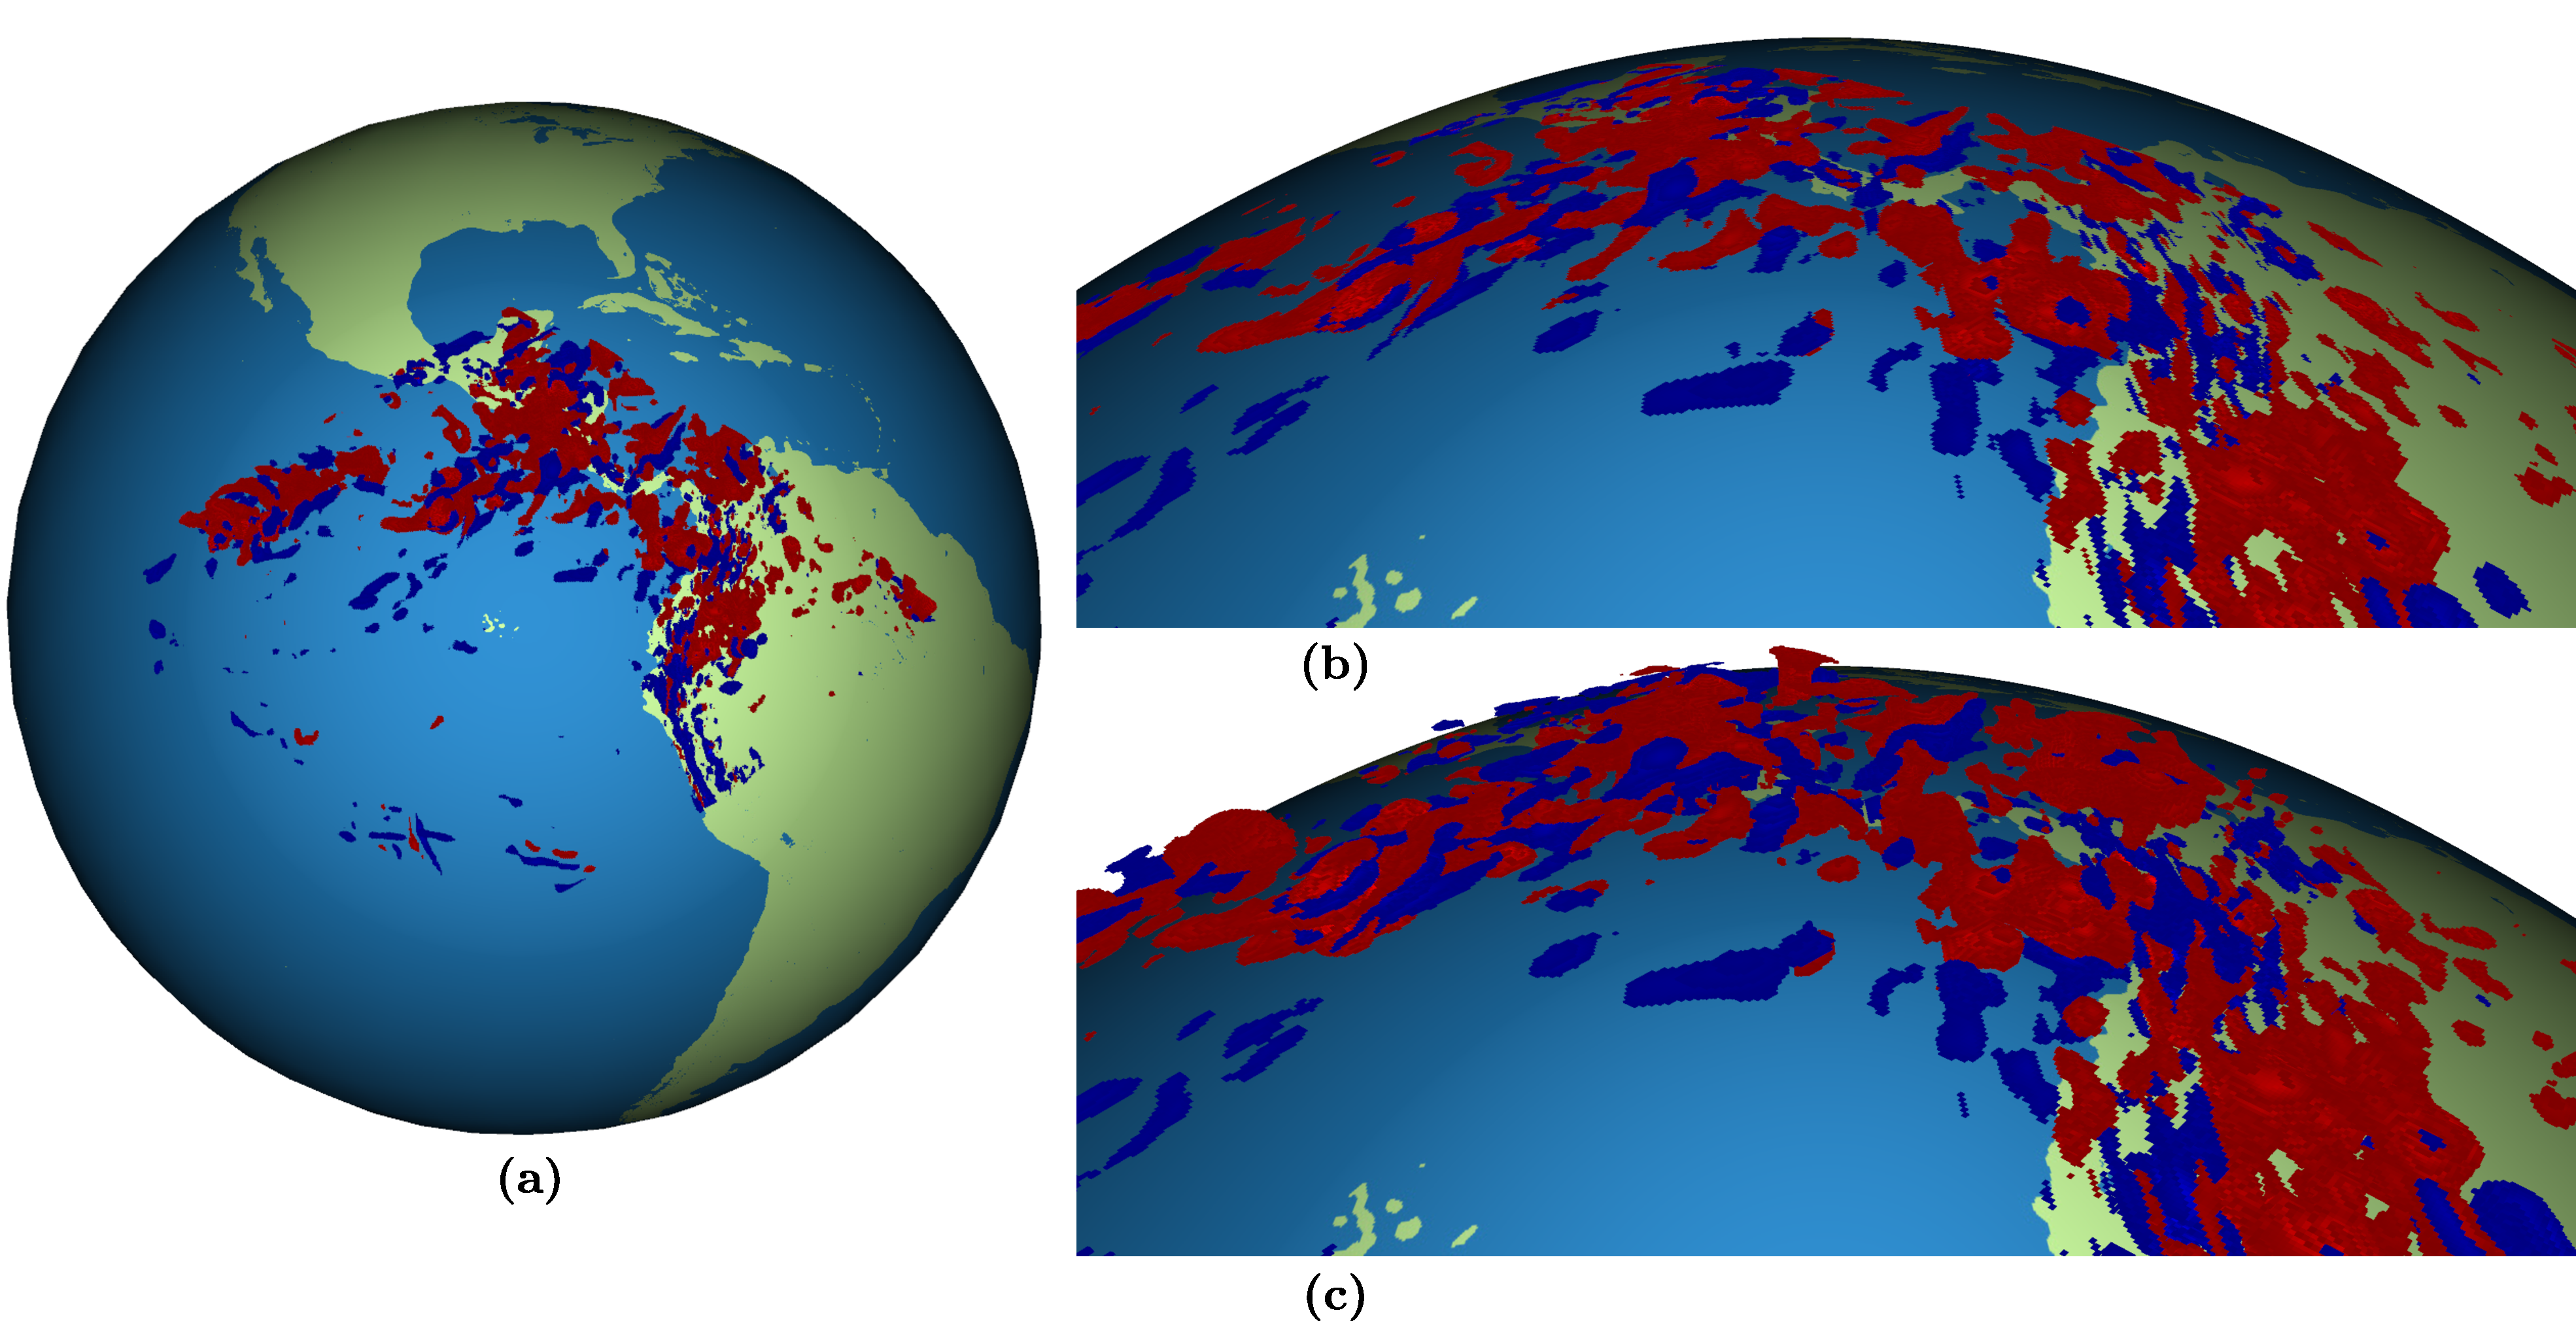
\includegraphics[width=\columnwidth]{atmosphere.pdf}
	\caption{Vertical wind speed (mbar/s) sampled into a 3D DGGS at resolution 9.
		Negative velocity, which corresponds to an upward wind, is shown in red.
		Positive velocity, which corresponds to a downward wind, is shown in blue.
		Velocities with magnitude less than 0.25 mbars/s are not shown to reduce clutter and highlight regions with the highest speeds.
		In \textbf{(a)} and \textbf{(c)}, the altitude of cells is scaled by a factor of 15 to better show changes in altitude.
		In \textbf{(b)}, altitude is shown at its true scale}
	\label{fig:atmosphere}
\end{figure}


Figure~\ref{fig:atmosphere} shows vertical wind speed from the ERA5 dataset~\cite{era5} sampled into a 3D DGGS.
The input DGGS for this example is the same as the one used for the aircraft and satellite paths.
However, this 3D DGGS has a target aspect ratio of 31.7, a radial mapping exponent of one, and a maximum radius of 1.33$R$ (8495~km).


\subsection{Discussion}
The above examples are only a small subset of the many potential applications of our 3D DGGSs.
Despite this, they show not only the useful properties achievable by the method (support for large ranges of altitudes, volume preservation between cells, custom cell aspect ratio, and support for multiple scales of data) but also demonstrate the ease at which new 3D global grids can be created.
Given a conventional DGGS that provides the required operations, creating a 3D DGGS is as simple as providing the surface grid and four clearly defined parameters for the 3D one.
Since creating a 3D DGGS that is ideal for every application is not possible, this allows quick iterations on creating and comparing different 3D grids to find the ideal one for each application.
\chapter{Discussion} \label{chap:discussion}
Nearing the end of the thesis, an important question to address is what 3D DGGS to use for which applications.
More specifically---of the grids we propose---how do they compare and in which situations should each approach be used?
This thesis explores two approaches for creating different 3D DGGS's: modifications to SDOG refinement and a 2D DGGS grid extension technique.
We present these two approaches as separate methods, with some similarities between the two shown in the radial mapping functions.
However, SDOG itself can be generated from the grid extension method, with the input DGGS being DQG.
Furthermore, our modifications to SDOG can also be generated, where the input DGGS is DQG with the corresponding latitude modifications, and the 3D DGGS uses the corresponding radial mapping.


In this chapter, we briefly discuss the benefits and drawbacks of the different 3D DGGS's we proposed in this thesis.
This discussion is meant as a general guide for the choice of 3D DGGS; specific recommendations depend too heavily on the exact details of the intended use case.
We also look at some considerations when choosing a maximum grid radius for a 3D DGGS.


\subsubsection{SDOG Modifications}
Comparing our modified SDOG grids, the volume method is a good choice if volume preservation is a high priority in the 3D DGGS.
While this method significantly sacrifices compactness, this is a necessary tradeoff to achieve volume preservation in SDOG. Additionally, when using our direct algorithms, encoding and decoding are not significantly less efficient than those for conventional SDOG.
In comparison, the balanced method can create a grid with more acceptable tradeoffs between cell volume and compactness, but the algorithms are less efficient than for the volume method.
Finally, the latitude method is unlikely to be worth using over conventional SDOG due to the marginal volume preservation gains compared to the efficiency losses in encoding and decoding.


\subsubsection{Grid Extension Method}
For the grid extension in general, several properties of the 3D DGGS are derived from---or entirely determined by---the input DGGS.
For example, area preservation in the input DGGS determines if volume preservation in the 3D one is possible, and the surface refinement factor determines the complexity of radial refinement.
Thus, choosing the correct 2D DGGS is the most critical step in creating the ideal 3D DGGS for a given application.
Regarding DQG---and thus SDOG---some of the main benefits are the efficient coding algorithms and the use of spherical coordinates for defining the grid, which means no conversions to and from Cartesian coordinates are needed.
However, degenerate connectivity on the surface (as opposed to only with changing altitude) and polar singularities make this approach less ideal in situations where uniform coverage of the entire Earth is needed.


\subsubsection{Maximum Grid Radius}
A crucial component not yet discussed in this thesis is how to chose an appropriate maximum radius for a 3D DGGS.
The most obvious consideration is to ensure this value is large enough to support the range of altitudes expected in the intended use case.
However, the maximum radius also determines which regions of the grid contain which altitude, and most importantly, where the boundaries between shells reside.
Ideally, these shell boundaries should not be near critical altitudes with large amounts of data.
Having the important altitudes on or near shell boundaries means regions directly above and below will have varying cell shape, potentially varying cell size, and degenerate connectivity; this is not ideal.
Therefore, the maximum grid radius should be chosen such that important regions are in or near the middle of shells.
If multiple altitudes are considered important, this may not always be possible to achieve for them all.
For only one altitude, though, this is easily done.

Let $R_d$ be the specific radius (in most applications, the Earth's surface) we want in the middle of a shell.
Recall that boundaries of shells (in reference space) are located at integer powers of $\alpha$ times $R_\mathrm{max}$ (refer back to \cref{fig:sdog-shells,fig:prismatoid-shells}).
Therefore, the middle of shell zero is located at
%
\begin{equation*}
\left( \alpha + \frac{1}{2} (1 -\alpha) \right) R_\mathrm{max} = \frac{ \alpha + 1 }{2} R_\mathrm{max},
\end{equation*}
%
and multiplying this by $a^s$ gives the middle of shell $s$.
From this we obtain
%
\begin{equation*}
R_d = \frac{ \alpha^s \left( \alpha + 1 \right) }{2} R_\mathrm{max}
\end{equation*}
%
which we solve for $R_\mathrm{max}$ to get
%
\begin{equation*}
R_\mathrm{max} = \frac{2 R_d}{ \alpha^s \left( \alpha + 1 \right) }.
\end{equation*}
%
Then, we simply solve for smallest $s$ that results in value greater than or equal to maximum radius needed to support.

\chapter{Conclusion} \label{chap:conclusion}
With the amounts of 3D geospatial data becoming available, techniques for integrating and managing such data are becoming increasingly important.
A recent approach for aiding in this is the 3D DGGS.
A 3D DGGS provides an indexed multiresolution hierarchy of cells where geospatial data is associated with cells that correspond to the appropriate regions of the Earth.
The two main classes of 3D DGGS are embedded and Earth-centric, with the latter typically preferred as they provide a more natural representation of the planet.
However, a common challenge with Earth-centric 3D DGGS's is the reduction in cell compactness and volume approaching the singularity at the centre of the Earth.
One potential solution to this problem is semiregular degenerate refinement.


This thesis explored the application of semiregular degenerate refinement techniques for the purpose of creating Earth-centric 3D DGGS's.
First, we showed how modifying the location of splitting surfaces can improve volume preservation, specifically looking at the case of SDOG.
Building on this, we derived a general method for extending an arbitrary 2D DGGS to the third dimension.
To define coding operations for these two approaches, we first derived a set of radial and latitude mapping functions.
These mappings allowed us to define coding algorithms that operate in a more uniform grid space while still having volume preservation in reference space.
For SDOG, we also presented direct coding algorithms that run in constant time in comparison to the linear time of their hierarchical counterparts.
Additionally, we presented neighbour, child, and parent operations for SDOG and the grid extension method in general.
The grid extension method has been fully implemented and used to demonstrate three potential use cases of 3D DGGS using three different grid systems.
Given an input DGGS, creating the 3D DGGS is instant and only requires three parameters clearly defined and explored in this thesis.


Looking back at \cref{chap:introduction}, our goals were for our 3D DGGS's to support unbounded ranges of altitude, equal (or near-equal) volume cells, efficient operations, and interoperability with 2D DGGS's.
Support for unbounded ranges of altitudes is achieved as a direct result of using semiregular degenerate refinement, and is also clearly demonstrated in \cref{chap:8:sats}.
We achieve equal volume cells (excluding degenerate cells) for SDOG in the volume method.
Furthermore, volume preservation is also possible for the grid extension method if the input DGGS is area-preserving by using the appropriate radial mapping function.
Finally, the algorithms provided in \cref{chap:coding} are efficient, and the use of surface indices from the input DGGS ensures consistency and interoperability between the 2D and 3D systems.


\section{Limitations and Future Work}
The field of 3D DGGS is relatively young and unexplored, especially compared to the rich body of research for their 2D counterparts.
While this thesis provides important contributions to this developing field, there are still many significant future works to be done.
Despite the generality of our grid extension method, it can only create one particular type of 3D DGGS.
While we believe this type of 3D DGGS is useful in many applications, it is certainly not the ideal type for all.
The method also has its limitations.


First, we do not provide a general method for linearizing the layer parameterization ($s$, $j$, and $k$) or for combining this with the surface index of the input DGGS.
Indices with good locality properties are essential for a DGGS, as this helps minimize the number of cache misses and disk seeks when retrieving data.
General methods for linearizing indices that represent different dimensions (i.e. surface vs. radial) could also be extended to the time dimension for a 4D DGGS.


Second, we only explore our grid extension method in the context of a sphere-based input DGGS.
However, the Earth is more accurately approximated with an oblate spheroid, and correspondingly, there exist ellipsoid-based DGGS's.
While we believe our method would also work for ellipsoid based DGGS's, more careful exploration is needed to justify this claim.


Finally, geospatial data represented as polylines, polygons, point clouds, 3D meshes, and other complex geometry require their own encoding algorithms beyond those for points.
We implemented encoding algorithms for polylines and polygonal prisms in \cref{chap:usecases}; however, they were only meant to serve as a proof of concept.
General and efficient versions of these algorithms are vital for creating a more robust 3D DGGS.


Another challenge with volumetric Digital Earth applications, in general, is that of occlusion in visualizations.
Data at higher altitudes blocks the view of lower altitudes.
This issue is especially present when trying to visualize subterranean data while maintaining a view of the planet's surface for reference.
The structure of a 3D DGGS may be able to aid in such occlusion issues by allowing slices and layers of cells to be viewed independently of other cells in the grid.

% end

\appendix

\bibliographystyle{ieeetr}
%\nocite{*}
\bibliography{sources}

\chapter{Copyright Permissions}
This appendix contains the copyright permission for the reuse of \cref{fig:edge-continuity} from~\cite{hennerdal2015beyond}.
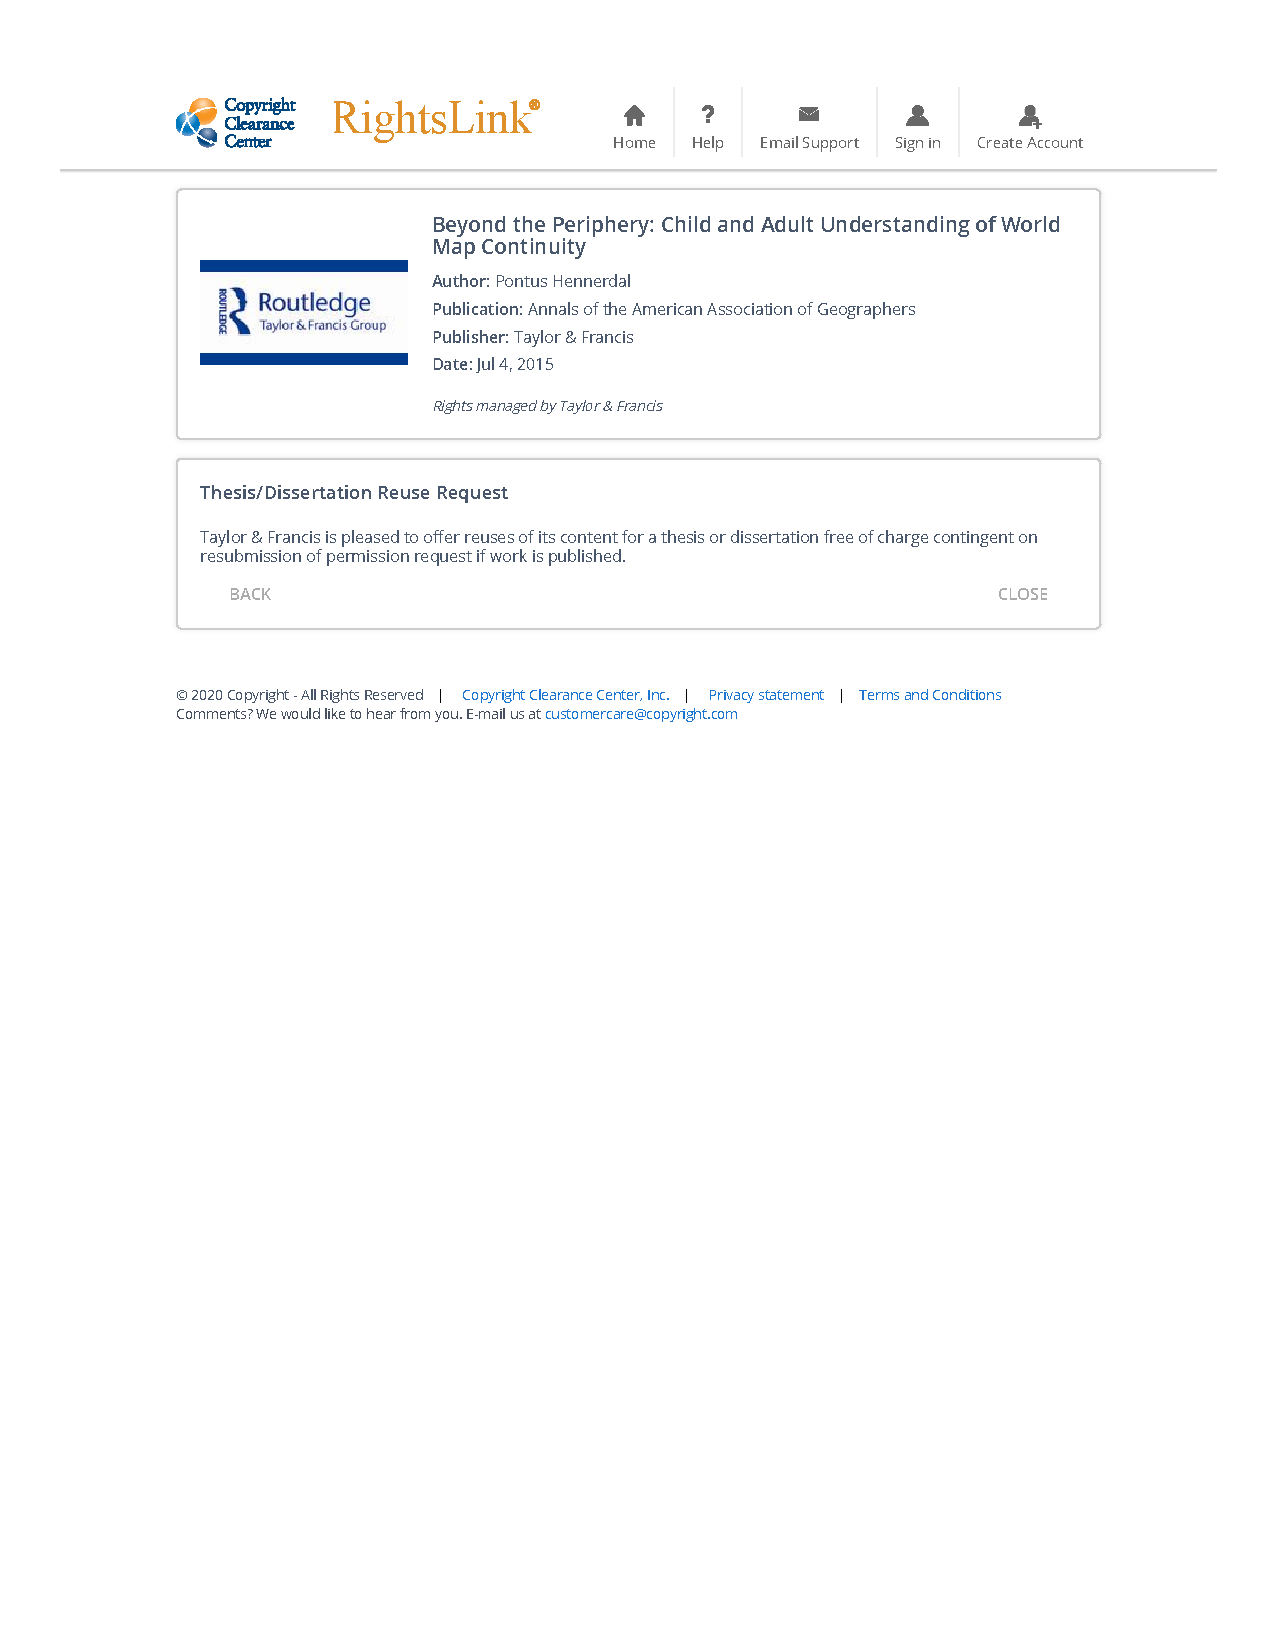
\includepdf[pages=-,pagecommand={},width=\paperwidth]{copyright.pdf}

\end{document}
